%%%%%%%%% espcrc1.tex %%%%%%%%%%
%
% $Id: espcrc1.tex 1.2 2000/07/24 09:12:51 spepping Exp spepping $
%
\documentclass[a4paper,12pt]{report}
\usepackage{footnote}
\usepackage{graphics}
\usepackage{sidecap}
\usepackage{layouts}
\usepackage{epsf}
\usepackage{epsfig}
\input epsf
\usepackage{times}
\usepackage[T1]{fontenc}
\usepackage[latin1]{inputenc}
\usepackage{geometry}
%\geometry{verbose,tmargin=0.7in,bmargin=0.5in,lmargin=0.4in,rmargin=0.4in}
%\setcounter{secnumdepth}{3}
%\setcounter{tocdepth}{3}
\geometry{verbose,a4paper,tmargin=1in,bmargin=1in,lmargin=1.in,rmargin=0.7in}
\usepackage{graphicx,psfrag}
\usepackage{setspace}
\usepackage{epsf}
\usepackage{amsmath}
\usepackage{amssymb}
\usepackage{bm}
%\doublespacing
\usepackage{rotating}
\raggedbottom
\textwidth  6.0 in
\textheight 8.5 in
%\oddsidemargin 0.15in
%\makeatletter
\newcommand{\plus}{\raisebox{.3\height}{\scalebox{.6}{+}}}
\newcommand{\minus}{\raisebox{0\height}{\scalebox{1}{-}}}
\begin{document}
%\pagestyle{empty}
\begin{flushright}
\vspace{-1cm}
\centerline{New Research Proposal to Jefferson Lab PAC 44}
\def\beqn{\begin{eqnarray}}
\def\eeqn{\end{eqnarray}}

\def\Journal#1#2#3#4{{#1} {\bf #2} (#4) #3 }
\def\PPNP{{ Prog. Part. Nucl. Phys.}}
\def\NIMA{{ Nucl. Instrum. Meth.} A}
\def\NIMB{{ Nucl. Instrum. Meth.} B}
\def\NCA{{ Nuovo Cimento} A}
\def\PHYS{{ Physica}}
\def\NPA{{ Nucl. Phys.} A}
\def\MATH{{ J. Math. Phys.}}
\def\PRO{{ Prog. Theor. Phys.}}
\def\NPB{{ Nucl. Phys.} B}
\def\PLA{{ Phys. Lett.} A}
\def\PLB{{ Phys. Lett.} B}
\def\PLD{{ Phys. Lett.} D}
\def\PL{{ Phys. Lett.}}
\def\PRL{ Phys. Rev. Lett.}
\def\PREV{ Phys. Rev.}
\def\PREP{ Phys. Rep.}
\def\PRA{{ Phys. Rev.} A}
\def\PRD{{ Phys. Rev.} D}
\def\PRC{{ Phys. Rev.} C}
\def\PRB{{ Phys. Rev.} B}
\def\ZPC{{ Z. Phys.} C}
\def\ZPA{{ Z. Phys.} A}
\def\ANNP{ Ann. Phys. (N.Y.)}
\def\RMP{{ Rev. Mod. Phys.}}
\def\CHEM{{ J. Chem. Phys.}}
\def\INT{{ Int. J. Mod. Phys.} E}
\def\INTA{{ Int. J. Mod. Phys.} A}
\def\EPJC{{ Eur. Phys. J.} C}
\def\JHEP{{ JHEP}}
\def\SJNP{{ Sov. J. Nucl. Phys.}}
%
\newcommand{\la}{\langle}
\newcommand{\ra}{\rangle}
\newcommand{\zh}{z}
\newcommand{\xbj}{x_{\scriptscriptstyle B}}
%
\newcommand{\Epgb}{$\vec ep~\rightarrow~ep(p,\Delta, N^*)\gamma~$}
\newcommand{\Epgl}{$\vec e\vec p~\rightarrow~ep(p,\Delta, N^*)\gamma~$}
\newcommand{\Eppiz}{$ep~\rightarrow~ep\pi^0~$}
\newcommand{\Enpip}{$ep~\rightarrow~en\pi^+~$}
\newcommand{\EppiD}{$ep~\rightarrow~e\pi \Delta~$}
\newcommand{\Epeta}{$ep~\rightarrow~ep\eta~$}
\newcommand{\Epr}{$ep~\rightarrow~ep\rho~$}
\newcommand{\EpX}{$ep\rightarrow epX~$}
\newcommand{\EpKY}{$ep~\rightarrow~eKY~$}
\newcommand{\vEpg}{$\vec ep~\rightarrow~ep\gamma~$}
\newcommand{\xidef}{$\xi=x_B\frac{1+\frac{Delta^2}{2Q^2}}{2-x_B+x_B\frac{Delta^2}{2Q^2}}$}
\def\gevc2{(GeV/c)$^2$}
\newcommand{\EpgX}{$ep~\rightarrow~ep\gamma X~$}
%%%%%%%%%%%%%%%%%%%%%%%%%%%%%%%%%%%%%%%%%%%%%%%%%%%

\renewcommand{\topfraction}{0.95}
\renewcommand{\bottomfraction}{0.95}
\renewcommand{\textfraction}{0.05}
\renewcommand{\floatpagefraction}{0.95}
\end{flushright}

\bigskip
%\vskip 0.5cm
{\Large{\centerline {\bf Proposal of extension of the CLAS12 run-group Cb (ND$_3$ target)}}}
%{\Large{\centerline {\bf CLAS12 and a longitudinally polarized deuterium target}}}

\vskip 0.5cm

\centerline{S. Niccolai\footnote{co-spokesperson}$^,$\footnote{contact person, email: silvia@jlab.org}, G. Charles, R. Dupr\'e, M. Guidal,}
\centerline{D. Marchand, C. Munoz Camacho, E. Voutier}
\centerline{\it Institut de Physique Nucl\'eaire d'Orsay, 91406 Orsay, France}
\vskip 0.4cm
\centerline{A. Biselli\footnotemark[1]}
\centerline{\it Fairfield University, Fairfield Connecticut 06824}
\vskip 0.4cm
\centerline{C. Keith\footnotemark[1], H. Avakian, V. Burkert, A. Deur, F.X. Girod, L. Elouadrhiri,} 
\centerline{V. Kubarovsky, K. Park, P. Rossi, S. Stepanyan, M. Ungaro}
\centerline{\it Thomas Jefferson National Laboratory, Newport News, VA 23606}
\vskip 0.4cm
\centerline{S. Pisano\footnotemark[1], V. Lucherini, M. Mirazita}
\centerline{\it INFN, Laboratori Nazionali di Frascati, 00044 Frascati, Italy}
\vskip 0.4cm
\centerline{D. Sokhan\footnotemark[1], D. Ireland, D. McGregor, B. McKinnon, G. Murdoch, B. Seitz}
\centerline{\it University of Glasgow, Glasgow, Scotland}
\vskip 0.4cm
\centerline{S. Kuhn\footnotemark[1]}
\centerline{\it Old Dominion University, Norfolk, VA 23529}
\vskip 0.4cm
\centerline{M. Battaglieri, A. Celentano, R. De Vita, E. Fanchini, M. Osipenko, M. Ripani, M. Taiuti}
\centerline{\it Istituto Nazionale di Fisica Nucleare, Sezione di Genova and }
\centerline{\it Dipartimento di Fisica, Universit\`a di Genova, Genova, Italy 16146}
\vskip 0.4cm
\centerline{D. Crabb, D. Day, D. Keller}
\centerline{\it University of Virginia, Charlottesville, VA 22904}
\vskip 0.4cm
\centerline{I. Balossino, L. Barion, G. Ciullo, M. Contalbrigo, P. Lenisa,}
\centerline{A. Movsysian, L. Pappalardo, M. Turisini}
\centerline{\it INFN, Istituto Nazionale di Fisica Nucleare, Sezione di Ferrara, Ferrara, Italy 44122}
\vskip 0.4cm
\centerline{A. D'Angelo, L. Lanza, A. Rizzo, I. Zonta}
\centerline{\it Universit\`a di Roma Tor Vergata and INFN Roma Tor Vergata, Roma, Italy 00133}
\vskip 0.4cm
\centerline{V. Bellini, F. Mammoliti, G. Russo, C.M. Sutera}
\centerline{\it Istituto Nazionale di Fisica Nucleare, Sezione di Catania, Catania, Italy 95123} 
\vskip 0.4cm
\centerline{J. Ball, M. Defurne, M. Gar\c{c}on, H. Moutarde, S. Procureur, F. Sabati\'e}
\centerline{\it CEA, Centre de Saclay, Irfu/Service de Physique Nucl\'eaire, 91191 Gif-sur-Yvette, France}
\vskip 0.4cm
\centerline{W.R. Armstrong, K. Hafidi, M. Hattawy}
\centerline{\it Argonne National Laboratory, Argonne, IL 60439}
\vskip 0.4cm
\centerline{P. Bosted, K. Griffioen}
\centerline{\it College of William and Mary, Williamsburg, VA 23187}
\vskip 0.4cm
\centerline{K. Slifer, E. Long, T. Badman, L. Hammed, M. Holtrop,}
\centerline{S. Li, D. Ruth, S. Santiesteban, R. Zielinski}
\centerline{\it University of New Hampshire, Durham, NH 03824}
\vskip 0.4cm
\centerline{T. Forest}
\centerline{\it Idaho State University, Pocatello, ID 83209}
\vskip 0.4cm
\centerline{K. Adhikari, L. El Fassi}
\centerline{\it Mississippi State University, Mississippi State, MS 39762 }
\vskip 0.4cm
\centerline{I. Skorodumina}
\centerline{\it University of South Carolina, Columbia, SC 29208}
\vskip 0.4cm
\centerline{G. Fetodov}
\centerline{\it Skobeltsyn Institute of Nuclear Physics, Lomonosov Moscow State, Russia}
\vskip 0.4cm
{\large{\centerline{\bf A CLAS Collaboration proposal}}}
\date{}

\abstract{The multi-dimensional mapping of the structure of the nucleon in terms of its partonic degrees of freedom is nowadays one of the main challenges of hadronic physics, and is at the core of the CLAS12 experimental program. Precise measurements of polarized parton distribution functions (PDFs) via deep inelastic scattering (DIS) give information on the spin content of the nucleon; the extraction of transverse momentum dependent distributions (TMDs) from semi-inclusive DIS (SIDIS) data provides the correlation between the transverse momentum and spin of the quarks; the generalized parton distributions (GPDs), accessible in exclusive electroproduction channels, finally, encode the interplay between the longitudinal momentum, the transverse position, and the spin of the quarks in the nucleon. An extensive experimental program geared towards the extraction of all the cited distributions is already scheduled for CLAS12, mainly on a proton target. In particular, 120 days on a polarized NH$_3$ target are approved. However, in order to perform the flavor separation of PDFs, TMDs, and GPDs, measurements on a neutron target, with comparable statistical precision, are necessary as well. This proposal aims at extending the running time of the approved run-group Cb, which currently provides 50 days of an 11-GeV electron beam impinging on a longitudinally polarized deuterium target (plus $\sim10$ days for target overhead and beam-polarization measurements), to 110 days of total duration (plus 23 days of overhead). For 50 days of the extension the same experimental setup of RG Cb will be used, with a beam current of 10 nA, while the Forward Tagger will be included for 10 days of low-luminosity running, at 5 nA. Assuming that run-group Cb includes a total of 60 days between production and ancillary runs, this proposal requests 73 new PAC days. The driving motivations for this extension are the measurements of single and double target-spin asymmetries for deeply virtual Compton scattering on longitudinally polarized neutrons (nDVCS), of double and single spin asymmetries for SIDIS (with both pions and kaons), and double spin asymmetries for DIS on the deuteron. Considering the lower polarization of the neutron on ND3 (40\%) with respect to the one of the proton in NH3 (80\%) and the smaller cross sections on neutrons than on protons, the overall neutron figure-of-merit is at least a factor of 4 smaller than for the proton. At a minimum, matching the integrated luminosity on protons with that on neutrons is necessary to perform the flavor separation of the aforementioned parton distributions, binned in the relevant kinematic variables. 
These data will also allow pioneering first-time measurements, such as polarized timelike Compton scattering, deeply-virtual meson electroproduction, and semi-inclusive di-hadron production off a longitudinally polarized neutron.}
\newpage
\tableofcontents{}
%\newpage
%\listoftables{} 
%\listoffigures{}
%\newpage
%\setcounter{page}{1}

\chapter{Run-group extension summary}
\section{Motivation for the run-group extension request}
This proposal is being submitted in response to the specific requests made by PAC43 in the report motivating the conditional approval of Experiment C12-15-004. 
Here we request the extension to 110 days, plus overhead, of the existing CLAS12 run-group Cb, which currently has 50 approved days of running of 11 GeV electron beam on a longitudinally polarized ND$_3$ target. 
The physics topics that will be studied thanks to this extensions cover two categories of the experimental program for the 12-GeV upgrade of Jefferson Lab: 
\begin{itemize}
\item{``The longitudinal structure of the hadrons (Unpolarized and polarized parton distribution functions - PDFs)'', with the measurement of deep inelastic scattering on longitudinally polarized deuterium (this proposal extends the already approved CLAS12 experiments E12-06-109 and E12-09-007b);}
\item{``The 3D structure of the hadrons (Generalized Parton Distributions - GPDs - and Transverse Momentum Distributions - TMDs)'', with the measurement of deeply virtual Compton scattering (DVCS) and semi-inclusive deep inelastic scattering (SIDIS) on longitudinally polarized neutron (for the SIDIS case, this proposal extends the already approved CLAS12 experiments E12-07-107 and E12-09-009).}
\end{itemize}
For both of these two categories, which are the main focus of the experimental program of CLAS12, the issue of quark-flavor separation of the three kinds of parton distributions extracted from the data (PDFs, GPDs, and TMDs) is fundamental. From the experimental point of view, flavor separation requires to take data to measure DIS, SIDIS and DVCS on both hydrogen and deuterium targets. Ideally, the statistical weight of proton and neutron data should be equal. The currently approved experimental program of CLAS12 foresees, on the one hand, an almost equal number of allocated days for unpolarized proton and deuterium targets (100 for the former, 80 for the latter). On the other hand, in the case of longitudinally polarized targets hydrogen has an allocated beam time (120 days) which is more than twice the one currently approved for deuterium (50 days). This discrepancy becomes even bigger considering that the polarization of the neutrons in ND$_3$ ($\sim 40$\%) is half of that of protons in NH$_3$ ($\sim 80$\%), and that the cross sections on the neutron are typically about half of those on the proton. Doubling the currently approved run-time on ND$_3$ will bring the deuteron statistics closer to that of the proton. 

In the case of DIS, increasing the statistics on polarized deuteron by a factor of two will reduce the uncertainty on polarized parton distributions for $d$ quarks, in the large-$x$ region, as well as for gluons and the strange quark sea at moderate-to-large $x$. This will be important to understand nuclear effects on the extraction of $\Delta d$ at high $x$, and to map out the asymptotic behavior of all quark distributions provided by Jefferson Lab's 12-GeV beam. 

In the case of SIDIS, the benefits of an increased statistics on ND$_3$ will be mostly evident in the high-$p_T$ region, where the existing TMD-based models are less constrained and their predictions for the SIDIS single and double target-spin asymmetries differ the most. Such benefits will be particularly important for the kaon channels, for which the statistics are considerably smaller than for pions. Moreover, the use of the Forward Tagger, for a subset of the running time, will impact very favorably the $\pi^0$ channel, increasing the coverage in the forward region. 

As far as DVCS is concerned, the neutron sector is basically unexplored, so far. An experiment to measure beam-spin asymmetries for neutron-DVCS with an unpolarized deuterium target is currently approved for CLAS12 (and labeled ``high impact'' by the PAC), but no measurements of single and double target-spin asymmetries exist nor are planned, as of today, for longitudinally polarized deuterium target. Combining DVCS observables measured at the same kinematic points allows to extract, in a model-independent way, the Compton Form Factors (CFFs), which are linked to the GPDs. 80 days are currently approved for unpolarized deuteron. In the polarized-target case, the maximum neutron luminosity achievable with CLAS12 is about an order of magnitude (3/20) smaller than for the unpolarized-target case, and the neutron polarization is $\sim 40$\%, but, on the plus side, the expected size of the target-spin asymmetry (TSA) for nDVCS is, on average, about a factor of 5 bigger than the beam-spin asymmetry (BSA): this means that matching the running time of unpolarized and polarized deuterium will lead to relative errors for the BSA and the TSA not too far off from each other (roughly a factor of 2 bigger relative errors for the TSA than for the BSA), and improve the coverage and precision on the extracted neutron CFFs. The utilization of the Forward Tagger in 10 of the 60 days of the extension, moreover, would permit to complete the $\phi$ coverage of the asymmetries, and thus the statistical precision on the extracted CFFs, especially for the low-$t$ kinematics, which are the most crucial for Ji's sum rule. The latter relates the total angular momentum of the quarks to the second moment in $x$ of the sum of two of the GPDs ($E$ and $H$), at $t=0$.

\section{Running conditions and beam-time request}
This extension request aims to reach a total of 110 days of production running on ND$_3$, plus 23 days of ``overhead'', which includes polarized-target maintenance, runs on carbon target for background studies, M\o ller runs to measure the beam polarization, and a few days of work to install the Forward Tagger. 

The beam current will be of 10 nA, corresponding to a total luminosity on ND$_3$ of $10^{35}$ cm$^{-2}$s$^{-1}$ and to a luminosity per neutron of $1.4 \cdot 10^{34}$ cm$^{-2}$s$^{-1}$, for 100 out of 110 days, and 5 nA for the remainder 10 days. 

The experimental setup for the already approved 50 days and for 50 more days that we request will remain unchanged (it includes the standard CLAS12 and the ND$_3$ longitudinally polarized target). For 10 of the 60 extra days of production running requested in this proposal, the inclusion of the Forward Tagger will allow to detect low-angle photons and thus increase the acceptance and precision at low $t$ for nDVCS observables, and also increase the coverage for the study of the $\pi^0$ channel in SIDIS. 

The beam-time request for the extended run-group Cb is detailed in Table~\ref{beam_time_summary}, in PAC days. 

\begin{table}
\begin{center}
\begin{tabular}{|c||c|}
%\hline
%Testing and commissioning & 2 days\\
\hline
Production data taking at $10^{35}$ cm$^{-2}$s$^{-1}$ on ND$_3$ & 100 days (50 of which are already approved)\\
\hline
Production data taking at $0.5\cdot 10^{35}$ cm$^{-2}$s$^{-1}$ on ND$_3$ & 10 days (with FT)\\
\hline
Target work & 8 days\\
\hline
Production data taking on $^{12}$C target & 10 days\\
\hline 
M\o ller polarimeter runs & 2 days\\
\hline
Configuration change & 3 days \\
\hline
\hline
Total beam time request & 133 days\\
\hline
\end{tabular}
\caption{Beam-time request for the extended of Run-group Cb, in PAC days, including the already approved 50 days on ND$_3$ and 23 days of overhead and calibration runs, which are shared between the approved RG and its extension.}
\label{beam_time_summary}
\end{center}
\end{table}

Assuming 60 PAC days in total, between production and ancillary runs, for the already approved part of run-group Cb \footnote{The number of days for production and ancillary runs varies for the various proposal constituing the presently approved run group Cb. 60 days is our own estimate, including 50 days of production running, 5 days of carbon data, 4 days of target work and 1 day of M\o ller runs.}, this extension proposal requests 73 PAC days of new beam time. 

\newpage
\chapter{Deeply Virtual Compton Scattering on the neutron with a longitudinally polarized deuteron target}
\centerline{Proposal presented following the conditional approval}
\centerline{of Experiment C12-15-004 by PAC 43}
\vskip 0.4cm
\centerline{S. Niccolai\footnote{contact person, email: silvia@jlab.org}}
\centerline{\it Institut de Physique Nucl\'eaire d'Orsay, 91406 Orsay, France}
%\vskip 0.4cm
%\centerline{A. Biselli\footnotemark[1]}
%\centerline{\it Fairfield University, Fairfield Connecticut 06824}
%\vskip 0.4cm
%\centerline{C. Keith\footnotemark[1]}
%\centerline{\it Thomas Jefferson National Laboratory, Newport News, VA 23606}
%\vskip 0.4cm
%\centerline{S. Pisano\footnotemark[1]}
%\centerline{\it INFN, Laboratori Nazionali di Frascati, 00044 Frascati, Italy}
%\vskip 0.4cm
%\centerline{D. Sokhan\footnotemark[1]}
%\centerline{\it University of Glasgow}
%\vskip 0.4cm

\abstract{Measurements of Deeply Virtual Compton Scattering on the neutron (nDVCS) are necessary for a complete description of nucleon structure in terms of Generalized Parton Distributions (GPDs). Combining DVCS results from both proton and neutron targets will permit the flavor decomposition of the GPDs. An experimental program of nDVCS has commenced at JLab with the already-approved experiment E12-11-003 to measure beam-spin asymmetries over a wide kinematic range using the CLAS12 detector. Here we propose to extend this program by measuring, for the first time, both target-spin and double-spin asymmetries for nDVCS using a longitudinally polarized deuteron target inside CLAS12. The measurements will be made detecting the electron and the photon in the forward part of CLAS12, which will be equipped also with the Forward Tagger during a subset of the experiment, and the recoil neutron in the recently completed Central Neutron Detector, thus assuring the exclusivity of the nDVCS reaction ($ed\to e'n\gamma(p)$). By fitting these results together with the beam-spin asymmetries measured by E12-11-003 at the same kinematic points, an extraction of several neutron Compton Form Factors (CFFs) can be made. $\Im{\rm m}({\cal E}_n)$ and $\Im{\rm m}({\cal H}_n)$ will be especially well determined thanks to their dominance in the beam- and target-spin asymmetries, respectively. Quark-flavor separation of the GPDs then becomes possible through a combination of the extracted neutron CFFs with those obtained from proton DVCS. In order to provide an accurate mapping of the nDVCS single and double target-spin asymmetries over the available 4-dimensional ($Q^2$ , $x_B$, $-t$, $\phi$) phase space, and thus achieve an accurate extraction of the neutron CFFs accessible from these observables, we request 60 more days of running on a ND$_3$ polarized target to add to the 50 existing ones of Run Group C of CLAS12, and to reach a total of 23 days of calibration, ancillary runs, and target overhead, with the maximum available beam energy of 11 GeV. This proposal was conditionally approved (C2) by PAC43, with the request to represent it at PAC44 split into a run-group proposal for the existing 50 days of Run-group Cb and an extension-request proposal for the additional days.}
\newpage
\setcounter{page}{8}  
\input{Introduction}
\input{Motivation}
\input{Observables}
\section{Extraction of CFFs from fits to DVCS observables}\label{sec_michel_fits}

In recent years, various groups have developed and applied different procedures to extract Compton Form Factors from DVCS observables. The approach adopted in this proposal \cite{fitmick,mick_herve} has proved to be very effective and practical to extract GPD information from the existing proton DVCS data\footnote{Eventually, our results will also be compared to the various existing model parametrizations for the GPDs, the free parameters of which will be constrained by our data.}. It is based on a local-fitting method at each given experimental $(Q^2, x_B,-t)$ kinematic point. In this framework, instead of four complex CFFs defined as in Eqs.~\ref{def_cffs1} and \ref{def_cffs2}, there are eight real CFFs-related quantities (which, hereafter will be defined, for brevity, as ``CFFs'')
\begin{equation}
	F_{Re}(\xi,t) = \Re{\rm e}{\cal F}(\xi,t) 
\end{equation}
\begin{equation}
	F_{Im}(\xi,t) = -\frac{1}{\pi}\Im{\rm m}{\cal F}(\xi,t)=\left[ F(\xi,\xi,t)\mp F(-\xi,\xi,t) \right], 
\end{equation}
where the sign convention is the same as for Eq.~\ref{dvcs-ampl}. These CFFs are the almost-free\footnote{The values of the CFFs are allowed to vary within $\pm 5$ times the values predicted by the VGG model \cite{vgg,vgg1}.} parameters, which are extracted from DVCS observables using the well-established DVCS+BH theoretical amplitude. The BH amplitude is calculated exactly while the DVCS one is taken at the QCD leading twist. The expression of these amplitudes can be found, for instance, in \cite{vgg}. 

As there are eight CFF-related unknowns (four ``real'' CFFs, four ``imaginary'' ones) left as free parameters, including more observables, measured at the same kinematic points, will result in more tightly constrained fits and will increase the number and accuracy of CFFs extracted from them. 

This was shown, for instance, with the analysis of the CLAS eg1-DVCS dataset \cite{pisano}, which was taken at 6 GeV with a longitudinally-polarized proton target. The simultaneous fit of three proton-DVCS asymmetries (BSA, TSA and DSA) lead to the extraction of $\Im{\rm m}{\cal H}$ and $\Im{\rm m}{\cal {\widetilde{H}}}$, as is shown in Fig.~\ref{cffs_eg1dvcs}. These results for $H_{Im}$ and ${\tilde{H}}_{Im}$ confirmed what had been previously observed in a qualitative way by direct comparison of the $t$-dependence of the eg1-dvcs TSAs and the e1-dvcs BSAs in \cite{erin}: the $t$-slope of $\Im{\rm m}{\cal H}$ is much steeper than that of $\Im{\rm m}{\tilde{\cal H}}$, hinting at the fact that the axial charge (linked to $\Im{\rm m}{\tilde{\cal H}}$) might be more ``concentrated'' in the center of the nucleon than the electric charge (linked to $\Im{\rm m}{\cal H}$). This is an interesting example of the nucleon tomography that becomes possible with the determination of CFFs, without the need for model input. 

The main goal of the experiment proposed here is to provide, in a wide phase space, two kinds of asymmetries (single-target, and double beam-target), to be simultaneously fitted together with the beam-spin asymmetry that will be measured, at the same kinematic points, in the approved unpolarized-target experiment \cite{proposal}, and thus allow the extraction of the neutron CFFs. The results we expect to obtain are presented in Section \ref{sec_cff}. 

\begin{figure}[tbph]
\begin{center}
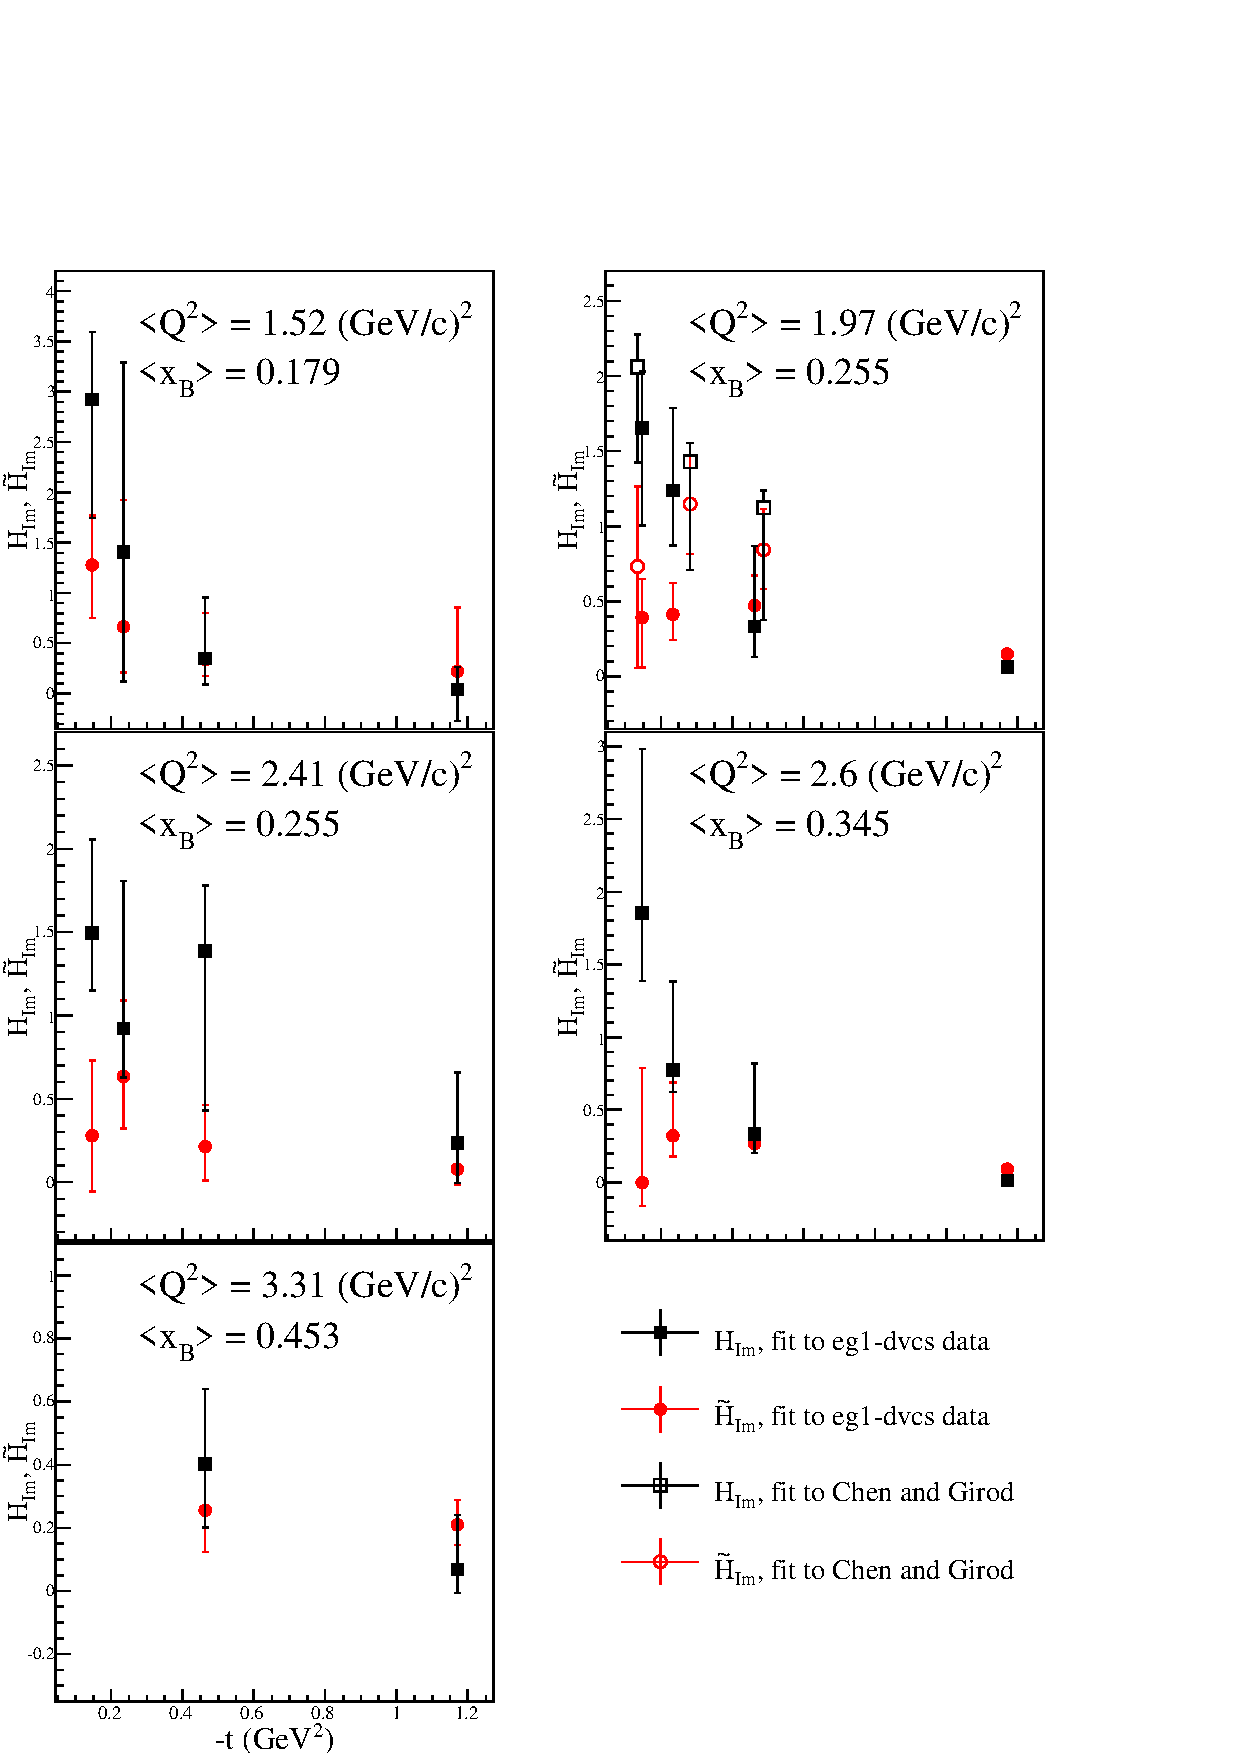
\includegraphics[width=120mm]{CFF_comp_prop.pdf}
\caption[$t$ dependence of $H_{lm}$ and $\tilde{H}_{lm}$.]
{$t$ dependence for each $Q^2$-$x_B$ bin of $H_{Im}$ (black squares) and $\tilde{H}_{Im}$ (red circles). The full points are obtained by fitting the eg1-DVCS data (TSA, BSA and DSA) \cite{pisano}. The empty points were obtained by fitting the BSA results from \cite{fx} integrated over all values of $Q^2$ at $x_B \sim 0.25$, and the TSAs from \cite{shifeng}.}
\label{cffs_eg1dvcs}
\end{center}
\end{figure}

\input{Exp_situation}
\input{Setup}

\subsection{Polarized target}\label{poltar-section}
\begin{figure}
\begin{center}
\includegraphics[width=5.5in]{Target_Side.pdf}
\end{center}
\caption{Side view of the CLAS12 dynamically polarized target.}
\label{Target}
\end{figure}
The proposed experiment will utilize a new, dynamically polarized target under construction for the CLAS12 spectrometer by a collaboration of the Jefferson Lab Target Group, the University of Virgina, Old Dominion University and Christopher Newport University.  The target cryostat, shown schematically in Figure~\ref{Target}, is specifically designed according to the geometrical constraints imposed by the CLAS12 detector package, primarily the Silicon Vertex Tracker.  Frozen, deuterated ammonia has been chosen as the target material for its high deuteron content (30\% by weight), high deuteron polarization (up to 50\%), and high resistance to radiation damage \cite{Goertz2002}.  Construction of the target is currently underway, with initial tests anticipated in 2017.

To realize Dynamic Nuclear Polarization (DNP), a dielectric solid is doped with a small concentration 
($10^{19}$~cm$^{\minus3}$) of paramagnetic radicals.  The unpaired electrons in the radicals are highly polarized by cooling the sample to a low temperature and applying a strong magnetic field.  For example, at the proposed operating conditions of 1~K and 5~T, the electron polarization is greater than 99.99\%.  Off-center microwave saturation of the electron spin resonance drives mutual electron/nuclear spin flips which effectively transfer the electron polarization to the nuclei.  Either positive or negative nuclear polarization can be realized, depending on whether the microwave frequency is slightly below or above the electron resonance frequency of 140~GHz.

The target sample will be cooled to 1~K by a bespoke $^4$He evaporation refrigerator with an anticipated cooling power of about 0.5~W at 1.0~K.  The CLAS12 solenoid shall provide the necessary 5~T magnetic field.  For optimum polarization, the uniformity of the field should be about 100 ppm or better over the volume of the sample.  If the solenoid is unable to provide this level of uniformity, it may be necessary to include small superconducting correction
coils inside the target cryostat, or to reduce the sample dimensions.  

\subsubsection{Luminosity}\label{sec_luminosity}
The nominal length of the target container will be $L=4.0$~cm, with a 2.5~cm diameter. 
It will be filled with mm-sized granules of frozen $^{14}$ND$_3$ with a density $\rho =$ 1.007 g/cm$^3$ and a packing fraction $f\approx0.6$.  The total luminosity with electron beam intensity $I$ will be 
\begin{eqnarray}
	\mathcal{L}  & = & f \rho L N_A I   \\
& = & 0.6(1.007\, {\rm g/cm}^3)(4.0\,{\rm cm})(6.02\times10^{23}\,{\rm g}^{\minus 1})(6.24\times10^9\,{\rm s}^{-1}{\rm nA}^{\minus 1}) \nonumber \\
	                   & = & 9.1 \times 10^{33} \, {\rm cm}^{\minus 2} \,{\rm s}^{\minus 1} \,{\rm nA}^{\minus 1} \nonumber
\end{eqnarray}
Note that this number is per nA of incident beam current.  
The luminosity for scattering from polarized neutrons
within the deuterons will be $3/20$ of the above number, or 
$1.4 \times 10^{33}\,{\rm cm}^{\minus 2} \, {\rm s}^{\minus 1} \, {\rm nA}^{\minus 1}$.
We anticipate running most of the experiment at 10~nA, giving a neutron luminosity of $1.4\times10^{34} 
\,{\rm cm}^{\minus 2} \, {\rm s}^{\minus 1}$.  An additional 10 days using the Forward Tagger will be run at a reduced beam current of 5~nA.  In order to reduce effects due to localized beam heating and radiation damage, the beam will be continuously rastered over 2.4~cm of the 2.5~cm target diameter.


\subsubsection{Polarization measurement}\label{sec_target_polarization}
The deuteron polarization will be monitored online by continuous wave NMR, using the industry standard
Liverpool Q-meter \cite{Court1993}.    There are two means whereby the polarization can be extracted from the NMR signal: the area method and the peak-height method.  We intend to use both, and either should provide a relative uncertainty $\Delta P/P \approx 4$\%.  We also intend to extract the polarization offline using the
quasi-elastic scattering asymmetry.

First, the total area of the NMR absorption signal is proportional to the vector polarization of the sample, and the constant of proportionality can be calibrated against the polarization of the sample measured under thermal equilibrium (TE) conditions.  This is the standard method used for polarized proton targets, but can be more problematic for deuteron targets.  Typical conditions for the TE measurements are 5~T and 1.4~K,
where the deuteron polarization is only 0.075\%, compared to 0.36\% for protons.
This smaller polarization, along with quadrupolar broadening, makes the deuteron TE signal more difficult to measure with high accuracy.
We therefore intend to implement a straightforward modification to the NMR circuit that has been shown to improve the stability and signal-to-noise ratio of the NMR signal~\cite{Court2004}. This modification was 
successfully utilized during the eg1-DVCS experiment in Hall B.  

Second, the deuteron polarization can also be extracted from the {\em shape\/} of the NMR signal.  
The deuteron is a spin-1 nucleus with three magnetic substates, $m=\minus1, 0, \plus1$, and the 
NMR absorption signal is a superposition of the $\minus 1-0$ and $\plus 1-0$ transitions.
In the case of ${}^{14}$ND$_3$, the deuteron's electric quadrupole moment interacts with electric field gradients within the molecule and splits the degeneracy of the two transitions.  The degree of splitting depends on the 
angle between the magnetic field and direction of the electric field gradient.  The resultant line shape, integrated over a sample of many polycrystalline beads, has the form of a Pake doublet (see Fig.\/\ref{NMR}).  
It has been experimentally demonstrated that, at or near steady-state conditions, the magnetic substates of deuterons in dynamically polarized ${}^{14}$ND$_3$ are populated according to the Boltzmann distribution with a characteristic {\em spin\/} temperature $T_s$ that can be either positive or negative, depending on the sign of the polarization. In this case, the vector polarization can be determined by the
ratio of the two transition intensities, $r=I_{\plus} / I_{\minus}$ \cite{Dulya1997}:
\begin{equation}
P_z = \frac{(r^2-1)}{(r^2 + r +1)}.
\end{equation}
An online estimate of the polarization can be made by comparing the heights of the two peaks.  
For a more accurate determination, an offline analysis of the entire line shape is necessary \cite{Dulya1997}.

\begin{figure}
\begin{center}
\includegraphics[width=3in]{Stache_NMR.pdf}
\end{center}
\caption[Typical ${}^{14}$ND$_3$ NMR signal]
{Typical NMR signal of polarized ${}^{14}$ND$_3$.  The black line results from a sophisticated line shape 
analysis of the data points and is a superposition of the two NMR transitions shown in red and blue.
This figure is adapted from~\cite{Kwaltine2013}.}
\label{NMR}
\end{figure}

Finally, the polarization will also be studied offline using the experimental data. We will extract the product of the beam and target polarization, $P_b P_t$, by measuring the quasi-elastic asymmetry ($\vec{d}(e,e'p)$) and by comparing it with the known theoretical value:
\begin{equation}
  P_b P_t=\frac{1}{D_f}\frac{A_{meas}}{A_{theo}}
\end{equation}
where $D_f$ is the dilution factor to account for the contribution of the unpolarized background (Section~\ref{sec_dilution}).
The target polarization value, needed for the TSA, will be then computed by taking the ratio of $P_bP_t$ and  the value of the beam polarization $P_t$, measured in dedicated M{\o}ller polarimetry runs. 

\subsubsection{Overhead for target operation}\label{sec_target_over}
There are four routine target operations that must be considered as overhead. 
First, we intend to provide an initial dose of approximately 20~Pe$^{\minus}$/cm$^2$ at 200~nA to each target sample prior to its use in the nDVCS experiment.\footnote{1 Pe$^{\minus} = 10^{15}$ electrons.}  This is necessary to achieve the highest possible deuteron polarization, as is explained below.  Second, the target must be periodically warmed to approximately 100~K in order to repair the deleterious effects of radiation damage, a process known as annealing.  Third, the target sample must be replaced when the anneals become ineffective at repairing the radiation damage.  Fourth, the NMR system will be periodically calibrated by performing
measurements of the thermal equilibrium polarization of deuterons at 5~T and temperatures around 1.4~K.
We examine each of these in the following sections, and a summary is made at the end.
Note that most overhead operations do not require the CEBAF electron beam, and are 
therefore counted as calendar days, not PAC days (one calendar day = two PAC days).
The only exception is the initial cold dose of electrons, as described below. Please note that this overhead estimate is for the total 110 days of beam time, consisting of 50 already-approved days and the additional 60 requested in this proposal. The target overhead is about the same for each. 

\vspace{-.15in}
\paragraph{Cold dose:}
In solid ammonia, paramagnetic radicals are created within the target sample by ionizing radiation, usually 
in the form of a 10--20~MeV electron beam, at a dose of about 
100~Pe$^{\minus}$/cm$^2$.
This is usually applied with the material cooled to 90~K with liquid argon, after which it may be stored indefinitely in liquid nitrogen.  
In the case of {\em deuterated\/} ammonia, experience has shown that polarizations greater than 20\% are only achieved after an additional  ``cold'' dose of approximately 10~Pe$^{\minus}$/cm$^2$ 
has been applied to the sample at 1~K.  
During the EG4 program in Hall B, the deuteron polarization increased from an initial value under 20\% to more than 45\%  after a cold dose of  20~Pe$^{\minus}$/cm$^2$~\cite{Slifer2007}.  In this case, the CLAS detectors were turned off and a 100~nA beam was applied to the sample for an hour or so, followed by a 100~K anneal.  These cold irradiations were interspersed with normal data-taking at 2~nA, and the deuteron polarization was observed to increase after each anneal, eventually exceeding 45\%.  Rather than following this prescription, we intend to prepare each target sample with a 20~Pe$^{\minus}$/cm$^2$ cold dose before using it in the experiment.  The CLAS12 detectors will be turned off for this procedure, which will require about a day for each sample at 200~nA. 

\vspace{-.15in}
\paragraph{Annealing:}
As a solid polarized target material, deuterated ammonia has a remarkably high resistance to radiation damage, 
exceeded only by lithium hydride and lithium deuteride.
When exposed to ionizing radiation, the decay of the polarization is roughly exponential in manner,
\begin{equation}
  P = P_o e^{-D/\delta}.
\end{equation}
Here $D$ is the dose, measured in Pe$^{\minus}$/cm$^2$.
The critical dose $\delta$ of ND$_3$ is different for the positive and negative spin states, with
$\delta_{\plus} = 13$~Pe$^{\minus}$/cm$^2$ and
$\delta_{\minus} = 26$~Pe$^{\minus}$/cm$^2$~\cite{Goertz2002}.
The polarization decay is due to the creation of additional paramagnetic species
that do not contribute directly to the DNP process, but do contribute to the spin-lattice 
relaxation of the nuclear spins.
Fortunately, the concentration of these new radicals can be reduced by annealing the target sample at temperatures up to about 100~K for some tens of minutes.

For the purposes of this proposal, we assume an initial polarization of 45\%, 
which has been achieved in both the Hall C polarized target and the original Hall B
polarized target.  To maintain an average polarization of 40\%, the radiation 
damage must be repaired by annealing the target sample when the polarization 
falls to 35\%, or in other words, when the dose reaches 
$\minus \ln(\frac{0.35}{0.45})\delta \approx 5$~Pe$^{\minus}$/cm$^2$.  
Here we have used the average value of $\delta_{\plus}$ and $\delta_{\minus}$.  
Assuming a 10~nA beam current distributed evenly over a 2.4~cm diameter, 
this dose will be accumulated, on average, after 4 days.  We estimate a total of four
hours will be required to anneal the target, cool it back to 1~K, and repolarize it to 40--45\%.

\vspace{-.15in}
\paragraph{Target lifetime:}
During 100 days of beam time at 10~nA, the polarized target
will accumulate a total dose of 120~Pe$^-$/cm$^2$, while an additional 10 days at 5~nA will deposit
6~Pe$^-$/cm$^2$.
However, the maximum that a ND$3$ sample can tolerate before it must be replaced is not fully known.  
McKee~\cite{McKee2004} reports that for the Gen01 experiment in Hall C, a total of dose of
315~Pe$^{\minus}$/cm$^2$ was deposited on six different samples, and at least one continued to give high polarizations even after a dose of 100~Pe$^{\minus}$/cm$^2$.  The total dose had little or no effect on the frequency of anneals, although the maximum attainable polarization did decline slightly after about 
50~Pe$^{\minus}$/cm$^2$.   For this proposal we make the conservative estimate that the samples will be replaced after a total dose of 50~Pe$^{\minus}$/cm$^2$, of which 20~Pe$^{\minus}$/cm$^2$
will occur before data-taking begins.  The remainder will be incurred after about
25~days of data-taking at 10~nA, and so we anticipate that four samples of ND$_3$ will be sufficient 
for the entire experiment, with one sample incurring an additional 6~Pe$^-$/cm$^2$ 
for the Forward Tagger runs.  Dedicated carbon runs will occur between the ND$_3$ sample changes.
The time required to replace an old ND$_3$ sample with the carbon target, then replace the carbon with fresh
ND$_3$, perform a TE calibration on the new sample and polarize it to 40--45\% should be about 12 hours. Note that this does not include the actual time spent acquiring data on the carbon target.

\vspace{-.15in}
\paragraph{TE measurements:}
Thermal equilibrium (TE) measurements are necessary to calibrate the NMR system,
and must be performed whenever a new target sample is introduced into the experiment.  Additional
measurements are made throughout the experiment in order to monitor and reduce sources of systematic uncertainty such as gain drift and settling of the sample beads.   
To perform a TE, the target sample must first have its existing dynamic polarization destroyed, either by temporarily warming the sample or temporarily lowering the magnetic field to zero.  The sample must then be allowed to achieve its thermal equilibrium polarization, which it approaches in an exponential manner with a spin-lattice time constant $T_1$ that depends on the field strength, the sample's temperature, and its density of paramagnetic radicals. Since annealing the sample reduces its radical density and increases $T_1$, 
it is best to do TEs prior to the anneals.  Most measurements are made around 1.4~K, where the signal size is not too small, and $T_1$ is not too long.
Because the deuteron TE signal is small, a significant amount of signal averaging must be utilized to achieve a precise determination of its area, and so the time required for each measurement will depend strongly on the signal-to-noise ratio of NMR system.  Based on past experience, we assume six hours will be sufficient.  This includes the time required to polarize the sample to 40-45\% at the end of the calibration.

\vspace{-.15in}
\paragraph{Target overhead summary:}
Based on the above information we provide the following estimate for the total overhead necessary to operate the polarized target.  The total is about 8 PAC days.  Whenever possible, anneals, TE measurements, and target changes can be coordinated with scheduled or unscheduled beam outages to lessen their impact on data acquisition and further reduce the overhead.  
%One possible sequence is indicated in Fig.~\ref{Operation}.
%\begin{figure}[ht]
%\begin{center}
%includegraphics[width=5.in]{Operation.pdf}
%\end{center}
%\caption[Possible target operation sequence]
%{One possible sequence of target operations for the 80 day experiment. The numbers indicate the total dose accumulated during data taking, in Pe$^-$/cm$^2$. The experiment ends after 95~Pe$^-$/cm$^2$.
%{\bf CD}: Cold Dose.  {\bf TE}: Thermal Equilibrium measurement.  {\bf A}: Anneal. }
%\label{Operation}
%\end{figure}
\begin{enumerate}
  \item{Cold dose of 20~Pe$^{\minus}$/cm$^2$ at 200~nA.  Required: 4 @ 24 hours each. 
    Total: 96 PAC hours.}  
    \item{Anneal every 5~Pe$^{\minus}$/cm$^2$.  Required: 22 @ 4 hours each. 
      Total: 88 calendar hours = 44 PAC hours.}
      \item{Change target sample after 30~Pe$^{\minus}$/cm$^2$.  Required: 3 @ 12 hours each.  
      Total: 36 calendar hours = 18 PAC hours.}
        \item{TE calibration of NMR system at the beginning of each target sample, and after 
          15~Pe$^{\minus}$/cm$^2$.  Required: 12 @ 6 hours each.  
          Total: 72 calendar hours = 36 PAC hours}.
\end{enumerate}

\begin{figure}
\begin{center}
\includegraphics[width=6in]{Operation_110days.pdf}
\end{center}
\caption[Overhead operations of the target]
{One possible sequence of target operations for the entire 110-day experiment. The top half represents the 50 days of already-approved beam time, and the bottom half the 60 days of extension. The numbers indicate the total dose accumulated during data taking, in Pe$^-$/cm$^2$. The experiment ends after 126 Pe$^-$/cm$^2$. 
{\bf CD:} Cold Dose. {\bf TE:} Thermal Equilibrium measurement. {\bf A:} Anneal.}
\label{Operation}
\end{figure}


\subsection{Central Neutron Detector}\label{cnd-section}
The Central Neutron Detector was conceived to extend the CLAS12 acceptance for the recoil neutrons of nDVCS, which are expected to be mostly emitted between $50^{\circ}$ and $70^{\circ}$ \cite{proposal}. The requirements of the detector are:
\begin{itemize}
\item{good capabilities for neutron identification, via the measurement of $\beta$ (with $\beta=\frac{v}{c}$), for the kinematic range of interest ($0.2<p_n<1.2$ GeV/c, $40^o<\theta_n<80^o$)} and
\item{neutron momentum resolution $\sigma_P/P$ within 10\%,}
\end{itemize}
Early simulation studies \cite{proposal} showed that these performances can be achieved by a scintillator-based detector providing a timing resolution of about 150 ps. 

\begin{figure}[ht]
\begin{center}
\includegraphics[width=3.5in]{CND_bello.pdf}
\end{center}
\caption [Design of the Central Neutron Detector]
{Design of the Central Neutron Detector, inserted in the CLAS12 solenoid.}
\label{cnd_nice}
\end{figure}

The core of the CND (Fig.~\ref{cnd_nice}), which will be placed in the Central Detector, in the 10 cm of radial space left between the Central Time Of Flight (CTOF) and the solenoid magnet, is a barrel, coaxial with the beam direction, made of three radial layers of trapezoidal plastic-scintillator bars. 
Each radial layer contains 48 bars, connected in pairs by a "u-turn" light guide at the downstream end.
Photomultipliers are coupled to the upstream end of each scintillator via 1.5m-long light guides. For each hit, half of the light emitted in a scintillator paddle is collected by the upstream PMT (the ``direct'' signal), while the other half propagates through the u-turn and the neighboring paddle to the PMT connected at its end (the ``indirect'' signal). 

Three such scintillator pairs (inner, middle, and outer) are grouped together to form a single, radial "block".  The CND comprises 24 of these blocks, covering the entire azimuthal range (Fig.~\ref{CND_Orsay}).

\begin{figure}
\begin{center}
    \includegraphics[height=40mm]{block_tested_2.pdf}
    \includegraphics[height=40mm]{cnd_finito.jpg}
  \caption{Construction and testing of the CND at Orsay. Left: one 2x3 block undergoing cosmic ray tests.  Right: all 24 blocks installed into a mock-up of the CLAS12 solenoid.}
  \label{CND_Orsay}
\end{center}
\end{figure}
The assembly of the CND, which was entirely carried out at the IPN Orsay, started in December 2013, and was completed in February 2015. The detector was shipped and stored at JLab in June 2015, awating its installation in CLAS12. Upon assembly, each block of the CND was tested with cosmic rays, triggering on the triple-coincidence of the signal in all three layers. Data were taken for about one week for each block, and the block performances were studied, with special attention to the timing resolution. 
Figure~\ref{tdc_adc_raw} shows the raw distribution of TDCs as a function of ADCs for the six PMTs in one of the 24 blocks. Notice the clear separation between direct (low-TDC/high-ADC) and indirect (high-TDC/low-ADC) signals. 

To define an average time resolution for our setup in the triple-coincidence trigger configuration, we use the method inspired by the work done in \cite{giles} and later adopted for the CLAS TOF system \cite{elton_paper}. 

\begin{figure}
\begin{center}
\includegraphics[width=140mm]{tdc_adc_raw.pdf}
\caption[Cosmic ray data for the CND]
{Cosmic rays data. Raw TDC vs ADC for each of the six PMTs of block 2 of the CND. No pedestal subtraction or data-cleaning cuts are applied.}
\label{tdc_adc_raw}
\end{center}
\end{figure}

\begin{figure}
\begin{center}
\includegraphics[width=80mm]{res_blocks.pdf}
\caption[Time resolution of the CND]
{Average time resolution for each block of the CND from cosmic rays measurements in triple-coincidence. The black and red triangles are the results obtained with the formulae from, respectively, Refs.~\cite{elton_paper} and \cite{vitali}.}
\label{res_blocks}
\end{center}
\end{figure}

The timing resolutions for all the CND blocks, computed according to the method of \cite{elton_paper}, are represented by the black triangles in Fig.~\ref{res_blocks}. The average is 148.0 ps. As a cross check, the resolution was also computed using the method adopted by V. Baturin for the CLAS12 CTOF \cite{vitali} (red triangles in Fig.~\ref{res_blocks}, with average 149.3 ps). The results of the two methods are consistent. The resolutions of the 24 blocks are very close to the required 150 ps. The systematic uncertainty of our results is estimated to be about $7\%$, determined by repeating the measurements multiple times, and by comparing multiple subsets of each measurement. 

Thus, for resolutions of 150 ps, we have a systematic uncertainty of about 10 ps.

It is also worth mentioning that the TDCs that will be used for the actual experiment will have a better resolution (25ps/channel) than the ones used for these tests (50ps/channel).

\subsection{Simulation and reconstruction}\label{sim_sec}
\begin{figure}[htb]
\begin{center}
\includegraphics[width=80mm]{CND_4.pdf}
%\vspace{-3.5cm}
\caption {Geometry of the Central Neutron Detector in the GEMC simulation, showing three layers of scintillator paddles (green) coupled in pairs via u-turn light guides (blue) downstream.}
\label{cnd_gemc}
\end{center}
\end{figure}

In order to study the performances of this detector, and thus evaluate the projected results of the nDVCS experiment, its geometry (Fig.~\ref{cnd_gemc}) has been added to the CLAS12 GEANT4-based simulation package, GEMC \cite{mauri}. The energy loss of the particle in the scintillator material is converted to numbers of optical photons in accordance with Birk's formula \cite{birks}, the resulting signal is propagated through the scintillator paddle, light guide and PMT, and the final charge and time are digitized to mimic the output from the ADC/TDC \cite{daria_wiki}.

The timing resolution and the energy loss due to the u-turn geometry have been included in the simulation using the values measured in the cosmic-rays tests described in the previous section. 

Simulations, which included all the other components of the Central Detector, have been run to evaluate the efficiency of the CND for neutrons, its ability to discriminate between neutrons and photons, and its angular and momentum resolutions. Neutrons and photons of momenta varying between 0.1 and 1 GeV/c and having polar angles $\theta$ varying between $50^o$ and $70^o$ have been generated at fixed azimuthal angle ($\phi = 0^o$), pointing to the center of one of the scintillator bars. The results obtained with these simulations are described here below..

\subsubsection{Efficiency}\label{efficiency-section}

 The detection efficiency is defined here as the ratio between the number of events for which a good hit (i.e., a hit having deposited energy above a given threshold) was successfully reconstructed as a neutron in the correct azimuthal bin of the CND and the total number of neutrons generated. 
Several values of energy thresholds, between 1 and 5 MeV, have been tested. 
The efficiency decreases with increasing threshold, and ranges between 12\% at the lowest thresholds and 7\% at the highest ones. 
Figure~\ref{eff_vs_mom} shows the efficiency as a function of the momentum of the neutrons, at a fixed energy threshold of 2 MeV, and for different values of $\theta_n$. 

\begin{figure}[t]  
\begin{center}
\includegraphics[width=100mm]{eff_vs_mom_diff_theta_II.pdf}
\caption [Neutron detection efficiency as a function of neutron momentum]
{Efficiency for the detection of neutrons, as a function of neutron momentum, for a 2-MeV threshold on the deposited energy. The efficiency is shown for three different values of $\theta_n$, between $50^o$ and $70^o$.
}
\label{eff_vs_mom}
\end{center}
\end{figure}

\subsubsection{Angular and momentum resolutions}\label{resolution-section}

The resolutions on the polar angle $\theta$ of the neutron that can be obtained with the CND are strongly linked to its TOF resolution. The angle $\theta$ is in fact given by
\begin{eqnarray} 
\theta = (180/\pi)\cdot \arccos (\frac{z_{ave}}{l})
\end{eqnarray}
where the reconstructions of the radial distance of the hit from the target, $l$, and of its position along the scintillator bar, $z_{ave}$,  both depend on the time measurement. Using a value deduced from the measurements on the CND prototype to apply a gaussian smearing on the timing \cite{proposal}, 
%\begin{equation}\label{eq_time_smear}
%\sigma_t=\frac{A}{\sqrt{E_{dep}}}, 
%\end{equation}
%(see Appendix~\ref{sec_rec})
the $\theta$ resolution resulting from GEMC was studied as a function of neutron momentum and $\theta$ itself. The results are shown in Fig.~\ref{theta_n_tofcut5}, where the angular resolution $\sigma_\theta$, obtained via gaussian fits of the simulated $\theta$ distributions, is plotted as a function of  $\theta$, for a particular value of neutron momentum (0.4 GeV/c). $\sigma_\theta$ is seen to increase slightly with the angle, from $1.5^{\circ}$ to $3.5^{\circ}$.  It has also been found to be relatively insensitive to the neutron momentum. 

The resolution on the azimuthal angle is directly connected to the total number of scintillator bars along $\phi$. In fact, the bin size $\Delta\phi$ is given by
\begin{eqnarray} 
\Delta\phi = \frac{360^{\circ}}{N}=7.5^{\circ}
\end{eqnarray}
where $N$ is the total number of paddles in $\phi$ (48 for the final design of the CND). $\sigma_\phi$ can be taken as half of $\Delta\phi$, therefore $3.75^o$.
\begin{figure}[hbt]  
\begin{center}
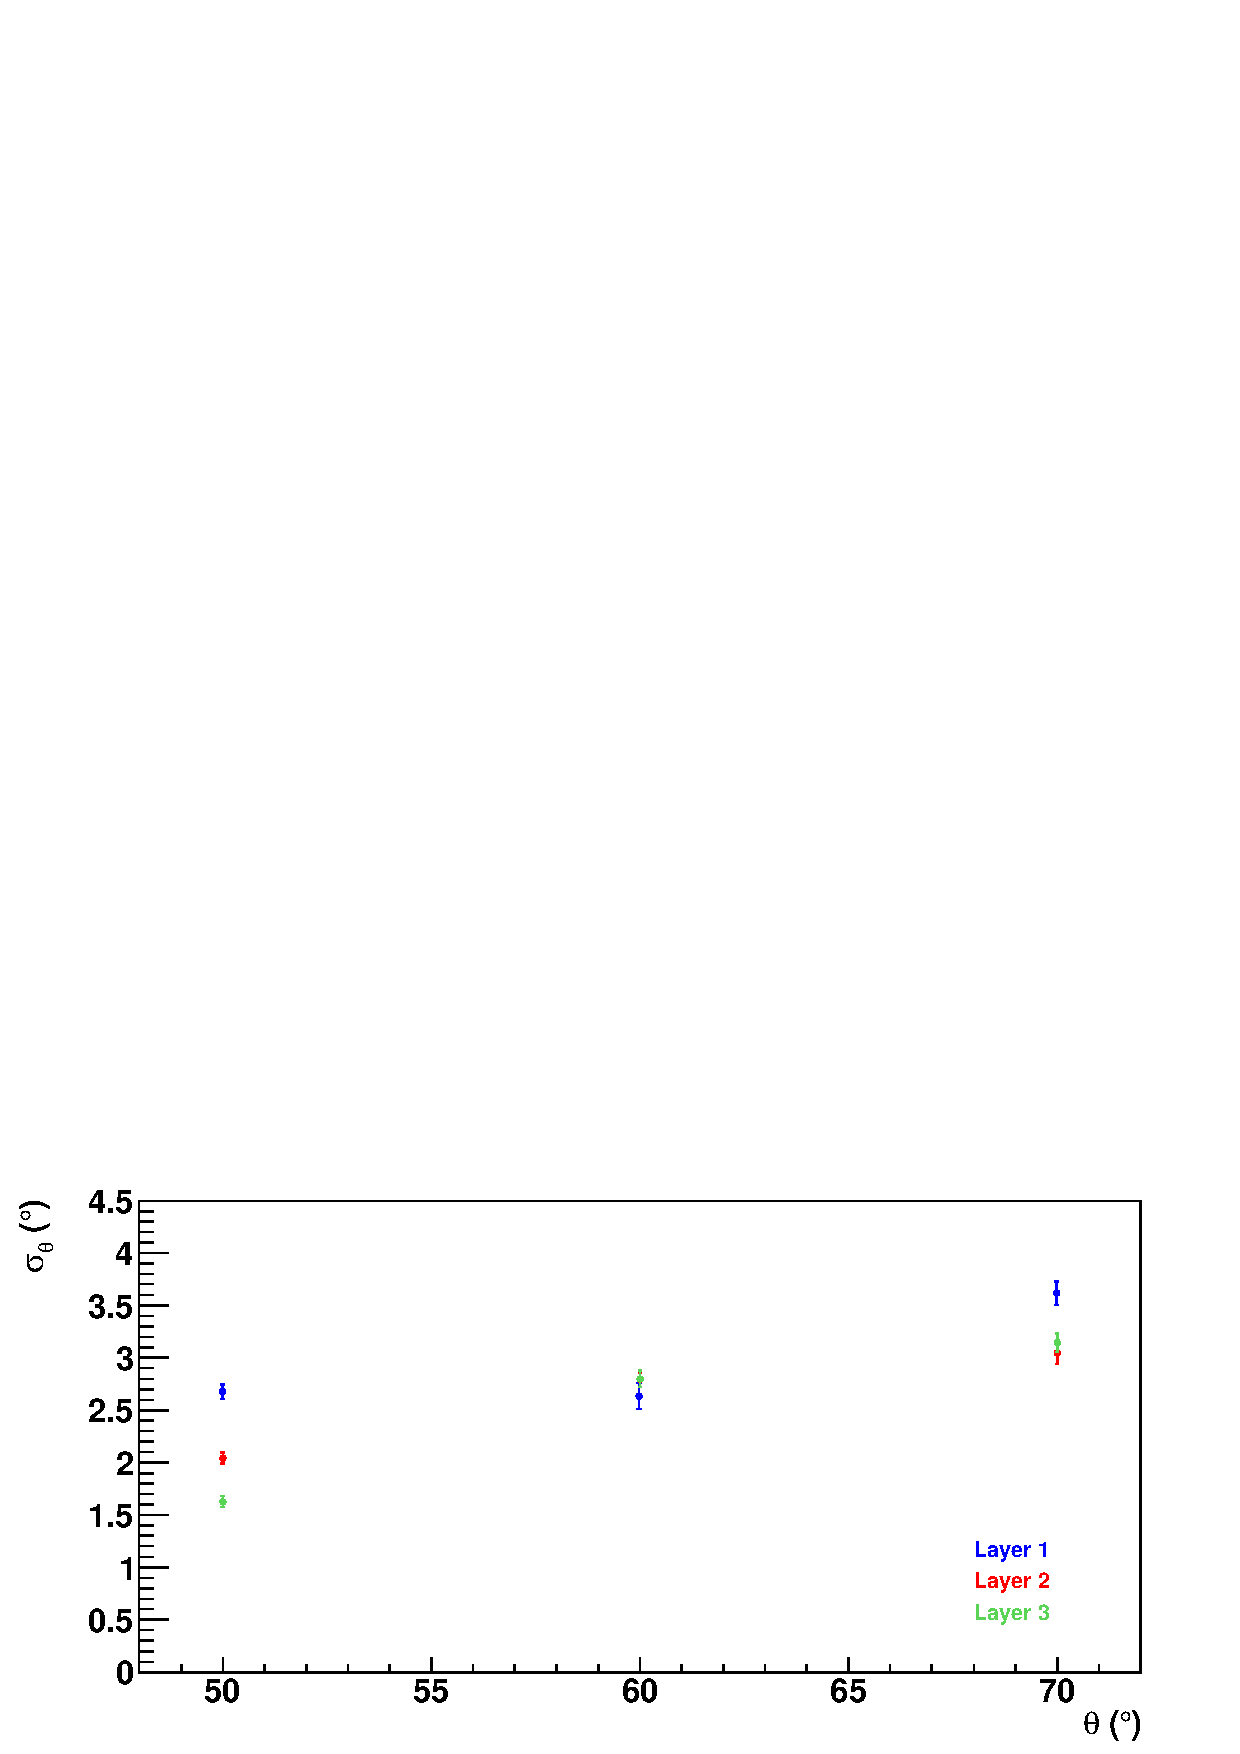
\includegraphics[width=100mm]{sigma_theta_vs_theta_diff_layer.pdf}
\caption [Angular resolution of the CND as a function of $\theta$]
{Angular resolution $\sigma_\theta$ as a function of $\theta$ for neutrons of momentum 0.4 GeV/c, for a 2-MeV threshold on the deposited energy. The three colors of the points correspond to the three radial layers of the CND.}
\label{theta_n_tofcut5}
\end{center}
\end{figure}

\begin{figure}  
\begin{center}
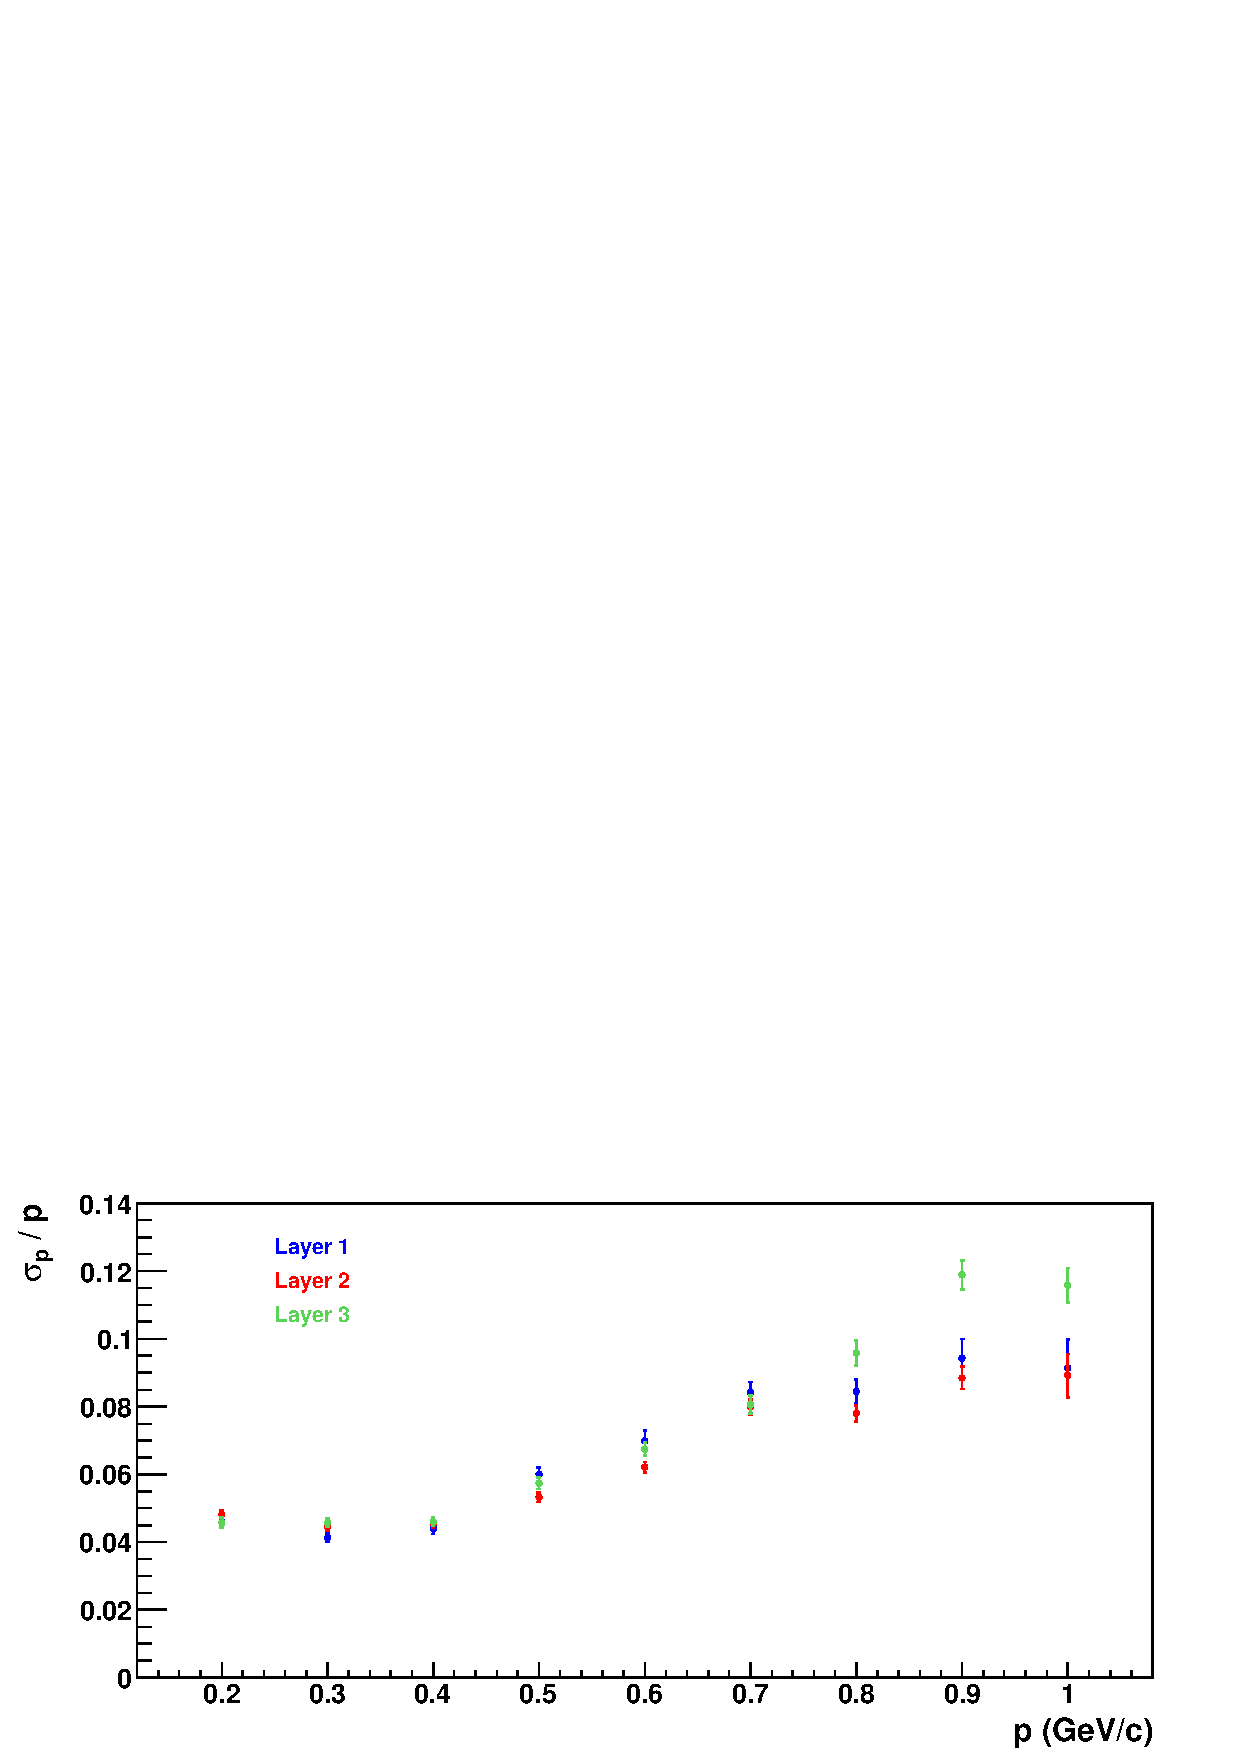
\includegraphics[width=100mm]{mom_res_vs_mom_diff_layers.pdf}
\caption [Momentum resolution as a function of $p$]
{Momentum resolution $\sigma_p/p$ as a function of $p$ for neutrons having $\theta=60^o$, for a 2-MeV threshold on the deposited energy. The three colors of the points correspond to the three radial layers of the CND.}
\label{p_n_tofcut5}
\end{center}
\end{figure}

The resolution on the neutron momentum, calculated after particle identification on the basis of $\beta$, according to the formula
\begin{eqnarray}
p = \frac{\beta\cdot m_n}{\sqrt{1-\beta^2}},
\end{eqnarray}
is also strictly connected to the TOF resolution. Figure \ref{p_n_tofcut5} shows the momentum resolution $\sigma_p/p$ as a function of momentum for neutrons emitted with $\theta=60^o$: it increases with increasing momentum, and ranges between 4\% and 11\%. No appreciable variations of momentum resolution are observed by varying the neutron polar angle.


\subsubsection{Particle Identification}\label{pid-section}

Since the charged particles passing through the CND will be vetoed by the Central Tracker, the only particles that could be mistaken for neutrons in the CND are the photons. 
The efficiency of the CND for detecting photons (Fig.~\ref{eff_photons}) has been estimated in simulations to be similar to that for neutrons, about 10\% for photon energies down to 0.2 GeV.  The efficiency drops to zero for lower energy photons, depending on the threshold cut applied. 

\begin{figure}  
\begin{center}
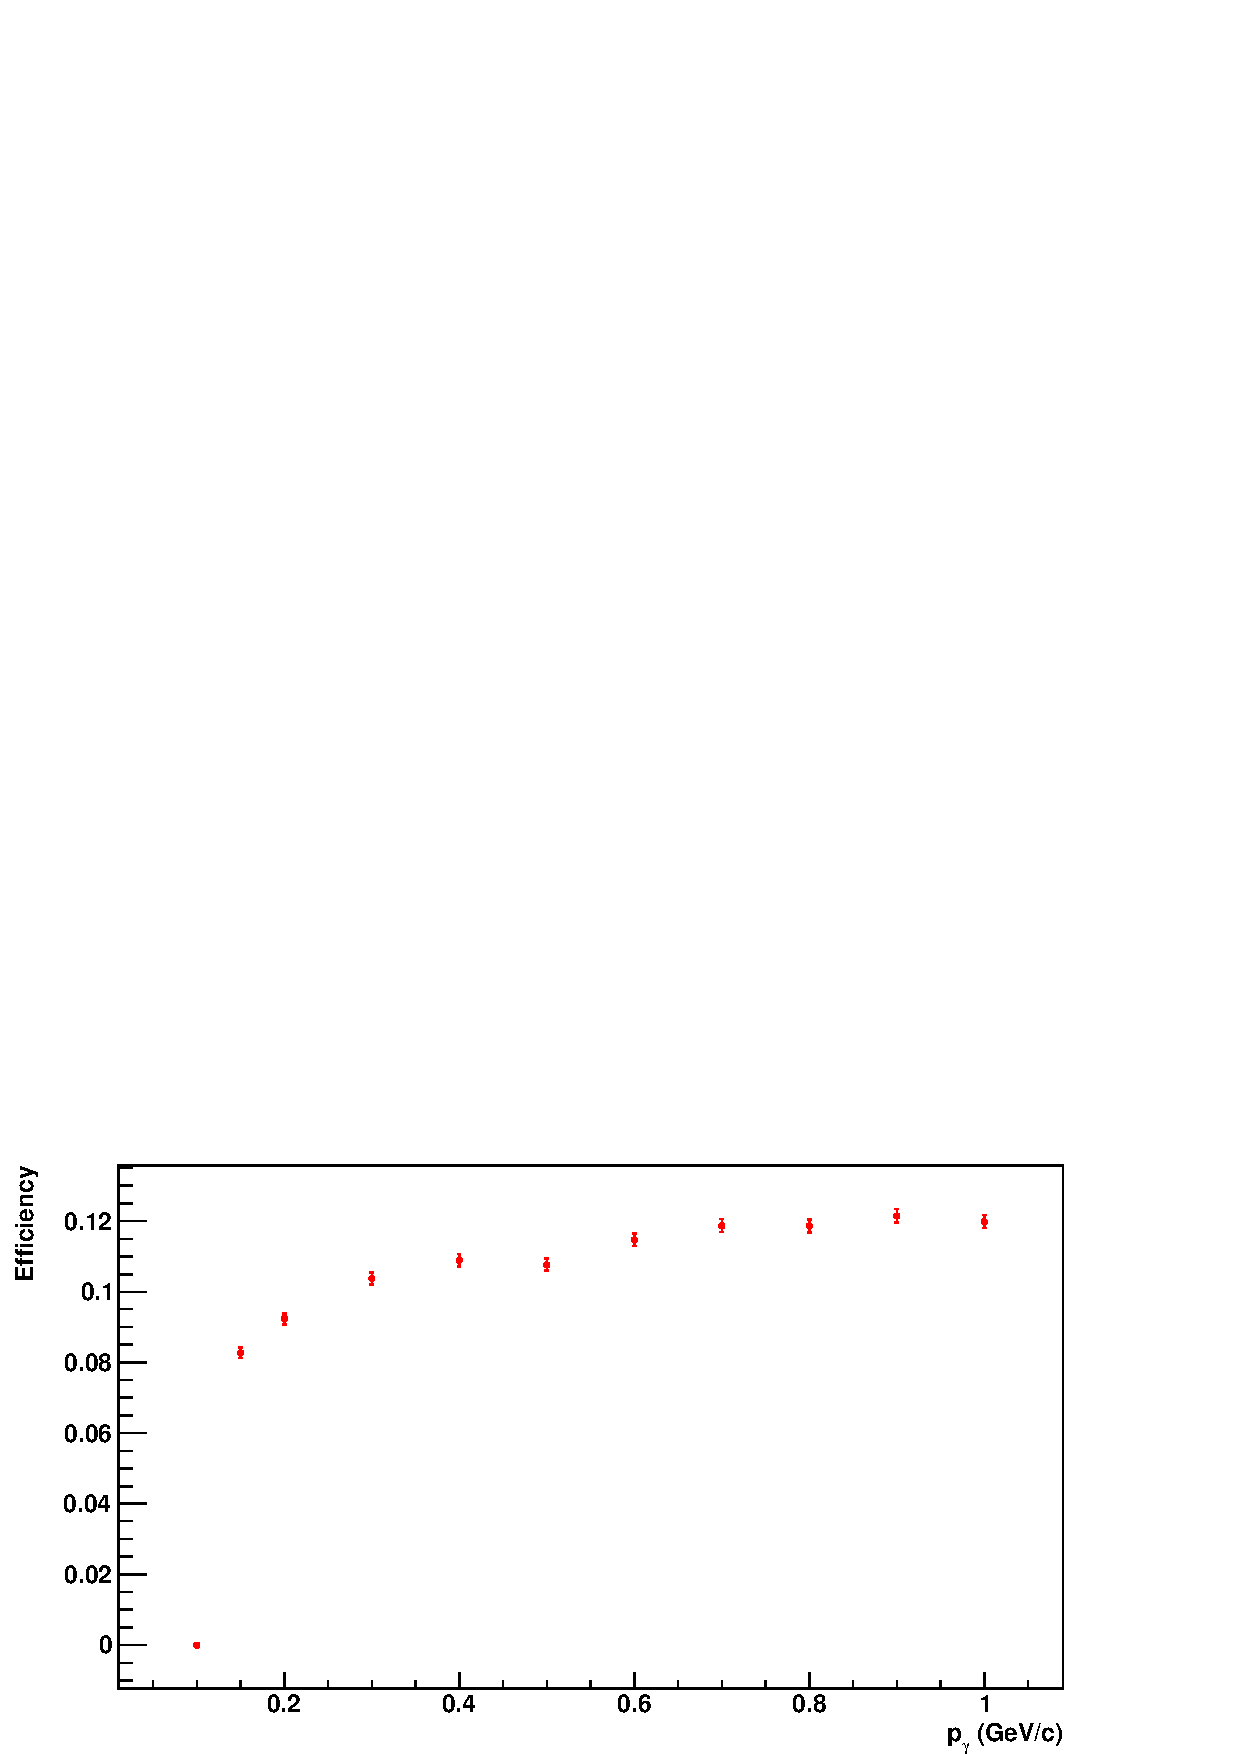
\includegraphics[width=100mm]{efficiency_photons_60deg_new.pdf}
\caption [Photon detection efficiency as a function of photon momentum]
{Efficiency for the detection of photons, as a function of photon momentum, for a 2-MeV threshold on the deposited energy. The efficiency is shown for $\theta_{\gamma}=60^o$. Below $E_\gamma=0.15$ GeV, the photon efficiency drops to zero.}
\label{eff_photons}
\end{center}
\end{figure}

\begin{figure}
\begin{center}
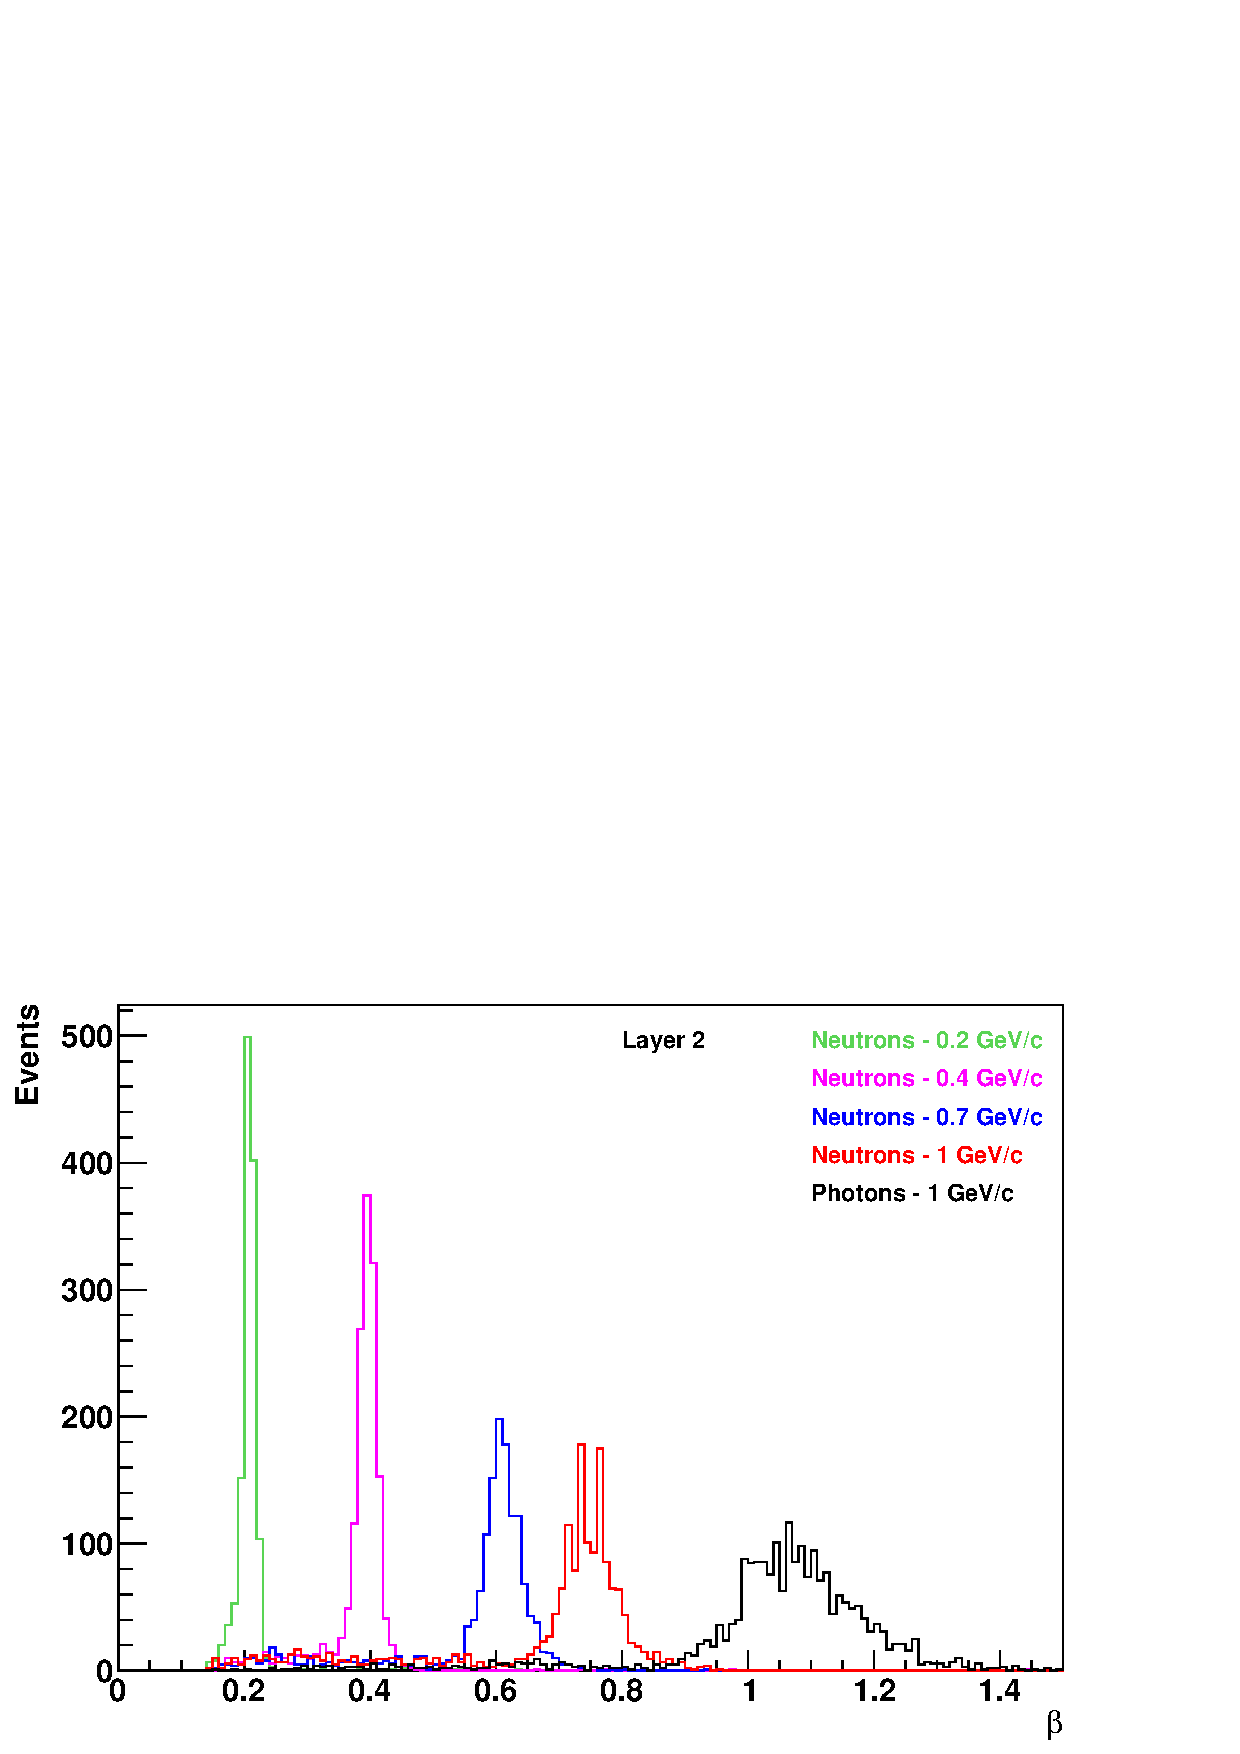
\includegraphics[width=80mm]{beta_comp_layer_2_II.pdf}
\caption [$\beta$ distributions for neutrons and photons in the CND]
{$\beta$ distributions for neutrons with $p_n=0.2$ GeV/c (green), $p_n=0.4$ GeV/c (purple), $p_n=0.7$ GeV/c (blue), $p_n=1$ GeV/c (red), and photons with $E=1$ GeV, for the middle layer of the CND. 
The threshold on the deposited energy is 2 MeV. The plots show all hits, integrated over $\phi$. Equal neutron and photon yields have been assumed here.}
\label{beta_n_g}
\end{center}
\end{figure}

\begin{figure}
\begin{center}
\includegraphics[width=100mm]{beta_res_n_g_comp_L2.pdf}
\caption [$\beta$ versus momentum for neutrons and photons in the CND]
{$\beta$ versus momentum for neutrons (red) and photons (blue) with momenta between 0.2 and 1 GeV, for the middle layer of the CND. The error bars are defined as $3\sigma$, where $\sigma$ is the fitted width of each $\beta$ peak. The threshold on the deposited energy is 2 MeV.}
\label{fig_beta_res}
\end{center}
\end{figure}

Neutrons can be discriminated from photons by means of their $\beta$, and so GEMC simulations have been performed to estimate the $\beta$ distributions that may be obtained from the CND.  Results for one of the three radial layers, integrated over the azimuthal angle, is shown in Figure~\ref{beta_n_g}.  Here $\beta$ distributions for neutrons with momenta between 0.2 and 1 GeV/c are compared with 1 GeV photons.  Very clear separation is evident for neutrons less than about 0.9 GeV/c, which comprise over 90\% of the expected nDVCS events. 

This is evident also from Fig.~\ref{fig_beta_res}, where the error bars correspond to $3 \sigma$, where $\sigma$ is the gaussian width of each $\beta$ distribution. Equal neutrons and photon yields have been assumed for this study. This assumption has been justified with detailed studies on the different types of photonic backgrounds that can affect the CND \cite{proposal}.

\input{Analysis}
\section{Projected results}\label{sec_countrate}
A GPD-based event generator for DVCS-BH on a deuterium target was run, assuming a luminosity of $3/20\cdot 10^{35}$ cm$^2$ s$^{-1}$ (where the factor $3/20$ accounts for the ratio of polarized neutrons to the total nucleons in ND$_3$) and a beam time of 100 days. The output of the generator was fed to the CLAS12 Fast-MC code, which included acceptance and resolution effects for CLAS12 and the CND. An additional factor of $10\%$ was also applied to mimick the efficiency of the CND for neutrons\footnote{Actually, this factor was adopted globally for ALL neutrons, even those falling within the EC acceptance. Given that the EC should have higher neutron efficiency than the CND, by at least a factor of 2, the projections for the count rates shown here are slightly pessimistic.}. nDVCS exclusivity cuts were then applied. This way, the expected yields for the $en\gamma(p)$ events produced on the ND$_3$ target were obtained. The kinematic space (in $Q^2$, $x_B$, $-t$, $\phi$) available with the acceptance of the CLAS12+CND setup was divided into the same 4-dimensional grid that was used for the unpolarized nDVCS proposal:
\begin{itemize}
\item{4 bins in $Q^2$, the limits of which are: 1, 2, 3.5, 5, 10 (GeV)$^2$;}
\item{4 bins in $x_B$, the limits of which are: 0.05, 0.15, 0.3, 0.45, 0.7;}
\item{4 bins in $-t$, the limits of which are: 0, 0.2, 0.5, 0.8, 1.2 (GeV)$^2$;}
\item{12 bins in $\phi$.}
\end{itemize}

The central kinematics for each bin were computed as weighted averages over the reconstructed events. The target-spin asymmetry and the double-spin asymmetry were then calculated as a function of $\phi$ using the VGG model (with input parameters $J_u=0.3$ and $J_d=0.1$) for each of the ($Q^2$, $x_B$, $-t$) bins that are kinematically allowed. 
Statistical errors were then obtained for these asymmetries using the approximated formula: 
\begin{equation}\label{error_asym}
\sigma_A = \frac{1}{P}\cdot \frac{\sqrt{1-P^2\cdot A^2}}{\sqrt{N}}.
\end{equation}
where $P$ is the polarization (and it is therefore equal to the target polarization for neutrons, $P_t$, for the TSA case, and to the product of beam and target polarizations, $P_bP_t$, for the DSA case), and $N$ is the expected yield in each 4-dimensional bin. % (Figs.~\ref{count_rate_1} and \ref{count_rate_2}). 

The resulting asymmetries with the associated expected error bars are shown in Figs.~\ref{fig_tsa_100_50_FT} (TSA) and \ref{fig_dsa_100_50_FT} (DSA). These same figures also show the comparison, for TSA and DSA, for running this experiment with either 50 or the proposed 110 days of beam time. 
The use of the Forward Tagger will improve the $\phi$ coverage at the edges ($\phi\to 0^{\circ}$ and $\phi\to 360^{\circ}$) for some of the low-$t$ bins, which is otherwise incomplete. This can be noticed in Figs.~\ref{fig_tsa_100_50_FT} and \ref{fig_dsa_100_50_FT}, where at the edges of several of the $\phi$ distributions only the black points are present. 

%For reference, the 4-dimensional acceptances obtained with the simulation are shown in Figs.~\ref{acceptance_1} and \ref{acceptance_2}. 

It is important to point out that the number of days chosen here (110) is the minimal amount of time necessary to be able to bin the TSA and the DSA in enough kinematic bins to describe in a satisfactory manner the dependence in all the 4 kinematic variables, while at the same time having statistical uncertainties not exceeding too much the ones expected for the BSA of E12-11-003 (Fig.~\ref{fig_bsa}). 

%\begin{sidewaysfigure}  
%\begin{center}
%\includegraphics[width=200mm]{asym_polndvcs_tsa_newvgg_100days_FT_noFT.pdf}
%\caption[Projected target-spin asymetry]
%{Projected target-spin asymmetry. The y-scale range, common to all bins, is (-1;1). The black and red points are obtained, respectively, without and with the Forward Tagger. }\label{fig_tsa}
%\end{center}
%\end{sidewaysfigure}

\begin{sidewaysfigure}  
\begin{center}
\includegraphics[width=200mm]{asym_polndvcs_tsa_newvgg_100_FT_and_noFT_50days.pdf}
\caption[Projected target-spin asymetry]
{Projected target-spin asymmetry. The y-scale range, common to all bins, is (-1;1). The black and red points are obtained, respectively, with 110 days and 50 days of beamtime.}\label{fig_tsa_100_50_FT}
\end{center}
\end{sidewaysfigure}

\begin{sidewaysfigure}  
\begin{center}
\includegraphics[width=200mm]{asym_polndvcs_dsa_newvgg_BH_100_50days_FT_and_noFT.pdf}
\caption[Projected double-spin asymmetry]
{Projected double-spin asymmetry, compared to the BH (green lines), calculated at the average kinematics of each bin. The y-scale range, common to all bins, is -0.6-1.2. The black and red points are obtained, respectively, with 110 days and 50 days of beamtime. }\label{fig_dsa_100_50_FT}
\end{center}
\end{sidewaysfigure}

\begin{sidewaysfigure}  
\begin{center}
\includegraphics[width=160mm]{asym_newcuts_bsa_newvgg.pdf}
\caption[Projected beam-spin asymmetry from E12-11-003]
{Projected beam-spin asymmetry, as will be obtained from experiment E12-11-003 \cite{proposal}. The y-scale range, common to all bins, is -0.25-0.25.}\label{fig_bsa}
\end{center}
\end{sidewaysfigure}

\input{CFF_Results}
\section{Systematic uncertainties}\label{sec_syst}
The goal of this experiment is to extract target and double-spin asymmetries, which are ratios of polarized cross sections. In the ratio, polarization-independent terms, such as acceptances, efficiencies, radiative corrections and luminosity, cancel out to a first approximation\footnote{Afanasev {\it et al.} \cite{afanasev} have computed the radiative corrections for the DVCS and BH processes on for CLAS kinematics. It was found that, given the strict kinematic cuts adopted to select the final state, the undetected radiated photon can only have small energies. In this case, therefore, the main contribution to the radiative correction comes from spin-independent soft-photon emission that does not affect the polarization observables. The approximation of negligible contribution from the radiative corrections to the BSA, TSA and DSA, compared to the size of the asymmetries, was estimated to be valid at the 0.1\% level \cite{afanasev}.}. Remaining effects could come from the quantities entering in the asymmetry definitions, namely the procedure to evaluate the counts $N^{+(-)}$, the dilution factor, the $\pi^0$ contamination, as well as the beam and target polarizations. 

Analyses performed at 6 GeV \cite{erin,pisano} showed that the biggest contributor to the overall systematic uncertainty is the selection of exclusivity cuts adopted to identify DVCS events and the corresponding counts $N^{+(-)}$. This factor contributed about 10\% (this and the following percentages for systematics are defined relatively to the average value of the TSA at $90^{\circ}$) to the total systematics uncertainty. 

Another source of uncertainty will be the $\pi^0$ background estimation, which will depend on the accuracy of the description of the detector acceptance and efficiency and on the model used in the Monte-Carlo simulation to describe the $en\pi^0(p)$ reaction (see Eq. 32). In order to account for this latter effect, 6-GeV analyses, performed on data taken on a polarized NH$_3$ target during the eg1-dvcs experiment \cite{erin,pisano}, evaluted this systematic by varying the contribution of the calculated background by $\pm 30\%$ (Section \ref{sec_pi0_back}), and extracting the final asymmetries in correspondence with this increased/decreased background. The total effect turned out to be 4\%, and a similar estimation can be assumed for the present experiment on ND$_3$.

While acceptance effects are expected to cancel in asymmetries, a residual effect could emerge due to the strong variations of the cross section inside the finite-size bins, that can lead, in principle, to a non-exact cancellation of acceptance effects from the numerator and the denominator. Such an acceptance effect has been estimated to bring an additional 1\% systematic error. 

To evaluate the systematic uncertainties linked to the dilution factor determination, in the aforementioned eg1-dvcs pDVCS analysis the  asymmetries were computed two more times, taking two different values of the dilution factor: $D_f+\Delta(D_f)$ and $D_f-\Delta(D_f)$, where $\Delta(D_f)$ is the statistical error that was estimated on this quantity. The resulting systematic uncertainties were found to be below the percent level. While studying the systematics on the exclusivity cuts, it was observed that changing the exclusivity cuts induces a variation of the dilution factors much bigger than the variations within the statistical errors described above. It was therefore decided, in order to avoid double-counting and therefore overestimation of systematics, to remove the contribution from the dilution factor computed according to its errors from the total systematic uncertainty. For this proposal, instead, a conservative estimate of the systematic uncertainty on the dilution factor of the order of 3\%, consistent with previous assumptions \cite{kuhn}, is assumed. 

%As for the systematic uncertainties on the dilution factors, in the aforementioned pDVCS 6-GeV analysis of eg1-dvcs were included in the exclusivity cut ones. Indeed, the systematic effect due to the variation of the exclusivity cuts represents the biggest contribution to the overall systematics, and, being the dilution factor strictly related to the specific set of exclusivity cuts adopted, its variation between the different sets of cuts turned out to be larger than its statistical error, making unnecessary a dedicated study.

An additional 2\% systematic effect is included in the total budget to account for the possible misidentification of neutrons due to accidental coincidences (Section~\ref{sec_accidentals}.)

Finally, uncertainties in the knowledge of the beam and target polarizations (extracted, respectively, via M{\o}ller polarimetry measurements and via the NMR system) will propagate into the asymmetry measurements, and are expected to lead to contributions of, respectively, 3\% and 4\%.

A summary of the systematic uncertainties can be found in Table~\ref{table_syst}. The total systematic uncertainty will be of the order of 12\%, averaged over all the kinematic bins (the $\pi^0$-background uncertainty will actually vary depending on the bin). 

\begin{table}
\begin{center}
\begin{tabular}{|c||c|}
\hline
Source of error & Systematic uncertainty\\
\hline
Channel selection cuts & 10\% \\
\hline
Beam and target polarization & 3\%-4\%  \\
\hline
$\pi^0$ contamination & 4\%  \\
\hline
Acceptance & 1\%  \\
\hline
Dilution factor & 3\%  \\
\hline
Accidentals & 2\%  \\
\hline
Radiative corrections & Negligible  \\
\hline
\hline
Total & 12\%  \\
\hline
\end{tabular}
\caption{Expected systematic uncertainties on the proposed measurement.}
\label{table_syst}
\end{center}
\end{table}

\input{Request}
\newpage
\chapter{DIS on Longitudinally Polarized Deuterium}
\centerline{Proposal to increase the beam time allocation for the ND$_3$ part}
\centerline{of Experiment 12-06-109 (approved by PAC 30 and rated ``A'' by PAC 36)}
\vskip 0.4cm
\centerline{Sebastian Kuhn\footnote{contact person, email: skuhn@odu.edu}}
\centerline{\it  Old Dominion University, Norfolk VA 23529}

\abstract
{We are proposing to add 50 more days of running to the 50 days already approved for the portion of Experiment 12-06-109 with CLAS12 and 11 GeV polarized electrons on longitudinally polarized deuterons (ND$_3$). This additional beam time (plus overhead and carbon runs) will significantly reduce the uncertainty on polarized parton distributions, in particular for $d$ quarks, in the limit of large $x$, as well as for gluons and the strange quark sea at moderate to large $x$. It will bring the deuteron data at least closer to parity with the already approved 120 days of data on the proton, thus maximizing the information that can be extracted from a single experiment, as well as making more significant comparisons with other experiments (e.g. on $^3$He) possible. This will be important to assess the impact of nuclear effects on the extraction of $\Delta d$ at high $x$, and to guarantee that the unique opportunity to finally map out the asymptotic behavior of all quark distributions provided by Jefferson Lab's 12 GeV beam will be optimally utilized. In this proposal, we are providing updated estimates of various quantities that can be extracted from these data under the assumption of a doubling for the integrated luminosity on the deuteron.
}
\newpage
\setcounter{page}{72}
\section{Introduction}

Experiment 12-06-109 (together with E12-09-007b) is a comprehensive program to map out the $x$- and $Q^2$-dependence of the helicity structure of the nucleon in the region of moderate to very large $x$. By collecting inclusive (DIS) and semi-inclusive (SIDIS) data over a wide kinematic range with CLAS12 and 11 GeV polarized electrons on both longitudinally polarized protons (NH$_3$) and deuterons (ND$_3$), this program aims to constrain global fits of polarized parton (quark and gluon) distributions, extract higher twist corrections to the DIS structure functions, and evaluate moments connected to local operators in the Operator Product Expansion (OPE). 
Experiment 12-06-109 was originally approved by PAC 30 (with a further review and scientific rating of ``A'' by PAC 36) for a total of 80 days, 30 days on NH$_3$ and 50 days on ND$_3$ (both including overhead).

In the meantime, additional experiments~\cite{RGC} on longitudinally polarized {\em protons} have been approved, with high rating. These experiments have brought the total number of PAC-approved days for the NH$_3$ target to 120 (run group Ca with CLAS12). 
In the meantime, the total runtime for the ND$_3$ target (run group Cb) has been largely unchanged (at present 65 days including all overhead for auxiliary measurements, target operations etc.). This discrepancy is even more striking when taking into account that ND$_3$ targets tend to have polarizations of roughly a factor 1/2 lower than NH$_3$ targets, resulting in an overall figure of merit (FoM) at least four times worse than for the proton. This means that any  analysis that requires information from both targets (e.g., global fits to extract polarized parton distributions) would have uncertainties that are totally dominated by the statistical error from the deuteron.

While some of the goals of the original experiment 12-06-109 can be reached with reasonable precision even with 50 PAC days on the deuteron, there are some physics observables whose precision would be ``statistics-starved'' under this scenario. In particular, the asymptotic behavior of the PDF $\Delta d$ at large $x$ would be much less constrained than what is possible with a doubling of the integrated luminosity. Deuteron data are also crucial to determine the total contribution from quark helicities to the nucleon spin ($\Delta \Sigma$), as well as polarized gluon and strange quark PDFs at moderate to large $x$ (see details in the following sections). Because of their smaller count rates, SIDIS channels will benefit significantly from additional statistics. As we lay out in detail in the following sections, a doubling of the actual run time on polarized ND$_3$ from 50 to 100 days (plus the necessary overhead) will optimize the overall physics output from Experiment 12-06-109 and maximize the return on the large investment in the spin physics program with Jefferson Lab at 12 GeV.
No other facility presently running or under construction will be able to probe, with comparable precision, the kinematic region of moderate to large $x$ and moderate $Q^2$ accessible here.

%The additional 10 days at 5 nA with the inclusion of the Forward Tagger, as requested in the nDVCS part of this proposal, will not directly impact the program of measuring collinear spin structure functions, and has not been included in the estimates that follow in this chapter. However, it offers the potential for measurements of spin structure functions at very low $Q^2$ (measuring the scattered electron in the FT), that are of interest in their own right, and as part of the radiative corrections for DIS. 

%To fully elucidate the spin structure of the nucleon in the valence region, one has to combine 
%information from many different experimental approaches. Both deeply virtual exclusive processes,
%which are sensitive to Generalized Parton Distributions (GPDs), and semi-inclusive processes (in particular
%those involving single spin asymmetries which are sensitive to Transverse Momentum-dependent Distributions - TMDs)
% will access some part of this puzzle. However, high precision
%measurements of structure functions (as well as of elastic form factors) remain indispensable, both to
%constrain the parameters of GPD and TMD fits, and as the most direct access to the longitudinal structure
%of the nucleon. In particular, spin structure functions of the nucleon in the valence region and at very large
%$x$ are still poorly known, in spite of their fundamental significance for tests of pQCD and models of
%nucleon structure. Jefferson Lab with 11-12 GeV beams is the unique place where this gap can be finally closed.
%The accessible kinematics is also uniquely suited to study the transition from partonic degrees of freedom
%to hadronic ones, through detailed measurements of higher twist operator matrix elements and a
%complete investigation of the phenomenon of quark-hadron duality in spin structure functions.

\subsection{The Deuteron and CLAS12}

A complete mapping of spin structure functions and the extraction, through global PDF fits, of polarized parton distributions require a complete set of measurements on both types of nucleons, protons and neutrons, over the widest possible range in $x$ and $Q^2$. 
In addition, since neutrons can only be accessed bound in nuclei, it is very important that both commonly used nuclear targets, $^3$He and deuterium, be studied with high precision, since nuclear effects and their uncertainties are very different for these two cases. Furthermore, the deuteron is the best substitute for a purely isoscalar nucleon target, which is ideal for extracting information on gluon and sea quark helicity distributions through NLO analyses. For these reasons, a high-statistics measurement on polarized deuterium (ND$_3$) is obligatory.

Presently, the only readily available and suitable targets for polarized protons and deuterons employ solid state compounds like ammonia, butanol or lithium deuteride at low ($\approx 1$ K) temperatures. 
These compounds are susceptible to radiation damage and beam heating, limiting severely the practically achievable luminosities. 
The upgraded CLAS12 detector will be a perfect match for these targets, since it
\begin{itemize}
\item is optimized for luminosities of 1-2$\cdot 10^{35}$ cm$^{-2}$ s$^{-1}$, within a factor of 2-4 of the practical limit of cryogenic ammonia targets, and compensates for this relatively low luminosity with its very large acceptance
\item already contains a solenoidal magnet which will provide the (typically 5 Tesla) field needed for dynamic nuclear polarization, thus minimizing the extra costs of a polarized target
\item covers a large angular range, including backwards angles, which allows us to simultaneously measure inclusive, semi-inclusive and tagged structure functions (with backward-going target remnants) over the full kinematic range of interest (while also collecting data for deeply virtual exclusive processes and single spin asymmetries).
\end{itemize}

Our group is leading the development of an optimized longitudinally polarized proton and deuteron target for CLAS12, and coordinates the run group C using these targets. Significant investments in this program have already been made, partially through an NSF MRI grant. No other experiment with this particular type of targets has been planned with similar kinematics, at Jefferson Lab or elsewhere. We believe that adding 50 more days of running, plus overhead, to the already established run group C (an overall increase by only 25\%) will yield an optimal return on this investment.

\section{Scientific Case and Recent Developments}

\begin{figure}[htb!]
\begin{center}
\includegraphics[width=6in]{dis/LT_all_groups.pdf}
\end{center}
\caption{\baselineskip 13pt \small
Compilation of recent  polarized PDF fits from various groups. This Figure is from the  JAM15 paper~\cite{JAM15}
(Fig. 17) where all references for these fits can be found.}
\label{NLOfits}
\end{figure}

Inclusive and flavor-tagged spin structure functions of the nucleon have been measured for  over three decades~\cite{Kuhn:2008sy}, beginning with the
experiments at SLAC~\cite{Alguard:1976bm} and the discovery of the famous ``spin puzzle'' by the 
EMC~\cite{EMCfinal}. The goal of these experiments is to determine, via next-to-leading-order DGLAP analyses, 
 the helicity-dependent distribution functions (PDFs)
 of valence and sea quarks as well as gluons, see Fig.~\ref{NLOfits}. Collinear spin structure functions can also be used to evaluate 
 moments that are related to nucleon axial current matrix elements (e.g., the overall contribution of quark helicities to the
 nucleon spin), and to test fundamental sum rules like the Bj\"orken sum rule~\cite{Bjorken:1968dy}. 
 Finally, measuring their dependence on the
 photon virtuality $Q^2$ allows us to determine higher twist contributions, matrix elements in the framework of the operator
 product expansion (OPE), and the transition from partonic (high $Q^2$) to hadronic (low $Q^2$) degrees of freedom,
 including duality and 
 tests of the Gerasimov-Drell-Hearn sum rule and its extensions in, e.g., Chiral perturbation theory (see
 discussion and references in~\cite{Kuhn:2008sy}).
 In the new era of three-dimensional mapping of the nucleon parton distributions, collinear spin structure functions
 serve both as a crucial constraint on GPDs and TMDs, and provide two of the four ingredients to the celebrated
 nucleon spin sum rule.
 
Within recent years, data from high-energy polarized proton collisions at 
RHIC~\cite{STAR_jet15,PHENIX_pi14,PHENIX_pi15,STAR_W14,PHENIX_W15} 
have constrained the contribution of gluon
and sea quark helicities at low to moderate $x \le 0.2$ to the nucleon spin. Further information has come from measurements
of open charm production~\cite{COMPASS_g13}. The most recent 
inclusive data from COMPASS~\cite{COMPASS16} extend our knowledge of spin structure functions to the lowest
$x$ and highest $Q^2$ yet. 
Meanwhile, the spin structure function program with Jefferson Lab's 6 GeV has been concluded and most results have been 
published. In particular, very precise data on proton, deuteron and $^3$He 
targets~\cite{eg1b-d,eg1b-p,eg1-dvcs,E06-014_A1,E06-014_d2,E01-012}
 have recently appeared 
that cover a large kinematic range, from low $Q^2$ to the DIS region. This program is being continued in the 12 GeV era, with several
experiments in three halls approved with scientific rating of ``A''. The unique importance of these expected Jefferson Lab 
data is threefold:

\begin{figure}[htb!]
\begin{center}
\includegraphics[width=6in]{dis/IMPACT_JLAB.pdf}
\end{center}
\caption{\baselineskip 13pt \small
Impact of recent Jefferson Lab data on the global NLO PDF fit by the Jefferson Lab Angular Momentum (JAM) collaboration. 
This Figure is from the recent JAM15 paper~\cite{JAM15}
(Fig. 15) where all relevant references  can be found. The l.h.s. fits are for the leading twist distributions for three quark flavors
and gluons, while the r.h.s. shows the results for various higher-twist terms.The yellow lines are from repeated
Monte Carlo fits including all world data except those from Jefferson Lab; the red lines include the Jefferson Lab data and
clearly have a much more narrow uncertainty band.}
\label{JLabImpact}
\end{figure}

\begin{enumerate}
\item For a DGLAP determination of all individual parton distribution functions, but in particular those of the gluon, from DIS data,
a large leverarm in $Q^2$ is required to exploit scaling violations. The recent precise data from COMPASS~\cite{COMPASS16}
cover the high-$Q^2$ limit\footnote{These will be greatly improved upon, both in kinematic reach and in precision, by data
to be acquired with the future EIC; however, the low-$Q^2$ data fromJefferson Lab will likely not be matched in the foreseeable future.},
 while precise data at the lowest $Q^2$ consistent with DIS come from Jefferson Lab. The latter cover 
a large range in $Q^2$, which in itself allows us to reliably extract and control for higher-twist effects. Figure~\ref{JLabImpact}
demonstrates the significant improvement in our knowledge of {\em all} polarized PDFs enabled already by the existing
Jefferson Lab data.

\begin{figure}[htb!]
\begin{center}
\includegraphics[width=4in]{dis/delqFig-eps-converted-to.pdf}
\end{center}
\vspace{-0.2in}
\caption{\baselineskip 13pt \small
$\Delta u/u$ (upper half) and $\Delta d/d$ (lower half) results from Jefferson Lab
Hall A and CLAS data (in leading order approximation), compared with other world data
and three different predictions: a fit by Leader, Stamenov and Siderov~\cite{Leader:2006xc} (black line), and two pQCD
predictions without~\cite{Brodsky:1994kg} (dashed)  and with~\cite{Avakian:2007xa} (solid red and blue lines)
inclusion of orbital angular momentum effects.  }
\label{highx}
\end{figure}

\item While the contribution from PDFs in the valence region $x > 0.3$ and, especially, in the limit $x \rightarrow 1$, to the overall
nucleon spin is not very large, knowledge of PDFs in this regime is crucial to understand the valence structure of the nucleon and to
test predictions from pQCD and various models. Only Jefferson Lab at 12 GeV can provide the necessary precision data
in these kinematics for the foreseeable future. In particular, the asymptotic polarization of d quarks in the proton,
$\Delta d/ d$ at large $x$, is presently poorly known (see Fig.~\ref{highx}), 
and a reliable measurement requires high statistics data from both
deuterons and $^3$He.

\item Beyond the leading-order PDFs, higher twist structure functions are of high current interest in themselves, since
they contain information about correlations and interactions between gluons and quarks in the nucleon. Again, only at Jefferson Lab, with its unique combination of high luminosity
and moderate $Q^2$, can these structure functions be studied in detail (see
the r.h.s. of  Fig.~\ref{JLabImpact} for
examples).
\end{enumerate}

\begin{figure}[hbt!]
\begin{center}
\includegraphics[width=2.5in]{dis/Coverage2-eps-converted-to.pdf}
\end{center}
\caption{\baselineskip 13pt \small
Kinematic coverage in the DIS region
 of existing 6 GeV JLab experiments and expected coverage
for the proposed 12 GeV experiment.}
\label{coverage}
\end{figure}

Experiment 12-06-109 at 11 GeV will 
 extend the useful $x$-range in the DIS region both to lower and
higher $x$ and to much higher $Q^2$, compared to the existing Jefferson Lab data; see Fig.~\ref{coverage}.
Especially at the upper end, the expected data will still be limited in statistics; a doubling of the
integrated luminosity will yield significant improvements in the information we can extract from these data,
as we will show below.

%\section{Technical Progress Towards Realizing the Experiment}
%The proposed experiment will use the standard equipment of CLAS12 in addition to the
%polarized target. Many of the authors on this proposal are actively working on several of the
%detector components of CLAS12, including pre-shower calorimeter, high threshold cherenkov 
%counter,  and Region 1 and 2 forward tracking drift chambers, as well as data analysis software. 
%All of these projects have made significant progress since the experiment was originally approved;
%for example, the first Region 2 drift chamber has been assembled and stringing has begun
%at JLab, with subsequent sectors to be strung in ODU's newly completed clean room.
%
%\begin{figure}[ht]
%%\vspace{-0.2in}
%%\includegraphics[width=12cm, angle=90]{ConceptCutaway1.eps}
%%\vspace{-1in}
%\begin{center}
%\includegraphics[width=6in]{Target.eps}
%\end{center}
%%\centerline{\epsfxsize=6in\epsffile{Target.eps}}
%\caption{\baselineskip 13pt \small
%A schematic drawing of the polarized solid target cryostat and 
%target insert for CLAS12. Note that the required 5 Tesla polarizing magnetic field
%will be provided ``for free'' by the solenoid of the CLAS12 central tracker, which
%was designed with this goal in mind. The target sits inside a horizontal $^4$He
%evaporation refrigerator and will be dynamically polarized using a microwave system. \label {potarg}}
%\end{figure}
%
%The major non-standard item required for successful execution of this program is the polarized target.
%A conceptual design was already completed at the time of the first PAC submission, see Fig.~\ref{potarg}.
%Unfortunately, funding for this target had been 
%subsequently removed from the base equipment budget for the 
%Jefferson Lab 12 GeV upgrade, to cover required contingency costs in other parts of the project.
%In 2009, some of the spokespersons of this experiment (Kuhn, B\"ultmann, Prok, and Crabb) formed
%a consortium and submitted a successful MRI-R$^2$ proposal to NSF. The approved funding from
%this source will cover all costs of acquiring necessary hardware and prototyping, assembly,
%and testing of the polarized target. Subsequent to the availability of these funds, work has begun on
%the detailed design of all target components, in particular the in-beam cryostat and vacuum vessel.
%The design of the central Silicon Vertex Tracker for CLAS12 is now fully consistent with the required
%space to insert the polarized target into its center.
%Initial development work has also begun on the target insert and NMR system; several major components
%and measuring instruments have already been acquired. The total project, which also receives strong
%support from the JLab target group, is on track to be completed within 4 years, making the polarized
%target available as soon as the experimental program with CLAS12 can begin. In addition to the present
%experiment, this target also supports a large (PAC-approved) program of measurements of 
%DVCS (E12-06-119), SIDIS (single target spin asymmetries;  E12-07-107),
% and of the EMC effect in nuclear spin structure functions (LOI 10-005 to PAC35).
%
%At PAC34, a series of SIDIS experiments (Proposals PR12-09-007, 008, 009) were approved for both
%unpolarized and longitudinally polarized target. All of these proposal require a RICH detector (in lieu
%of some sectors of the existing low-threshold cherenkov counter) to separate Kaons from pions
%and protons. Work on the design of such a RICH detector has begun in earnest, and first 
%benchmark results have been presented at CLAS12 workshops. This development will clearly
%benefit the present experiment, as well, as it will allow us to access the full kinematic range of
%flavor-tagged spin structure functions in SIDIS, with separation of all three charge states of pions
%and kaons. This will lead to additional constraints of NLO analyses which will allow us to separate the
%contributions of valence and various sea quarks in the range $x > 0.1$, where existing data
%have relatively large uncertainties and one expects interesting effects to appear (e.g.,
%a possible charge asymmetry in the polarized sea, analog to that seen in unpolarized PDFs).
%Several of the authors of this proposal update are working on this extension of the CLAS12 
%capabilities.

\section{Expected Results}

\subsection{PDFs}

\begin{figure} [!htbp]
\includegraphics[width=\linewidth]{dis/LTrat.pdf}
\caption{\baselineskip 13pt \small
Expected effect on the uncertainty for various polarized parton distribution
functions after inclusion of E12-06-109 data, according to an up-to-date
analysis by the JAM collaboration (courtesy of N. Sato). 
The blue lines indicate the reduction factor for the present uncertainties (see Fig.~\ref{JLabImpact}) 
from the already approved 120 days of NH$_3$ only, while the green and red lines show the additional reduction from
combining these data with either the already approved 50 days for ND$_3$ (green), or with double that run time (red).}
%PLACEHOLDER: TO BE REPLACED BY UP-TO-DATE JAM RESULTS:
%Expected uncertainties for polarized parton distributions
%$\Delta u$, $\Delta d$, $\Delta G$ and $\Delta s$
%from a NLO analysis of all world data. The two outermost lines show the
%result  by Leader, Sidorov and Stamenov~\protect{\cite{Leader:2006xc}}
%discussed above. The innermost line shows the expected uncertainty after including
%the data set to be collected with this experiment, including statistical and systematic errors.
%Note that the $x$-range where these data will have the most impact depend on the
% functional form of the PDF parametrizations; nevertheless, the much smaller errors
% shown here are indicative of the statistical power in that $x$-range. }
\label{pPDFs_exp}
\end{figure}

The main goal of E12-06-109 is to determine the $x-$dependence of each individual parton (quark {\em or} gluon) distribution
in the region of moderate to very high $x$, $0.06 \le x \le 0.8$. This is the region most relevant to the low-energy properties of the
nucleon, where valence quarks and sea quarks confined in the ``meson cloud'' dominate. It is also the region where 
measurements at RHIC and charm production at COMPASS can contribute only little but which is important
to our understanding of the dynamics that impart a net 
polarization to the ``valence-like'' sea quarks and gluons at high $x$. 

Figure~\ref{pPDFs_exp} shows the expected improvement for the
uncertainties on up, down, and strange quark polarizations as well as the gluon 
polarization from E12-06-109. The blue lines show the improvement due to just the proton data 
from the presently allocated beam time (120 days on NH$_3$), while the green lines show the further reduction
in those uncertainties due to the expected deuteron data as approved (50 days on ND$_3$).
Finally, the red lines show how the impact of collected twice the statistics on the deuteron, as proposed here.
It is clear that the biggest improvement from the deuteron data will be in our knowledge of the down quark polarization
(see bottom left panel of Fig.~\ref{pPDFs_exp}). This is also the case where doubling the beam time has the largest
impact, reducing the uncertainty on $\delta d$ by roughly a factor 3/4 in the moderate to high $x$ region. However, as
Fig.~\ref{pPDFs_exp} shows, nearly all polarized PDFs will benefit from the additional beam time requested here.

It is important to clarify that the total uncertainty on the deuterium data points is largely driven by accumulated
statistics. The most important systematic uncertainty will be the normalization of the data due to the product of beam
and target polarization and due to the dilution factor. Both of these quantities will be determined 
experimentally (directly - for the polarization -
or indirectly through auxiliary measurements). In particular, the polarization product $P_b P_t$ will be extracted from a measurement of the exclusive
D$(e,e^\prime p)n$ reaction, for which the expected double-spin asymmetry is very well known and sophisticated models for final
state interactions exist (which our group has tested experimentally~\cite{Mayer}). Due to the somewhat small magnitude of this asymmetry
(driven by the requirement of low $Q^2$ to get reasonable count rates), this measurement requires high statistics. Data will be
taken simultaneously with DIS and other channels, meaning that the the uncertainty in $P_b P_t$ will decrease proportional to that
in the measured structure functions. Similarly, the dilution factor will be determined using sophisticated models of electron 
scattering from the various nuclear components of the target; however, some normalization factors (e.g., overall target density
of the various species) have to be taken from precise measurements on auxiliary targets. These measurements will gain
the same improvement in statistics as the main measurements on ND$_3$.


\subsection{Quark polarization at high $x$}

\begin{figure}[htb!]
\begin{center}
\includegraphics[width=\linewidth]{dis/NewHighX.pdf}
\end{center}
\caption{\baselineskip 13pt \small
Expected statistical precision for the polarization of d quarks, $\Delta d / d$, versus $x$, extracted from E12-06-109 as approved
(l.h.s.) and with an additional 50 days of beam time on the deuteron (r.h.s.). Existing data are shown lightly shaded
(squares are from CLAS at 6 GeV) while the expected data are shown as blue diamonds. The two curves are
the expectations from pQCD without~\cite{Brodsky:1994kg}  and with~\cite{Avakian:2007xa} inclusion of orbital angular momentum effects. The expected data are placed according to expectations from hyperfine-perturbed quark models~\cite{Isgur:1998yb} which,
at least at present, cannot be ruled out.}
\label{highXexp}
\end{figure}

In Figure~\ref{highXexp}, we focus on the impact our proposed data will have on the determination of the d-quark polarization
at the highest $x$ reachable with Jefferson Lab at 12 GeV. The ``expected data points'' are based on a detailed Monte Carlo simulation
of the measured asymmetries on the proton and the deuteron, including both statistical and systematic uncertainties.
While we used a simple-minded LO (``na\"ive parton model'') calculation to extract the valence quark polarizations from these
measurements, the expected uncertainty will not change much with a more sophisticated analysis like the JAM PDF fit 
described above. The obvious point from this figure is that, as presently scheduled, our expected data will have limited
statistical power to definitely answer the question (by themselves) whether $\Delta d / d$ remains negative for $x \rightarrow 1$
as expected from some NLO fits~\cite{Leader:2006xc} and from hyperfine-perturbed quark models~\cite{Isgur:1998yb} or whether it 
will converge to $+1$ as expected by pQCD, as indicated in the solid curves in Fig.~\ref{highXexp}. In particular, the two last
data points are only 3.7 and 1.2 standard deviations from zero, so with a statistical fluctuation of the actually measured data points 
by only one standard deviation, the solid curve in Fig.~\ref{highXexp} would still be (nearly) compatible with those data,
with a $\chi^2$ of 4.9 for two degrees of freedom ($p = 8.7 \%$). 

With a doubling of the integrated luminosity on the deuteron, the statistical error bars on $\Delta d / d$ will go down nearly exactly
by a factor of $1/\sqrt{2}$, since the proton results (that also enter the calculation) are already vastly more precise than the deuteron
ones. As stated above, the systematic uncertainties will also go down, by nearly the same amount (and the uncertainties
 are statistics-dominated
at high $x$). Repeating the same calculation, we find that the agreement with the ``wrong'' curve is now much worse, with
a $\chi^2$ of 11.3 for two degrees of freedom ($p = 0.35 \%$). While it is true that more information on $\Delta d / d$ is expected
from the approved experiments on $^3$He, it is precisely at high $x$ that smearing effects and uncertainties from nuclear binding
become the largest, making an independent measurement on the most lightly bound nucleus, deuterium, mandatory. Our
proposal for an additional 50 days on that target will strengthen this independent result significantly.

\subsection{Further results from SIDIS}

%We request 25 days of highly polarized ($> 85 \%$) electron beam (about 10-20 nA) on a 3 cm long
%NH$_3$ target (80 \% polarization on average) and 45 days on a 3 cm long ND$_3$ target 
%(40 \% polarization on average). In addition, we request 10 days of beam on auxiliary targets
%(carbon - 8 days, and empty - 2 days). We also will need 5 additional days (without beam) for
%target changes, anneals
%(which will be needed about every other day), polarization reversals, and calibrations. The quoted
% parameters are fully consistent with recent operating experience
%during eg1-DVCS, which ran in 2009, including several days on an ND$_3$ target (which exhibited
%a slow drop of its polarization from about 43\% to 33\% during a 2-day period after it received its
%optimal radiation dose). The beam time requests are optimized so that statistical errors will be 
%smaller or comparable to systematic ones in all kinematics of interest. In particular, the running
%time on deuterium is longer to partially compensate for the lower polarization and to
%maximize the impact on NLO extractions of polarized parton densities. In Figs.~\ref{A1eg12}-\ref{rest} 
%we show a few 
%representative results expected from this data set; these as well as additional plots (based on
%a full simulation of CLAS12) are contained in the original proposal.


\begin{figure}[htb!]
\includegraphics[width=0.66\linewidth]{dis/DeltaDoverD-eps-converted-to.pdf}
%\end{minipage}%\hfill
\caption{\baselineskip 13pt \small
Expected results for the valence $d$ quark polarization from semi-inclusive data
with the proposed experiment, as well
as existing data. The horizontal risers indicate the systematic uncertainties, while the length of the error bars
indicates the statistical uncertainties.
The dashed line represents a pQCD prediction~\cite{Brodsky:1994kg}
 while the solid line represents the prediction from the
  hyperfine perturbed constituent quark model~\cite{Isgur:1998yb}. }
\label{rest}
\end{figure}

In addition to the determination of polarized PDFs from inclusive DIS measurements,  run group C also supports a large number
of approved measurements with semi-inclusive detection of pions and Kaons. For example, we show in Fig.~\ref{rest} the
expected results from a combination of SIDIS production of pions ($\pi^+$ and $\pi^-$) from both proton and deuteron targets
that directly measures (in LO) the valence d-quark polarization. This figure is from the original proposal for E12-06-109
and hasn't been updated yet, but it is clear that similar arguments as for the previous subsection apply: A reduction of the 
statistical error bars (indicated by the {\em full} length of the vertical lines) by a factor $1/\sqrt{2}$ would turn this marginally
significant measurement into a strong, independent confirmation for the trend observed in DIS.

\begin{figure} [!htbp]
\begin{minipage}[t]{0.5\linewidth}
%\epsfxsize=\linewidth
\includegraphics[width=\linewidth]{dis/Kplusd.pdf}
\end{minipage}%\hfill
\begin{minipage}[t]{0.5\linewidth}
%\epsfxsize=\linewidth
\includegraphics[width=\linewidth]{dis/Kminusp.pdf}
\end{minipage}
\begin{minipage}[b]{\linewidth}
%\epsfxsize=\linewidth
\includegraphics[width=\linewidth]{dis/Kminusd.pdf}
\end{minipage}%\hfill
\caption{\baselineskip 13pt \small
Contributions to the measured asymmetry in SIDIS Kaon production from various quark (solid lines) and
anti-quark (dashed lines) flavors, according to a preliminary JAM
analysis. The data points are from HERMES.
The top row shows  the $K^+$ asymmetry on the deuteron (l.h.s.) and the $K^-$ asymmetry on the proton
(r.h.s.). The bottom row shows two fits to the $K^-$ asymmetry on the deuteron, either with the s-quark contribution
allowed to vary freely for a minimized $\chi^2$ (left) or with this contribution set to zero (right). Figure courtesy of J.J. Ethier. }
\label{kaon}
\end{figure}

More generally, a combined analysis of all inclusive and semi-inclusive measurements within the framework of NLO DGLAP
analysis will further constrain the individual quark and gluon PDFs and allow a clear separation of quark and antiquark
contributions of each flavor to the sea. The JAM collaboration is now gearing up to include this information in their fits,
carefully assessing the impact of our (lack of) knowledge of the required fragmentation functions. While simulations are not
yet available, it is clear again that higher precision will translate in additional knowledge. As an example we consider
(in Fig.~\ref{kaon}) the impact of various measurements on our knowledge of the strange quark sea in the nucleon, which
is still a contentious topic without a clear consensus whether the contribution of this strange sea to the nucleon spin is
positive, negative or negligible.

The top row of Fig.~\ref{kaon} shows that the $K^+$ asymmetry (on either target) and the $K^-$ asymmetry on the proton are rather insensitive
to the strange quark polarization, since in both cases u-quarks dominate because of their prevalence and larger charge.
However, the $K^-$ asymmetry on the deuteron is much more sensitive to strange quarks, since in the deuteron,
u and d quark contributions to $K^-$  production fortuitously cancel to a large extent. Hence, a precise measurement of
this channel down to the lowest available $x \approx 0.06$ at Jefferson Lab has great promise to answer the question whether
strange quarks in the nucleon carry positive helicity, negative helicity or whether there is a node in the distribution where
their polarization transitions from plus to minus.
Unfortunately, the only data existing so far (from HERMES) have large error bars, so that an alternative fit without any
s-quark contribution only increases the $\chi^2$ per degree of freedom from 0.38 to 0.51 (see bottom row of Fig.~\ref{kaon}).
With the vastly better statistics available from CLAS12, this situation should be much improved (note that CLAS12
will cover the same kinematic region as HERMES except for the two lowest data points). The importance of
finally ``nailing down'' this least-known quark contribution to the nucleon spin is another strong justification to collect
the highest statistics data set on the deuteron possible.

\section{Beam Request}

We request 50 additional days, for a total of 100 days, of 11 GeV longitudinally polarized ($> 85 \%$) electrons on a longitudinally polarized ND$_3$ target in CLAS12, plus 23 additional days for calibration, in-situ irradiation of the target material, target changes, anneals and polarization reversals, as well as beam polarization (M\o ller) measurements. 
The additional 10 days at 5 nA with the inclusion of the FT, as requested in the nDVCS part of this proposal, will not directly impact the program of measuring collinear spin structure functions and has not been included in the estimates that were presented in this chapter. However, it offers the potential for measurements of spin structure functions at very low $Q^2$ that are of interest in their own right, and as part of the radiative corrections for DIS.

\newpage
\chapter{Semi-Inclusive Deep Inelastic Scattering on a longitudinally polarized deuterium target}
\centerline{Proposal to increase the beam time allocation for the ND$_3$ part}
\centerline{of Experiments E12-07-107 and E12-09-009}
\vskip 0.4cm
\centerline{S. Pisano\footnote{contact person, email: pisanos@jlab.org}}
\centerline{\it INFN, Laboratori Nazionali di Frascati, 00044 Frascati, Italy}
%\vskip 0.4cm
%\centerline{S. Niccolai\footnotemark[1]}
%\centerline{\it Institut de Physique Nucl\'eaire d'Orsay, 91406 Orsay, France}
%\vskip 0.4cm
%\centerline{A. Biselli\footnotemark[1]}
%\centerline{\it Fairfield University, Fairfield Connecticut 06824}
%\vskip 0.4cm
%\centerline{C. Keith\footnotemark[1]}
%\centerline{\it Thomas Jefferson National Laboratory, Newport News, VA 23606}
%\vskip 0.4cm
%\centerline{D. Sokhan\footnotemark[1]}
%\centerline{\it University of Glasgow}
%\vskip 0.4cm

\abstract{A comprehensive program to study Transverse Momentum Dependent distribution functions is foreseen for CLAS12. In particular, the E12-07-107 and E12-09-009 experiments aim to access the valence-quark transverse and longitudinal spin distributions through measurements of spin-azimuthal asymmetries in semi-inclusive electroproduction of pions and kaons. They will make use of the upgraded JLab 11-GeV polarized electron beam and the CLAS12 detector with longitudinally polarized proton and deuteron targets. 
The use of different targets, in conjunction with the detection of various hadrons in the final state, provides access to information about the flavor of the struck quark. As of today, 120 days of beam time are approved for longitudinally polarized proton target (NH$_3$), but only 50 for the deuteron one (ND$_3$). 
This proposal requests the addition of 50 more days to the CLAS12 Run group Cb (ND$_3$ target). This will be particularly beneficial for the high-$p_T$ region, especially for the $K^-$ channel, where the existing models are less constrained and their predictions for the SIDIS single and double target-spin asymmetries differ the most. 
}
\newpage
\setcounter{page}{85}
%%%%%%%%% espcrc1.tex %%%%%%%%%%
%
% $Id: espcrc1.tex 1.2 2000/07/24 09:12:51 spepping Exp spepping $
%
\documentclass[12pt]{report}
\usepackage{footnote}
\usepackage{graphics}
\usepackage{sidecap}
\usepackage{layouts}
\usepackage{epsf}
\usepackage{epsfig}
\input epsf
\usepackage{times}
\usepackage[T1]{fontenc}
\usepackage[latin1]{inputenc}
\usepackage{geometry}
%\geometry{verbose,tmargin=0.7in,bmargin=0.5in,lmargin=0.4in,rmargin=0.4in}
%\setcounter{secnumdepth}{3}
%\setcounter{tocdepth}{3}
\geometry{verbose,letterpaper,tmargin=1in,bmargin=1in,lmargin=1.in,rmargin=0.7in}
%\pagestyle{plain}
\usepackage{graphicx,psfrag}
\usepackage{setspace}
\usepackage{epsf}
\usepackage{amsmath}
\usepackage{amssymb}
\usepackage{bm}
%\doublespacing
\usepackage{rotating}
\raggedbottom
\textwidth  6.0 in
\textheight 8.5 in
%\oddsidemargin 0.15in
%\makeatletter
\newcommand{\plus}{\raisebox{.3\height}{\scalebox{.6}{+}}}
\newcommand{\minus}{\raisebox{0\height}{\scalebox{1}{-}}}
\begin{document}
\pagestyle{plain}
\begin{flushright}
\vspace{-1cm}
\centerline{New Research Proposal to Jefferson Lab PAC 43}
\def\beqn{\begin{eqnarray}}
\def\eeqn{\end{eqnarray}}

\def\Journal#1#2#3#4{{#1} {\bf #2} (#4) #3 }
\def\PPNP{{ Prog. Part. Nucl. Phys.}}
\def\NIMA{{ Nucl. Instrum. Meth.} A}
\def\NIMB{{ Nucl. Instrum. Meth.} B}
\def\NCA{{ Nuovo Cimento} A}
\def\PHYS{{ Physica}}
\def\NPA{{ Nucl. Phys.} A}
\def\MATH{{ J. Math. Phys.}}
\def\PRO{{ Prog. Theor. Phys.}}
\def\NPB{{ Nucl. Phys.} B}
\def\PLA{{ Phys. Lett.} A}
\def\PLB{{ Phys. Lett.} B}
\def\PLD{{ Phys. Lett.} D}
\def\PL{{ Phys. Lett.}}
\def\PRL{ Phys. Rev. Lett.}
\def\PREV{ Phys. Rev.}
\def\PREP{ Phys. Rep.}
\def\PRA{{ Phys. Rev.} A}
\def\PRD{{ Phys. Rev.} D}
\def\PRC{{ Phys. Rev.} C}
\def\PRB{{ Phys. Rev.} B}
\def\ZPC{{ Z. Phys.} C}
\def\ZPA{{ Z. Phys.} A}
\def\ANNP{ Ann. Phys. (N.Y.)}
\def\RMP{{ Rev. Mod. Phys.}}
\def\CHEM{{ J. Chem. Phys.}}
\def\INT{{ Int. J. Mod. Phys.} E}
\def\INTA{{ Int. J. Mod. Phys.} A}
\def\EPJC{{ Eur. Phys. J.} C}
\def\JHEP{{ JHEP}}
\def\SJNP{{ Sov. J. Nucl. Phys.}}
%
\newcommand{\la}{\langle}
\newcommand{\ra}{\rangle}
\newcommand{\zh}{z}
\newcommand{\xbj}{x_{\scriptscriptstyle B}}
%
\newcommand{\Epgb}{$\vec ep~\rightarrow~ep(p,\Delta, N^*)\gamma~$}
\newcommand{\Epgl}{$\vec e\vec p~\rightarrow~ep(p,\Delta, N^*)\gamma~$}
\newcommand{\Eppiz}{$ep~\rightarrow~ep\pi^0~$}
\newcommand{\Enpip}{$ep~\rightarrow~en\pi^+~$}
\newcommand{\EppiD}{$ep~\rightarrow~e\pi \Delta~$}
\newcommand{\Epeta}{$ep~\rightarrow~ep\eta~$}
\newcommand{\Epr}{$ep~\rightarrow~ep\rho~$}
\newcommand{\EpX}{$ep\rightarrow epX~$}
\newcommand{\EpKY}{$ep~\rightarrow~eKY~$}
\newcommand{\vEpg}{$\vec ep~\rightarrow~ep\gamma~$}
\newcommand{\xidef}{$\xi=x_B\frac{1+\frac{Delta^2}{2Q^2}}{2-x_B+x_B\frac{Delta^2}{2Q^2}}$}
\def\gevc2{(GeV/c)$^2$}
\newcommand{\EpgX}{$ep~\rightarrow~ep\gamma X~$}
%%%%%%%%%%%%%%%%%%%%%%%%%%%%%%%%%%%%%%%%%%%%%%%%%%%

\renewcommand{\topfraction}{0.95}
\renewcommand{\bottomfraction}{0.95}
\renewcommand{\textfraction}{0.05}
\renewcommand{\floatpagefraction}{0.95}
\end{flushright}

\bigskip
%\vskip 0.5cm
{\Large{\centerline {\bf Proposal of extension of the CLAS12 run-group Cb (ND$_3$ target)}}}
%{\Large{\centerline {\bf CLAS12 and a longitudinally polarized deuterium target}}}

\vskip 0.5cm

\centerline{S. Niccolai\footnote{co-spokesperson} $^,$\footnote{contact person, email: silvia@jlab.org}}
\centerline{\it Institut de Physique Nucl\'eaire d'Orsay, 91406 Orsay, France}
\vskip 0.4cm
\centerline{A. Biselli\footnotemark[1]}
\centerline{\it Fairfield University, Fairfield Connecticut 06824}
\vskip 0.4cm
\centerline{C. Keith\footnotemark[1]}
\centerline{\it Thomas Jefferson National Laboratory, Newport News, VA 23606}
\vskip 0.4cm
\centerline{S. Pisano\footnotemark[1]}
\centerline{\it INFN, Laboratori Nazionali di Frascati, 00044 Frascati, Italy}
\vskip 0.4cm
\centerline{D. Sokhan\footnotemark[1]}
\centerline{\it University of Glasgow, Glasgow, Scotland}
\vskip 0.4cm
\centerline{S. Kuhn\footnotemark[1]}
\centerline{\it Old Dominion University, Norfolk, VA 23529}
\vskip 0.4cm
%\centerline{A. Avakian\footnotemark[1]}
%\centerline{\it Old Dominion University, Norfolk VA}
%\date{}
\newpage

\abstract{The multi-dimensional mapping of the structure of the nucleon in terms of its partonic degrees of freedom is nowadays one of the main challenges of hadronic physics, and is at the core of the CLAS12 experimental program. Precise measurements of polarized parton distribution functions (PDFs) via deep inelastic scattering (DIS) give information on the spin content of the nucleon; the extraction of transverse momentum dependent distributions (TMDs) from semi-inclusive DIS (SIDIS) data provides the correlation between the transverse spin and momentum of the quarks; the generalized parton distributions (GPDs), accessible in exclusive electroproduction channels, finally, encode the interplay between the longitudinal momentum, the transverse position, and the spin of the quarks in the nucleon. An extensive experimental program geared towards the extraction of all the cited distributions is already scheduled for CLAS12, mainly on proton target. In particular, 120 days on polarized NH3 target are approved. However, in order to perform the flavor separation of PDFs, TMDs, and GPDs, measurements on neutron target, with comparable statistical precision, are necessary as well. This proposal aims at extending the running time of the approved run-group Cb, which currently requires 50 days of an 11-GeV electron beam impinging on a longitudinally polarized deuterium target (plus 15 days for target overhead and beam-polarization measurements), to 100 days of duration (plus 25 days of overhead). The driving motivations for this extension are the measurements of single and double target-spin asymmetries for deeply virtual Compton scattering on longitudinally polarized neutrons (nDVCS), of double and single spin asymmetries for SIDIS (with both pions and kaons), and double spin asymmetries for DIS on the deuteron. Considering the lower polarization of the neutron on ND3 (40\%) with respect to the one of the proton in NH3 (80\%) and the smaller cross sections on neutrons than on protons, the overall neutron figure-of-merit is up to a factor of 4 smaller than for the proton. At least, matching the integrated luminosity on protons with that on neutrons is necessary to perform the flavor separation of the aforementioned parton distributions, binned in the relevant kinematic variables. 
These data will also allow pioneering first-time measurements, such as polarized timelike Compton scattering on the neutron and deeply-virtual meson electroproduction off a polarized neutron.}

\setcounter{page}{1}
\newpage
%\tableofcontents{}
%\newpage
%\listoftables{} 
%\listoffigures{}
%\newpage

\chapter{DIS on Longitudinally Polarized Deuterium}
{\center Proposal to increase the beam time allocation for the ND$_3$ part of Experiment 12-06-109 (approved by PAC 30 and
rated ``A'' by PAC 36.)\\}
\centerline{Sebastian Kuhn\footnote{co-spokesperson} $^,$\footnote{contact person, email: skuhn@odu.edu}}
\centerline{\it  Old Dominion University, Norfolk VA 23529.}

\abstract
{We are proposing to add 50 more days of running to the 50 days already approved for 
the portion of Experiment 12-06-109 with CLAS12 and 11 GeV polarized electrons on 
longitudinally polarized  deuterons (ND$_3$). This additional beam time (plus 10-15 days overhead)
will significantly reduce the uncertainty on polarized parton distributions, in
particular for d quarks, in the limit of large $x$, as well as for gluons and the strange quark sea
at moderate to large $x$. It will bring the deuteron data at least closer to parity with the
already approved 120 days of data on the proton, thus maximizing the information 
that can be extracted from a single experiment, as well as making more significant comparisons
with other experiments (e.g. on $^3$He) possible. This will be important to assess the
impact of nuclear effects on the extraction of $\Delta d$ at high $x$, and to guarantee
that the unique opportunity to finally map out the asymptotic behavior of all quark distribution
provided by Jefferson Lab's 12 GeV beam will be optimally utilized. In this proposal,
we are providing updated estimates of various quantities that can be extracted from these
data under the assumption of a doubling for the integrated luminosity on the deuteron.
%In addition, we will need about 5 days (no beam) for target changes, anneals and polarization reversal.
}

%\section{Introduction}

Experiment 12-06-109 (together with E12-09-007b) is a comprehensive program to map out the $x$- and $Q^2$-dependence of the helicity structure of the nucleon in the region of moderate to very large $x$. By collecting inclusive (DIS) and semi-inclusive (SIDIS) data over a wide kinematic range with CLAS12 and 11 GeV polarized electrons on both longitudinally polarized protons (NH$_3$) and deuterons (ND$_3$), this program aims to constrain global fits of polarized parton (quark and gluon) distributions, extract higher twist corrections to the DIS structure functions, and evaluate moments connected to local operators in the Operator Product Expansion (OPE). 
Experiment 12-06-109 was originally approved by PAC 30 (with a further review and scientific rating of ``A'' by PAC 36) for a total of 80 days, 30 days on NH$_3$ and 50 days on ND$_3$ (both including overhead).

In the meantime, additional experiments~\cite{RGC} on longitudinally polarized {\em protons} have been approved, with high rating. These experiments have brought the total number of PAC-approved days for the NH$_3$ target to 120 (run group Ca with CLAS12). 
In the meantime, the total runtime for the ND$_3$ target (run group Cb) has been largely unchanged (at present 65 days including all overhead for auxiliary measurements, target operations etc.). This discrepancy is even more striking when taking into account that ND$_3$ targets tend to have polarizations of roughly a factor 1/2 lower than NH$_3$ targets, resulting in an overall figure of merit (FoM) at least four times worse than for the proton. This means that any  analysis that requires information from both targets (e.g., global fits to extract polarized parton distributions) would have uncertainties that are totally dominated by the statistical error from the deuteron.

While some of the goals of the original experiment 12-06-109 can be reached with reasonable precision even with 50 PAC days on the deuteron, there are some physics observables whose precision would be ``statistics-starved'' under this scenario. In particular, the asymptotic behavior of the PDF $\Delta d$ at large $x$ would be much less constrained than what is possible with a doubling of the integrated luminosity. Deuteron data are also crucial to determine the total contribution from quark helicities to the nucleon spin ($\Delta \Sigma$), as well as polarized gluon and strange quark PDFs at moderate to large $x$ (see details in the following sections). Because of their smaller count rates, SIDIS channels will benefit significantly from additional statistics. As we lay out in detail in the following sections, a doubling of the actual run time on polarized ND$_3$ from 50 to 100 days (plus the necessary overhead) will optimize the overall physics output from Experiment 12-06-109 and maximize the return on the large investment in the spin physics program with Jefferson Lab at 12 GeV.
No other facility presently running or under construction will be able to probe, with comparable precision, the kinematic region of moderate to large $x$ and moderate $Q^2$ accessible here.

%The additional 10 days at 5 nA with the inclusion of the Forward Tagger, as requested in the nDVCS part of this proposal, will not directly impact the program of measuring collinear spin structure functions, and has not been included in the estimates that follow in this chapter. However, it offers the potential for measurements of spin structure functions at very low $Q^2$ (measuring the scattered electron in the FT), that are of interest in their own right, and as part of the radiative corrections for DIS. 

%To fully elucidate the spin structure of the nucleon in the valence region, one has to combine 
%information from many different experimental approaches. Both deeply virtual exclusive processes,
%which are sensitive to Generalized Parton Distributions (GPDs), and semi-inclusive processes (in particular
%those involving single spin asymmetries which are sensitive to Transverse Momentum-dependent Distributions - TMDs)
% will access some part of this puzzle. However, high precision
%measurements of structure functions (as well as of elastic form factors) remain indispensable, both to
%constrain the parameters of GPD and TMD fits, and as the most direct access to the longitudinal structure
%of the nucleon. In particular, spin structure functions of the nucleon in the valence region and at very large
%$x$ are still poorly known, in spite of their fundamental significance for tests of pQCD and models of
%nucleon structure. Jefferson Lab with 11-12 GeV beams is the unique place where this gap can be finally closed.
%The accessible kinematics is also uniquely suited to study the transition from partonic degrees of freedom
%to hadronic ones, through detailed measurements of higher twist operator matrix elements and a
%complete investigation of the phenomenon of quark-hadron duality in spin structure functions.

\subsection{The Deuteron and CLAS12}

A complete mapping of spin structure functions and the extraction, through global PDF fits, of polarized parton distributions require a complete set of measurements on both types of nucleons, protons and neutrons, over the widest possible range in $x$ and $Q^2$. 
In addition, since neutrons can only be accessed bound in nuclei, it is very important that both commonly used nuclear targets, $^3$He and deuterium, be studied with high precision, since nuclear effects and their uncertainties are very different for these two cases. Furthermore, the deuteron is the best substitute for a purely isoscalar nucleon target, which is ideal for extracting information on gluon and sea quark helicity distributions through NLO analyses. For these reasons, a high-statistics measurement on polarized deuterium (ND$_3$) is obligatory.

Presently, the only readily available and suitable targets for polarized protons and deuterons employ solid state compounds like ammonia, butanol or lithium deuteride at low ($\approx 1$ K) temperatures. 
These compounds are susceptible to radiation damage and beam heating, limiting severely the practically achievable luminosities. 
The upgraded CLAS12 detector will be a perfect match for these targets, since it
\begin{itemize}
\item is optimized for luminosities of 1-2$\cdot 10^{35}$ cm$^{-2}$ s$^{-1}$, within a factor of 2-4 of the practical limit of cryogenic ammonia targets, and compensates for this relatively low luminosity with its very large acceptance
\item already contains a solenoidal magnet which will provide the (typically 5 Tesla) field needed for dynamic nuclear polarization, thus minimizing the extra costs of a polarized target
\item covers a large angular range, including backwards angles, which allows us to simultaneously measure inclusive, semi-inclusive and tagged structure functions (with backward-going target remnants) over the full kinematic range of interest (while also collecting data for deeply virtual exclusive processes and single spin asymmetries).
\end{itemize}

Our group is leading the development of an optimized longitudinally polarized proton and deuteron target for CLAS12, and coordinates the run group C using these targets. Significant investments in this program have already been made, partially through an NSF MRI grant. No other experiment with this particular type of targets has been planned with similar kinematics, at Jefferson Lab or elsewhere. We believe that adding 50 more days of running, plus overhead, to the already established run group C (an overall increase by only 25\%) will yield an optimal return on this investment.

\section{Scientific Case and Recent Developments}

\begin{figure}[htb!]
\begin{center}
\includegraphics[width=6in]{dis/LT_all_groups.pdf}
\end{center}
\caption{\baselineskip 13pt \small
Compilation of recent  polarized PDF fits from various groups. This Figure is from the  JAM15 paper~\cite{JAM15}
(Fig. 17) where all references for these fits can be found.}
\label{NLOfits}
\end{figure}

Inclusive and flavor-tagged spin structure functions of the nucleon have been measured for  over three decades~\cite{Kuhn:2008sy}, beginning with the
experiments at SLAC~\cite{Alguard:1976bm} and the discovery of the famous ``spin puzzle'' by the 
EMC~\cite{EMCfinal}. The goal of these experiments is to determine, via next-to-leading-order DGLAP analyses, 
 the helicity-dependent distribution functions (PDFs)
 of valence and sea quarks as well as gluons, see Fig.~\ref{NLOfits}. Collinear spin structure functions can also be used to evaluate 
 moments that are related to nucleon axial current matrix elements (e.g., the overall contribution of quark helicities to the
 nucleon spin), and to test fundamental sum rules like the Bj\"orken sum rule~\cite{Bjorken:1968dy}. 
 Finally, measuring their dependence on the
 photon virtuality $Q^2$ allows us to determine higher twist contributions, matrix elements in the framework of the operator
 product expansion (OPE), and the transition from partonic (high $Q^2$) to hadronic (low $Q^2$) degrees of freedom,
 including duality and 
 tests of the Gerasimov-Drell-Hearn sum rule and its extensions in, e.g., Chiral perturbation theory (see
 discussion and references in~\cite{Kuhn:2008sy}).
 In the new era of three-dimensional mapping of the nucleon parton distributions, collinear spin structure functions
 serve both as a crucial constraint on GPDs and TMDs, and provide two of the four ingredients to the celebrated
 nucleon spin sum rule.
 
Within recent years, data from high-energy polarized proton collisions at 
RHIC~\cite{STAR_jet15,PHENIX_pi14,PHENIX_pi15,STAR_W14,PHENIX_W15} 
have constrained the contribution of gluon
and sea quark helicities at low to moderate $x \le 0.2$ to the nucleon spin. Further information has come from measurements
of open charm production~\cite{COMPASS_g13}. The most recent 
inclusive data from COMPASS~\cite{COMPASS16} extend our knowledge of spin structure functions to the lowest
$x$ and highest $Q^2$ yet. 
Meanwhile, the spin structure function program with Jefferson Lab's 6 GeV has been concluded and most results have been 
published. In particular, very precise data on proton, deuteron and $^3$He 
targets~\cite{eg1b-d,eg1b-p,eg1-dvcs,E06-014_A1,E06-014_d2,E01-012}
 have recently appeared 
that cover a large kinematic range, from low $Q^2$ to the DIS region. This program is being continued in the 12 GeV era, with several
experiments in three halls approved with scientific rating of ``A''. The unique importance of these expected Jefferson Lab 
data is threefold:

\begin{figure}[htb!]
\begin{center}
\includegraphics[width=6in]{dis/IMPACT_JLAB.pdf}
\end{center}
\caption{\baselineskip 13pt \small
Impact of recent Jefferson Lab data on the global NLO PDF fit by the Jefferson Lab Angular Momentum (JAM) collaboration. 
This Figure is from the recent JAM15 paper~\cite{JAM15}
(Fig. 15) where all relevant references  can be found. The l.h.s. fits are for the leading twist distributions for three quark flavors
and gluons, while the r.h.s. shows the results for various higher-twist terms.The yellow lines are from repeated
Monte Carlo fits including all world data except those from Jefferson Lab; the red lines include the Jefferson Lab data and
clearly have a much more narrow uncertainty band.}
\label{JLabImpact}
\end{figure}

\begin{enumerate}
\item For a DGLAP determination of all individual parton distribution functions, but in particular those of the gluon, from DIS data,
a large leverarm in $Q^2$ is required to exploit scaling violations. The recent precise data from COMPASS~\cite{COMPASS16}
cover the high-$Q^2$ limit\footnote{These will be greatly improved upon, both in kinematic reach and in precision, by data
to be acquired with the future EIC; however, the low-$Q^2$ data fromJefferson Lab will likely not be matched in the foreseeable future.},
 while precise data at the lowest $Q^2$ consistent with DIS come from Jefferson Lab. The latter cover 
a large range in $Q^2$, which in itself allows us to reliably extract and control for higher-twist effects. Figure~\ref{JLabImpact}
demonstrates the significant improvement in our knowledge of {\em all} polarized PDFs enabled already by the existing
Jefferson Lab data.

\begin{figure}[htb!]
\begin{center}
\includegraphics[width=4in]{dis/delqFig-eps-converted-to.pdf}
\end{center}
\vspace{-0.2in}
\caption{\baselineskip 13pt \small
$\Delta u/u$ (upper half) and $\Delta d/d$ (lower half) results from Jefferson Lab
Hall A and CLAS data (in leading order approximation), compared with other world data
and three different predictions: a fit by Leader, Stamenov and Siderov~\cite{Leader:2006xc} (black line), and two pQCD
predictions without~\cite{Brodsky:1994kg} (dashed)  and with~\cite{Avakian:2007xa} (solid red and blue lines)
inclusion of orbital angular momentum effects.  }
\label{highx}
\end{figure}

\item While the contribution from PDFs in the valence region $x > 0.3$ and, especially, in the limit $x \rightarrow 1$, to the overall
nucleon spin is not very large, knowledge of PDFs in this regime is crucial to understand the valence structure of the nucleon and to
test predictions from pQCD and various models. Only Jefferson Lab at 12 GeV can provide the necessary precision data
in these kinematics for the foreseeable future. In particular, the asymptotic polarization of d quarks in the proton,
$\Delta d/ d$ at large $x$, is presently poorly known (see Fig.~\ref{highx}), 
and a reliable measurement requires high statistics data from both
deuterons and $^3$He.

\item Beyond the leading-order PDFs, higher twist structure functions are of high current interest in themselves, since
they contain information about correlations and interactions between gluons and quarks in the nucleon. Again, only at Jefferson Lab, with its unique combination of high luminosity
and moderate $Q^2$, can these structure functions be studied in detail (see
the r.h.s. of  Fig.~\ref{JLabImpact} for
examples).
\end{enumerate}

\begin{figure}[hbt!]
\begin{center}
\includegraphics[width=2.5in]{dis/Coverage2-eps-converted-to.pdf}
\end{center}
\caption{\baselineskip 13pt \small
Kinematic coverage in the DIS region
 of existing 6 GeV JLab experiments and expected coverage
for the proposed 12 GeV experiment.}
\label{coverage}
\end{figure}

Experiment 12-06-109 at 11 GeV will 
 extend the useful $x$-range in the DIS region both to lower and
higher $x$ and to much higher $Q^2$, compared to the existing Jefferson Lab data; see Fig.~\ref{coverage}.
Especially at the upper end, the expected data will still be limited in statistics; a doubling of the
integrated luminosity will yield significant improvements in the information we can extract from these data,
as we will show below.

%\section{Technical Progress Towards Realizing the Experiment}
%The proposed experiment will use the standard equipment of CLAS12 in addition to the
%polarized target. Many of the authors on this proposal are actively working on several of the
%detector components of CLAS12, including pre-shower calorimeter, high threshold cherenkov 
%counter,  and Region 1 and 2 forward tracking drift chambers, as well as data analysis software. 
%All of these projects have made significant progress since the experiment was originally approved;
%for example, the first Region 2 drift chamber has been assembled and stringing has begun
%at JLab, with subsequent sectors to be strung in ODU's newly completed clean room.
%
%\begin{figure}[ht]
%%\vspace{-0.2in}
%%\includegraphics[width=12cm, angle=90]{ConceptCutaway1.eps}
%%\vspace{-1in}
%\begin{center}
%\includegraphics[width=6in]{Target.eps}
%\end{center}
%%\centerline{\epsfxsize=6in\epsffile{Target.eps}}
%\caption{\baselineskip 13pt \small
%A schematic drawing of the polarized solid target cryostat and 
%target insert for CLAS12. Note that the required 5 Tesla polarizing magnetic field
%will be provided ``for free'' by the solenoid of the CLAS12 central tracker, which
%was designed with this goal in mind. The target sits inside a horizontal $^4$He
%evaporation refrigerator and will be dynamically polarized using a microwave system. \label {potarg}}
%\end{figure}
%
%The major non-standard item required for successful execution of this program is the polarized target.
%A conceptual design was already completed at the time of the first PAC submission, see Fig.~\ref{potarg}.
%Unfortunately, funding for this target had been 
%subsequently removed from the base equipment budget for the 
%Jefferson Lab 12 GeV upgrade, to cover required contingency costs in other parts of the project.
%In 2009, some of the spokespersons of this experiment (Kuhn, B\"ultmann, Prok, and Crabb) formed
%a consortium and submitted a successful MRI-R$^2$ proposal to NSF. The approved funding from
%this source will cover all costs of acquiring necessary hardware and prototyping, assembly,
%and testing of the polarized target. Subsequent to the availability of these funds, work has begun on
%the detailed design of all target components, in particular the in-beam cryostat and vacuum vessel.
%The design of the central Silicon Vertex Tracker for CLAS12 is now fully consistent with the required
%space to insert the polarized target into its center.
%Initial development work has also begun on the target insert and NMR system; several major components
%and measuring instruments have already been acquired. The total project, which also receives strong
%support from the JLab target group, is on track to be completed within 4 years, making the polarized
%target available as soon as the experimental program with CLAS12 can begin. In addition to the present
%experiment, this target also supports a large (PAC-approved) program of measurements of 
%DVCS (E12-06-119), SIDIS (single target spin asymmetries;  E12-07-107),
% and of the EMC effect in nuclear spin structure functions (LOI 10-005 to PAC35).
%
%At PAC34, a series of SIDIS experiments (Proposals PR12-09-007, 008, 009) were approved for both
%unpolarized and longitudinally polarized target. All of these proposal require a RICH detector (in lieu
%of some sectors of the existing low-threshold cherenkov counter) to separate Kaons from pions
%and protons. Work on the design of such a RICH detector has begun in earnest, and first 
%benchmark results have been presented at CLAS12 workshops. This development will clearly
%benefit the present experiment, as well, as it will allow us to access the full kinematic range of
%flavor-tagged spin structure functions in SIDIS, with separation of all three charge states of pions
%and kaons. This will lead to additional constraints of NLO analyses which will allow us to separate the
%contributions of valence and various sea quarks in the range $x > 0.1$, where existing data
%have relatively large uncertainties and one expects interesting effects to appear (e.g.,
%a possible charge asymmetry in the polarized sea, analog to that seen in unpolarized PDFs).
%Several of the authors of this proposal update are working on this extension of the CLAS12 
%capabilities.

\section{Expected Results}

\subsection{PDFs}

\begin{figure} [!htbp]
\includegraphics[width=\linewidth]{dis/LTrat.pdf}
\caption{\baselineskip 13pt \small
Expected effect on the uncertainty for various polarized parton distribution
functions after inclusion of E12-06-109 data, according to an up-to-date
analysis by the JAM collaboration (courtesy of N. Sato). 
The blue lines indicate the reduction factor for the present uncertainties (see Fig.~\ref{JLabImpact}) 
from the already approved 120 days of NH$_3$ only, while the green and red lines show the additional reduction from
combining these data with either the already approved 50 days for ND$_3$ (green), or with double that run time (red).}
%PLACEHOLDER: TO BE REPLACED BY UP-TO-DATE JAM RESULTS:
%Expected uncertainties for polarized parton distributions
%$\Delta u$, $\Delta d$, $\Delta G$ and $\Delta s$
%from a NLO analysis of all world data. The two outermost lines show the
%result  by Leader, Sidorov and Stamenov~\protect{\cite{Leader:2006xc}}
%discussed above. The innermost line shows the expected uncertainty after including
%the data set to be collected with this experiment, including statistical and systematic errors.
%Note that the $x$-range where these data will have the most impact depend on the
% functional form of the PDF parametrizations; nevertheless, the much smaller errors
% shown here are indicative of the statistical power in that $x$-range. }
\label{pPDFs_exp}
\end{figure}

The main goal of E12-06-109 is to determine the $x-$dependence of each individual parton (quark {\em or} gluon) distribution
in the region of moderate to very high $x$, $0.06 \le x \le 0.8$. This is the region most relevant to the low-energy properties of the
nucleon, where valence quarks and sea quarks confined in the ``meson cloud'' dominate. It is also the region where 
measurements at RHIC and charm production at COMPASS can contribute only little but which is important
to our understanding of the dynamics that impart a net 
polarization to the ``valence-like'' sea quarks and gluons at high $x$. 

Figure~\ref{pPDFs_exp} shows the expected improvement for the
uncertainties on up, down, and strange quark polarizations as well as the gluon 
polarization from E12-06-109. The blue lines show the improvement due to just the proton data 
from the presently allocated beam time (120 days on NH$_3$), while the green lines show the further reduction
in those uncertainties due to the expected deuteron data as approved (50 days on ND$_3$).
Finally, the red lines show how the impact of collected twice the statistics on the deuteron, as proposed here.
It is clear that the biggest improvement from the deuteron data will be in our knowledge of the down quark polarization
(see bottom left panel of Fig.~\ref{pPDFs_exp}). This is also the case where doubling the beam time has the largest
impact, reducing the uncertainty on $\delta d$ by roughly a factor 3/4 in the moderate to high $x$ region. However, as
Fig.~\ref{pPDFs_exp} shows, nearly all polarized PDFs will benefit from the additional beam time requested here.

It is important to clarify that the total uncertainty on the deuterium data points is largely driven by accumulated
statistics. The most important systematic uncertainty will be the normalization of the data due to the product of beam
and target polarization and due to the dilution factor. Both of these quantities will be determined 
experimentally (directly - for the polarization -
or indirectly through auxiliary measurements). In particular, the polarization product $P_b P_t$ will be extracted from a measurement of the exclusive
D$(e,e^\prime p)n$ reaction, for which the expected double-spin asymmetry is very well known and sophisticated models for final
state interactions exist (which our group has tested experimentally~\cite{Mayer}). Due to the somewhat small magnitude of this asymmetry
(driven by the requirement of low $Q^2$ to get reasonable count rates), this measurement requires high statistics. Data will be
taken simultaneously with DIS and other channels, meaning that the the uncertainty in $P_b P_t$ will decrease proportional to that
in the measured structure functions. Similarly, the dilution factor will be determined using sophisticated models of electron 
scattering from the various nuclear components of the target; however, some normalization factors (e.g., overall target density
of the various species) have to be taken from precise measurements on auxiliary targets. These measurements will gain
the same improvement in statistics as the main measurements on ND$_3$.


\subsection{Quark polarization at high $x$}

\begin{figure}[htb!]
\begin{center}
\includegraphics[width=\linewidth]{dis/NewHighX.pdf}
\end{center}
\caption{\baselineskip 13pt \small
Expected statistical precision for the polarization of d quarks, $\Delta d / d$, versus $x$, extracted from E12-06-109 as approved
(l.h.s.) and with an additional 50 days of beam time on the deuteron (r.h.s.). Existing data are shown lightly shaded
(squares are from CLAS at 6 GeV) while the expected data are shown as blue diamonds. The two curves are
the expectations from pQCD without~\cite{Brodsky:1994kg}  and with~\cite{Avakian:2007xa} inclusion of orbital angular momentum effects. The expected data are placed according to expectations from hyperfine-perturbed quark models~\cite{Isgur:1998yb} which,
at least at present, cannot be ruled out.}
\label{highXexp}
\end{figure}

In Figure~\ref{highXexp}, we focus on the impact our proposed data will have on the determination of the d-quark polarization
at the highest $x$ reachable with Jefferson Lab at 12 GeV. The ``expected data points'' are based on a detailed Monte Carlo simulation
of the measured asymmetries on the proton and the deuteron, including both statistical and systematic uncertainties.
While we used a simple-minded LO (``na\"ive parton model'') calculation to extract the valence quark polarizations from these
measurements, the expected uncertainty will not change much with a more sophisticated analysis like the JAM PDF fit 
described above. The obvious point from this figure is that, as presently scheduled, our expected data will have limited
statistical power to definitely answer the question (by themselves) whether $\Delta d / d$ remains negative for $x \rightarrow 1$
as expected from some NLO fits~\cite{Leader:2006xc} and from hyperfine-perturbed quark models~\cite{Isgur:1998yb} or whether it 
will converge to $+1$ as expected by pQCD, as indicated in the solid curves in Fig.~\ref{highXexp}. In particular, the two last
data points are only 3.7 and 1.2 standard deviations from zero, so with a statistical fluctuation of the actually measured data points 
by only one standard deviation, the solid curve in Fig.~\ref{highXexp} would still be (nearly) compatible with those data,
with a $\chi^2$ of 4.9 for two degrees of freedom ($p = 8.7 \%$). 

With a doubling of the integrated luminosity on the deuteron, the statistical error bars on $\Delta d / d$ will go down nearly exactly
by a factor of $1/\sqrt{2}$, since the proton results (that also enter the calculation) are already vastly more precise than the deuteron
ones. As stated above, the systematic uncertainties will also go down, by nearly the same amount (and the uncertainties
 are statistics-dominated
at high $x$). Repeating the same calculation, we find that the agreement with the ``wrong'' curve is now much worse, with
a $\chi^2$ of 11.3 for two degrees of freedom ($p = 0.35 \%$). While it is true that more information on $\Delta d / d$ is expected
from the approved experiments on $^3$He, it is precisely at high $x$ that smearing effects and uncertainties from nuclear binding
become the largest, making an independent measurement on the most lightly bound nucleus, deuterium, mandatory. Our
proposal for an additional 50 days on that target will strengthen this independent result significantly.

\subsection{Further results from SIDIS}

%We request 25 days of highly polarized ($> 85 \%$) electron beam (about 10-20 nA) on a 3 cm long
%NH$_3$ target (80 \% polarization on average) and 45 days on a 3 cm long ND$_3$ target 
%(40 \% polarization on average). In addition, we request 10 days of beam on auxiliary targets
%(carbon - 8 days, and empty - 2 days). We also will need 5 additional days (without beam) for
%target changes, anneals
%(which will be needed about every other day), polarization reversals, and calibrations. The quoted
% parameters are fully consistent with recent operating experience
%during eg1-DVCS, which ran in 2009, including several days on an ND$_3$ target (which exhibited
%a slow drop of its polarization from about 43\% to 33\% during a 2-day period after it received its
%optimal radiation dose). The beam time requests are optimized so that statistical errors will be 
%smaller or comparable to systematic ones in all kinematics of interest. In particular, the running
%time on deuterium is longer to partially compensate for the lower polarization and to
%maximize the impact on NLO extractions of polarized parton densities. In Figs.~\ref{A1eg12}-\ref{rest} 
%we show a few 
%representative results expected from this data set; these as well as additional plots (based on
%a full simulation of CLAS12) are contained in the original proposal.


\begin{figure}[htb!]
\includegraphics[width=0.66\linewidth]{dis/DeltaDoverD-eps-converted-to.pdf}
%\end{minipage}%\hfill
\caption{\baselineskip 13pt \small
Expected results for the valence $d$ quark polarization from semi-inclusive data
with the proposed experiment, as well
as existing data. The horizontal risers indicate the systematic uncertainties, while the length of the error bars
indicates the statistical uncertainties.
The dashed line represents a pQCD prediction~\cite{Brodsky:1994kg}
 while the solid line represents the prediction from the
  hyperfine perturbed constituent quark model~\cite{Isgur:1998yb}. }
\label{rest}
\end{figure}

In addition to the determination of polarized PDFs from inclusive DIS measurements,  run group C also supports a large number
of approved measurements with semi-inclusive detection of pions and Kaons. For example, we show in Fig.~\ref{rest} the
expected results from a combination of SIDIS production of pions ($\pi^+$ and $\pi^-$) from both proton and deuteron targets
that directly measures (in LO) the valence d-quark polarization. This figure is from the original proposal for E12-06-109
and hasn't been updated yet, but it is clear that similar arguments as for the previous subsection apply: A reduction of the 
statistical error bars (indicated by the {\em full} length of the vertical lines) by a factor $1/\sqrt{2}$ would turn this marginally
significant measurement into a strong, independent confirmation for the trend observed in DIS.

\begin{figure} [!htbp]
\begin{minipage}[t]{0.5\linewidth}
%\epsfxsize=\linewidth
\includegraphics[width=\linewidth]{dis/Kplusd.pdf}
\end{minipage}%\hfill
\begin{minipage}[t]{0.5\linewidth}
%\epsfxsize=\linewidth
\includegraphics[width=\linewidth]{dis/Kminusp.pdf}
\end{minipage}
\begin{minipage}[b]{\linewidth}
%\epsfxsize=\linewidth
\includegraphics[width=\linewidth]{dis/Kminusd.pdf}
\end{minipage}%\hfill
\caption{\baselineskip 13pt \small
Contributions to the measured asymmetry in SIDIS Kaon production from various quark (solid lines) and
anti-quark (dashed lines) flavors, according to a preliminary JAM
analysis. The data points are from HERMES.
The top row shows  the $K^+$ asymmetry on the deuteron (l.h.s.) and the $K^-$ asymmetry on the proton
(r.h.s.). The bottom row shows two fits to the $K^-$ asymmetry on the deuteron, either with the s-quark contribution
allowed to vary freely for a minimized $\chi^2$ (left) or with this contribution set to zero (right). Figure courtesy of J.J. Ethier. }
\label{kaon}
\end{figure}

More generally, a combined analysis of all inclusive and semi-inclusive measurements within the framework of NLO DGLAP
analysis will further constrain the individual quark and gluon PDFs and allow a clear separation of quark and antiquark
contributions of each flavor to the sea. The JAM collaboration is now gearing up to include this information in their fits,
carefully assessing the impact of our (lack of) knowledge of the required fragmentation functions. While simulations are not
yet available, it is clear again that higher precision will translate in additional knowledge. As an example we consider
(in Fig.~\ref{kaon}) the impact of various measurements on our knowledge of the strange quark sea in the nucleon, which
is still a contentious topic without a clear consensus whether the contribution of this strange sea to the nucleon spin is
positive, negative or negligible.

The top row of Fig.~\ref{kaon} shows that the $K^+$ asymmetry (on either target) and the $K^-$ asymmetry on the proton are rather insensitive
to the strange quark polarization, since in both cases u-quarks dominate because of their prevalence and larger charge.
However, the $K^-$ asymmetry on the deuteron is much more sensitive to strange quarks, since in the deuteron,
u and d quark contributions to $K^-$  production fortuitously cancel to a large extent. Hence, a precise measurement of
this channel down to the lowest available $x \approx 0.06$ at Jefferson Lab has great promise to answer the question whether
strange quarks in the nucleon carry positive helicity, negative helicity or whether there is a node in the distribution where
their polarization transitions from plus to minus.
Unfortunately, the only data existing so far (from HERMES) have large error bars, so that an alternative fit without any
s-quark contribution only increases the $\chi^2$ per degree of freedom from 0.38 to 0.51 (see bottom row of Fig.~\ref{kaon}).
With the vastly better statistics available from CLAS12, this situation should be much improved (note that CLAS12
will cover the same kinematic region as HERMES except for the two lowest data points). The importance of
finally ``nailing down'' this least-known quark contribution to the nucleon spin is another strong justification to collect
the highest statistics data set on the deuteron possible.

\section{Beam Request}

We request 50 additional days, for a total of 100 days, of 11 GeV longitudinally polarized ($> 85 \%$) electrons on a longitudinally polarized ND$_3$ target in CLAS12, plus 23 additional days for calibration, in-situ irradiation of the target material, target changes, anneals and polarization reversals, as well as beam polarization (M\o ller) measurements. 
The additional 10 days at 5 nA with the inclusion of the FT, as requested in the nDVCS part of this proposal, will not directly impact the program of measuring collinear spin structure functions and has not been included in the estimates that were presented in this chapter. However, it offers the potential for measurements of spin structure functions at very low $Q^2$ that are of interest in their own right, and as part of the radiative corrections for DIS.

\begin{thebibliography}{99}
\addtocontents{toc}{\vspace*{12pt}}
%%%%%%%%%%%%%%%%%%%%%%%%%%%%%%%%%%%%%%%%%%%

%Intro begin
%------ DATA FROM----------------------
\bibitem{Kuhn:2008sy}
  S.~E.~Kuhn, J.~P.~Chen and E.~Leader,
  %``Spin Structure of the Nucleon - Status and Recent Results,''
Prog.\ Part.\ Nucl.\ Phys.\  {\bf 63}, 1 (2009), hep-ph/0812.3535.

\bibitem{Alguard:1976bm}
  M.~J.~Alguard {\it et al.},
  %``Deep inelastic scattering of polarized electrons by polarized protons,''
%  \Journal{\PRL}{37}{1261}{1976};
  Phys. Rev. Lett. {\bf 37}, 1261 (1976).
 G.~Baum {\it et al.},
  %``A new measurement of deep inelastic e p asymmetries,''
%  \Journal{\PRL}{51}{1135}{1983}.
  Phys. Rev. Lett. {\bf 51}, 1135 (1983). 
\bibitem{EMCfinal}
J. Ashman {\it et~al.} [EMC Collaboration],
Nucl. Phys. {\bf B328}, 1 (1989).

\bibitem{Bjorken:1968dy}
  J.~D.~Bjorken,
  %``Asymptotic Sum Rules At Infinite Momentum,''
%  \Journal{\PREV}{179}{1547}{1969};
  Phys. Rev. {\bf 179}, 1547 (1969). 
  %%CITATION = PHRVA,179,1547;%%
  J.~R.~Ellis and R.~L.~Jaffe,
  %``A Sum Rule For Deep Inelastic Electroproduction From Polarized Protons,''
%  \Journal{\PRD}{9}{1444}{1974}
%  [Erratum- \Journal{\PRD}{10}{1669}{1974}].
  Phys. Rev. {\bf D 9}, 1444 (1974), Erratum Phys. Rev. {\bf D 10}, 1669 (1974).
 
 \bibitem{JAM15}
 N.~Sato, W.~Melnitchouk, S.E.~Kuhn, J.J.~Ethier, and A.~Accardi,
% \Journal{\PRD}{93}{074005}{2016}
 Phys. Rev. {\bf D 93}, 074005 (2016). 

 \bibitem{STAR_jet15}
L.~Adamczyk {\it et al.}, % [STAR Collaboration],
Phys. Rev. Lett. {\bf 115}, 092002 (2015).

\bibitem{PHENIX_pi14}
A.~Adare {\it et al.}, % [PHENIX Collaboration],
Phys. Rev. D {\bf 90}, 012007 (2014).

\bibitem{PHENIX_pi15}
A.~Adare {\it et al.}, % [PHENIX Collaboration],
arXiv:1510.02317 [hep-ex].

\bibitem{STAR_W14}
L.~Adamczyk {\it et al.}, % [STAR Collaboration],
Phys. Rev. Lett. {\bf 113}, 072301 (2014).

 \bibitem{PHENIX_W15}
A.~Adare {\it et al.}, % [PHENIX Collaboration],
arXiv:1504.07451 [hep-ex].

\bibitem{COMPASS_g13}
C.~Adolph {\it et al.}, % [COMPASS Collaboration],
Phys. Rev. D {\bf 87}, 052018 (2013).

\bibitem{COMPASS16}
C.~Adolph {\it et al.}, % [COMPASS Collaboration],
Phys. Lett. B {\bf 753}, 18 (2016).

\bibitem{eg1b-d}
N.~Guler {\it et al.}, % [CLAS Collaboration],
Phys. Rev. C {\bf 92}, 055201 (2015).

 \bibitem{eg1b-p}
R.~G.~Fersch, N.~Guler, P.~Bosted, A.~Deur, K.~Griffioen, S.~E.~Kuhn,
R.~Minehart, Y.~Prok {\it et al.} [CLAS Collaboration]:
``Precise determination of proton spin structure functions at
low to moderate $Q^2$ with CLAS'',
to be published in Phys. Rev. C (2016).

\bibitem{eg1-dvcs}
Y.~Prok {\it et al.},
Phys. Rev. C {\bf 90}, 025212 (2014).

\bibitem{E06-014_A1}
D.~S.~Parno {\it et al.},
Phys. Lett. B {\bf 744}, 309 (2015).

\bibitem{E06-014_d2}
M.~Posik {\it et al.},
Phys. Rev. Lett. {\bf 113}, 022002 (2014).

\bibitem{E01-012}
P.~Solvignon {\it et al.},
Phys. Rev. C {\bf 92}, 015208 (2015).

\bibitem{Leader:2006xc}
  E.~Leader, A.~V.~Sidorov and D.~B.~Stamenov,
  %``Impact of CLAS and COMPASS data on Polarized Parton Densities and Higher
  %Twist,''
%  \Journal{\PRD}{75}{074027}{2007},
Phys. Rev. {\bf D 75}, 074027 (2007), 
%  preprint hep-ph/0612360.
preprint hep-ph/0612360; Eur. Phys. J. ST 162 (2008) 19.

\bibitem{Brodsky:1994kg}
  S.~J.~Brodsky, M.~Burkardt and I.~Schmidt,
  %``Perturbative QCD constraints on the shape of polarized quark and gluon
  %distributions,''
%  \Journal{\NPB}{441}{197}{1995},
  Nucl. Phys. {\bf B441}, 197 (1995), 
  preprint hep-ph/9401328.
  %%CITATION = NUPHA,B441,197;%%

\bibitem{Avakian:2007xa}
  H.~Avakian, S.~J.~Brodsky, A.~Deur and F.~Yuan,
  %``Effect of orbital angular momentum on valence-quark helicity
  %distributions,''
%  \Journal{\PRL}{99}{082001}{2007},
  Phys. Rev. Lett. {\bf 99}, 082001 (2007), 
  preprint hep-ph/0705.1553.
  %%CITATION = PRLTA,99,082001;%%

\bibitem{Isgur:1998yb}
  N.~Isgur,
  %``Valence quark spin distribution functions,''
%  \Journal{\PRD}{59}{034013}{1999},
  Phys. Rev. {\bf D 59}, 034013 (1999), 
 preprint hep-ph/9809255.
 %%CITATION = PHRVA,D59,034013;%%

\bibitem{Mayer}
  M.~Mayer {\it et al.} (CLAS collaboration), 
  ``Beam-target double spin asymmetry in quasi-elastic electron scattering off the deuteron with CLAS'',
  paper presently under CLAS AHC review.

\end{thebibliography}

\newpage
\chapter{Semi-Inclusive Deep Inelastic Scattering on a longitudinally polarized deuterium target}

\centerline{S. Pisano\footnote{co-spokesperson} $^,$\footnote{contact person, email: pisanos@jlab.org}}
\centerline{\it INFN, Laboratori Nazionali di Frascati, 00044 Frascati, Italy}
\vskip 0.4cm
\centerline{S. Niccolai\footnotemark[1]}
\centerline{\it Institut de Physique Nucl\'eaire d'Orsay, 91406 Orsay, France}
\vskip 0.4cm
\centerline{A. Biselli\footnotemark[1]}
\centerline{\it Fairfield University, Fairfield Connecticut 06824}
\vskip 0.4cm
\centerline{C. Keith\footnotemark[1]}
\centerline{\it Thomas Jefferson National Laboratory, Newport News, VA 23606}
\vskip 0.4cm
\centerline{D. Sokhan\footnotemark[1]}
\centerline{\it University of Glasgow}
\vskip 0.4cm

\abstract{A comprehensive program to study Transverse Momentum Dependent distribution functions is foreseen for CLAS12. In particular, the E12-07-107 and E12-09-009 experiments aim to access the valence-quark transverse and longitudinal spin distributions through measurements of spin-azimuthal asymmetries in semi-inclusive electroproduction of pions and kaons. They will make use of the upgraded JLab 11 GeV polarized electron beam and the CLAS12 detector with longitudinally polarized proton and deuteron targets. 
The use of different targets, in conjunction with the detection of various hadrons in the final state, provides access to information about the flavor of the struck quark. As of today, 120 days of beam time are approved for longitudinally polarized proton target (NH$_3$), but only 50 for the deuteron one (ND$_3$). 
This proposal requests the addition of 50 more days to the CLAS12 Run group Cb (ND$_3$ target). This will be particularly beneficial for the high-$p_T$ region, especially for the $k^-$ channel, where the existing models are less constrained and their predictions for the SIDIS target-spin asymmetries differ the most. 
Furthermore, an increased statistics on ND$_3$ will permit to measure, for the first time, the semi-inclusive production of hadron pairs on longitudinally polarized deuterium. This can provide a unique access to the poorly known chiral-odd PDFs, which can then be separated according to their flavor via the combination with the results obtained on proton and deuteron targets. 

%Main objectives include studies of correlations of the transverse spin of quarks with their transverse momentum, leading to observable spin and azimuthal asymmetries.  The measurement of the $\sin 2\phi$ azimuthal moment of the semi-inclusive production of hadrons in DIS with longitudinally polarized targets, in particular will provide direct information on spin-orbit correlations by measuring the leading twist transverse momentum dependent (TMD) parton distributions related to the interference between states with different orbital momenta. Measurements with kaons are complementary to measurements with pions and will provide additional information on the Collins fragmentation mechanism. The $p_T$ dependence of the double spin asymmetry will provide additional information on the flavor and polarization dependence of transverse momentum dependence of helicity distributions of quarks, providing complementary to SSA measurements access to spin-orbit correlations. The $x$, $z$, $p_T$ and $Q^2$ dependences of the $\sin 2\phi$ and $\sin\phi$ moments will be studied to probe the underlying T-odd distribution and fragmentation functions. The experiment will use the upgraded CLAS12 detector, 11 GeV highly polarized electron beam and longitudinally polarized solid ammonia targets (NH3 and ND3). Kaon identification in the complete kinematic range will be done by the proposed CLAS12-RICH proximity-focusing detector.  The large acceptance of CLAS12 would allow simultaneous detection of the scattered electrons and leading hadrons from the hadronization of the struck quark, providing information on its flavor and transverse momentum. We request 30 days of runningon NH3 and 50 days of running on ND3, plus overhead and auxiliary measurements.}
}
\input{sidis}
\newpage

\chapter{Deeply Virtual Compton Scattering on the neutron with a longitudinally polarized deuteron target}
\centerline{S. Niccolai\footnote{co-spokesperson} $^,$\footnote{contact person, email: silvia@jlab.org}}
\centerline{\it Institut de Physique Nucl\'eaire d'Orsay, 91406 Orsay, France}
\vskip 0.4cm
\centerline{A. Biselli\footnotemark[1]}
\centerline{\it Fairfield University, Fairfield Connecticut 06824}
\vskip 0.4cm
\centerline{C. Keith\footnotemark[1]}
\centerline{\it Thomas Jefferson National Laboratory, Newport News, VA 23606}
\vskip 0.4cm
\centerline{S. Pisano\footnotemark[1]}
\centerline{\it INFN, Laboratori Nazionali di Frascati, 00044 Frascati, Italy}
\vskip 0.4cm
\centerline{D. Sokhan\footnotemark[1]}
\centerline{\it University of Glasgow}
\vskip 0.4cm

\abstract{Measurements of Deeply Virtual Compton Scattering on the neutron (nDVCS) are necessary for a complete description of nucleon structure in terms of Generalized Parton Distributions (GPDs). Combining DVCS results from both proton and neutron targets will permit the flavor decomposition of the GPDs. An experimental program of nDVCS has commenced at JLab with the already-approved experiment E12-11-003 to measure beam-spin asymmetries over a wide kinematic range using the CLAS12 detector. Here we propose to extend this program by measuring, for the first time, both target-spin and double-spin asymmetries for nDVCS using a longitudinally polarized deuteron target inside CLAS12. The measurements will be made detecting the electron and the photon in the forward part of CLAS12, and the recoil neutron in the recently completed Central Neutron Detector, thus assuring the exclusivity of the nDVCS reaction ($ed\to e'n\gamma(p)$). By fitting these results together with the beam-spin asymmetries measured by E12-11-003 at the same kinematic points, an extraction of several neutron Compton Form Factors (CFFs) can be made. $\Im{\rm m}({\cal E}_n)$ and $\Im{\rm m}({\cal H}_n)$ will be especially well determined thanks to their dominance in the beam- and target-spin asymmetries, respectively. Quark-flavor separation of the GPDs then becomes possible through a combination of the extracted neutron CFFs with those obtained from proton DVCS. In order to provide an accurate mapping of the nDVCS single and double target-spin asymmetries over the available 4-dimensional ($Q^2$ , $x_B$, $-t$, $\phi$) phase space, and thus achieve an accurate extraction of the neutron CFFs accessible from these observables, we request 50 more days of running on a ND$_3$ polarized target to add to the 50 existing ones of Run Group C of CLAS12, plus a total of 25 days of calibration and ancillary runs, with the maximum available beam energy of 11 GeV. This proposal was conditionally approved (C2) by PAC43, with the request to represent it at PAC44 split it into a run-group proposal for the existing 50 days of Run-group Cb and an extension-request proposal for the other 50 days.}

%\input{Introduction}
%\input{Motivation}
%\input{Observables}
%\section{Extraction of CFFs from fits to DVCS observables}\label{sec_michel_fits}

In recent years, various groups have developed and applied different procedures to extract Compton Form Factors from DVCS observables. The approach adopted in this proposal \cite{fitmick,mick_herve} has proved to be very effective and practical to extract GPD information from the existing proton DVCS data\footnote{Eventually, our results will also be compared to the various existing model parametrizations for the GPDs, the free parameters of which will be constrained by our data.}. It is based on a local-fitting method at each given experimental $(Q^2, x_B,-t)$ kinematic point. In this framework, instead of four complex CFFs defined as in Eqs.~\ref{def_cffs1} and \ref{def_cffs2}, there are eight real CFFs-related quantities (which, hereafter will be defined, for brevity, as ``CFFs'')
\begin{equation}
	F_{Re}(\xi,t) = \Re{\rm e}{\cal F}(\xi,t) 
\end{equation}
\begin{equation}
	F_{Im}(\xi,t) = -\frac{1}{\pi}\Im{\rm m}{\cal F}(\xi,t)=\left[ F(\xi,\xi,t)\mp F(-\xi,\xi,t) \right], 
\end{equation}
where the sign convention is the same as for Eq.~\ref{dvcs-ampl}. These CFFs are the almost-free\footnote{The values of the CFFs are allowed to vary within $\pm 5$ times the values predicted by the VGG model \cite{vgg,vgg1}.} parameters, which are extracted from DVCS observables using the well-established DVCS+BH theoretical amplitude. The BH amplitude is calculated exactly while the DVCS one is taken at the QCD leading twist. The expression of these amplitudes can be found, for instance, in \cite{vgg}. 

As there are eight CFF-related unknowns (four ``real'' CFFs, four ``imaginary'' ones) left as free parameters, including more observables, measured at the same kinematic points, will result in more tightly constrained fits and will increase the number and accuracy of CFFs extracted from them. 

This was shown, for instance, with the analysis of the CLAS eg1-DVCS dataset \cite{pisano}, which was taken at 6 GeV with a longitudinally-polarized proton target. The simultaneous fit of three proton-DVCS asymmetries (BSA, TSA and DSA) lead to the extraction of $\Im{\rm m}{\cal H}$ and $\Im{\rm m}{\cal {\widetilde{H}}}$, as is shown in Fig.~\ref{cffs_eg1dvcs}. These results for $H_{Im}$ and ${\tilde{H}}_{Im}$ confirmed what had been previously observed in a qualitative way by direct comparison of the $t$-dependence of the eg1-dvcs TSAs and the e1-dvcs BSAs in \cite{erin}: the $t$-slope of $\Im{\rm m}{\cal H}$ is much steeper than that of $\Im{\rm m}{\tilde{\cal H}}$, hinting at the fact that the axial charge (linked to $\Im{\rm m}{\tilde{\cal H}}$) might be more ``concentrated'' in the center of the nucleon than the electric charge (linked to $\Im{\rm m}{\cal H}$). This is an interesting example of the nucleon tomography that becomes possible with the determination of CFFs, without the need for model input. 

The main goal of the experiment proposed here is to provide, in a wide phase space, two kinds of asymmetries (single-target, and double beam-target), to be simultaneously fitted together with the beam-spin asymmetry that will be measured, at the same kinematic points, in the approved unpolarized-target experiment \cite{proposal}, and thus allow the extraction of the neutron CFFs. The results we expect to obtain are presented in Section \ref{sec_cff}. 

\begin{figure}[tbph]
\begin{center}
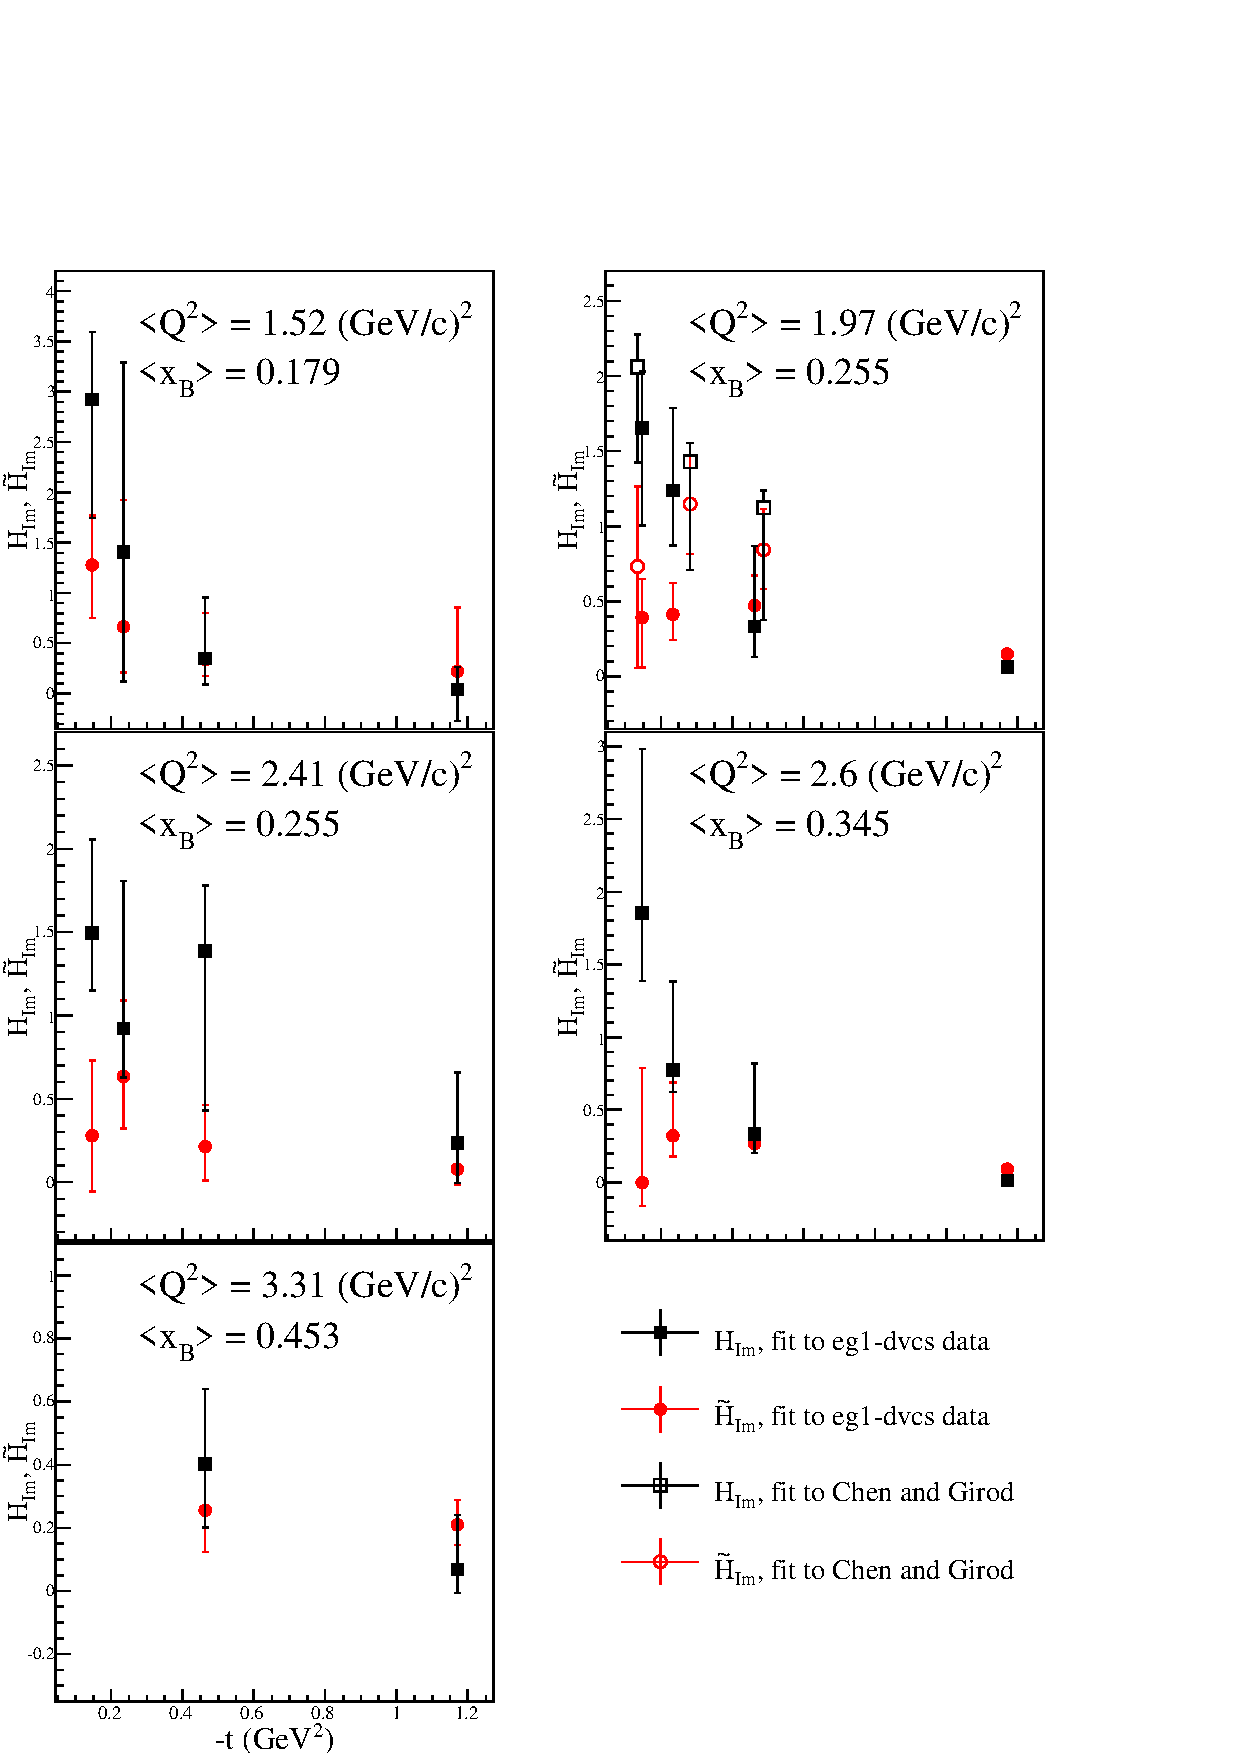
\includegraphics[width=120mm]{CFF_comp_prop.pdf}
\caption[$t$ dependence of $H_{lm}$ and $\tilde{H}_{lm}$.]
{$t$ dependence for each $Q^2$-$x_B$ bin of $H_{Im}$ (black squares) and $\tilde{H}_{Im}$ (red circles). The full points are obtained by fitting the eg1-DVCS data (TSA, BSA and DSA) \cite{pisano}. The empty points were obtained by fitting the BSA results from \cite{fx} integrated over all values of $Q^2$ at $x_B \sim 0.25$, and the TSAs from \cite{shifeng}.}
\label{cffs_eg1dvcs}
\end{center}
\end{figure}

%\input{Exp_situation}
%\input{Setup}
%\input{Poltar}
%\subsection{Central Neutron Detector}\label{cnd-section}
The Central Neutron Detector was conceived to extend the CLAS12 acceptance for the recoil neutrons of nDVCS, which are expected to be mostly emitted between $50^{\circ}$ and $70^{\circ}$ \cite{proposal}. The requirements of the detector are:
\begin{itemize}
\item{good capabilities for neutron identification, via the measurement of $\beta$ (with $\beta=\frac{v}{c}$), for the kinematic range of interest ($0.2<p_n<1.2$ GeV/c, $40^o<\theta_n<80^o$)} and
\item{neutron momentum resolution $\sigma_P/P$ within 10\%,}
\end{itemize}
Early simulation studies \cite{proposal} showed that these performances can be achieved by a scintillator-based detector providing a timing resolution of about 150 ps. 

\begin{figure}[ht]
\begin{center}
\includegraphics[width=3.5in]{CND_bello.pdf}
\end{center}
\caption [Design of the Central Neutron Detector]
{Design of the Central Neutron Detector, inserted in the CLAS12 solenoid.}
\label{cnd_nice}
\end{figure}

The core of the CND (Fig.~\ref{cnd_nice}), which will be placed in the Central Detector, in the 10 cm of radial space left between the Central Time Of Flight (CTOF) and the solenoid magnet, is a barrel, coaxial with the beam direction, made of three radial layers of trapezoidal plastic-scintillator bars. 
Each radial layer contains 48 bars, connected in pairs by a "u-turn" light guide at the downstream end.
Photomultipliers are coupled to the upstream end of each scintillator via 1.5m-long light guides. For each hit, half of the light emitted in a scintillator paddle is collected by the upstream PMT (the ``direct'' signal), while the other half propagates through the u-turn and the neighboring paddle to the PMT connected at its end (the ``indirect'' signal). 

Three such scintillator pairs (inner, middle, and outer) are grouped together to form a single, radial "block".  The CND comprises 24 of these blocks, covering the entire azimuthal range (Fig.~\ref{CND_Orsay}).

\begin{figure}
\begin{center}
    \includegraphics[height=40mm]{block_tested_2.pdf}
    \includegraphics[height=40mm]{cnd_finito.jpg}
  \caption{Construction and testing of the CND at Orsay. Left: one 2x3 block undergoing cosmic ray tests.  Right: all 24 blocks installed into a mock-up of the CLAS12 solenoid.}
  \label{CND_Orsay}
\end{center}
\end{figure}
The assembly of the CND, which was entirely carried out at the IPN Orsay, started in December 2013, and was completed in February 2015. The detector was shipped and stored at JLab in June 2015, awating its installation in CLAS12. Upon assembly, each block of the CND was tested with cosmic rays, triggering on the triple-coincidence of the signal in all three layers. Data were taken for about one week for each block, and the block performances were studied, with special attention to the timing resolution. 
Figure~\ref{tdc_adc_raw} shows the raw distribution of TDCs as a function of ADCs for the six PMTs in one of the 24 blocks. Notice the clear separation between direct (low-TDC/high-ADC) and indirect (high-TDC/low-ADC) signals. 

To define an average time resolution for our setup in the triple-coincidence trigger configuration, we use the method inspired by the work done in \cite{giles} and later adopted for the CLAS TOF system \cite{elton_paper}. 

\begin{figure}
\begin{center}
\includegraphics[width=140mm]{tdc_adc_raw.pdf}
\caption[Cosmic ray data for the CND]
{Cosmic rays data. Raw TDC vs ADC for each of the six PMTs of block 2 of the CND. No pedestal subtraction or data-cleaning cuts are applied.}
\label{tdc_adc_raw}
\end{center}
\end{figure}

\begin{figure}
\begin{center}
\includegraphics[width=80mm]{res_blocks.pdf}
\caption[Time resolution of the CND]
{Average time resolution for each block of the CND from cosmic rays measurements in triple-coincidence. The black and red triangles are the results obtained with the formulae from, respectively, Refs.~\cite{elton_paper} and \cite{vitali}.}
\label{res_blocks}
\end{center}
\end{figure}

The timing resolutions for all the CND blocks, computed according to the method of \cite{elton_paper}, are represented by the black triangles in Fig.~\ref{res_blocks}. The average is 148.0 ps. As a cross check, the resolution was also computed using the method adopted by V. Baturin for the CLAS12 CTOF \cite{vitali} (red triangles in Fig.~\ref{res_blocks}, with average 149.3 ps). The results of the two methods are consistent. The resolutions of the 24 blocks are very close to the required 150 ps. The systematic uncertainty of our results is estimated to be about $7\%$, determined by repeating the measurements multiple times, and by comparing multiple subsets of each measurement. 

Thus, for resolutions of 150 ps, we have a systematic uncertainty of about 10 ps.

It is also worth mentioning that the TDCs that will be used for the actual experiment will have a better resolution (25ps/channel) than the ones used for these tests (50ps/channel).

\subsection{Simulation and reconstruction}\label{sim_sec}
\begin{figure}[htb]
\begin{center}
\includegraphics[width=80mm]{CND_4.pdf}
%\vspace{-3.5cm}
\caption {Geometry of the Central Neutron Detector in the GEMC simulation, showing three layers of scintillator paddles (green) coupled in pairs via u-turn light guides (blue) downstream.}
\label{cnd_gemc}
\end{center}
\end{figure}

In order to study the performances of this detector, and thus evaluate the projected results of the nDVCS experiment, its geometry (Fig.~\ref{cnd_gemc}) has been added to the CLAS12 GEANT4-based simulation package, GEMC \cite{mauri}. The energy loss of the particle in the scintillator material is converted to numbers of optical photons in accordance with Birk's formula \cite{birks}, the resulting signal is propagated through the scintillator paddle, light guide and PMT, and the final charge and time are digitized to mimic the output from the ADC/TDC \cite{daria_wiki}.

The timing resolution and the energy loss due to the u-turn geometry have been included in the simulation using the values measured in the cosmic-rays tests described in the previous section. 

Simulations, which included all the other components of the Central Detector, have been run to evaluate the efficiency of the CND for neutrons, its ability to discriminate between neutrons and photons, and its angular and momentum resolutions. Neutrons and photons of momenta varying between 0.1 and 1 GeV/c and having polar angles $\theta$ varying between $50^o$ and $70^o$ have been generated at fixed azimuthal angle ($\phi = 0^o$), pointing to the center of one of the scintillator bars. The results obtained with these simulations are described here below..

\subsubsection{Efficiency}\label{efficiency-section}

 The detection efficiency is defined here as the ratio between the number of events for which a good hit (i.e., a hit having deposited energy above a given threshold) was successfully reconstructed as a neutron in the correct azimuthal bin of the CND and the total number of neutrons generated. 
Several values of energy thresholds, between 1 and 5 MeV, have been tested. 
The efficiency decreases with increasing threshold, and ranges between 12\% at the lowest thresholds and 7\% at the highest ones. 
Figure~\ref{eff_vs_mom} shows the efficiency as a function of the momentum of the neutrons, at a fixed energy threshold of 2 MeV, and for different values of $\theta_n$. 

\begin{figure}[t]  
\begin{center}
\includegraphics[width=100mm]{eff_vs_mom_diff_theta_II.pdf}
\caption [Neutron detection efficiency as a function of neutron momentum]
{Efficiency for the detection of neutrons, as a function of neutron momentum, for a 2-MeV threshold on the deposited energy. The efficiency is shown for three different values of $\theta_n$, between $50^o$ and $70^o$.
}
\label{eff_vs_mom}
\end{center}
\end{figure}

\subsubsection{Angular and momentum resolutions}\label{resolution-section}

The resolutions on the polar angle $\theta$ of the neutron that can be obtained with the CND are strongly linked to its TOF resolution. The angle $\theta$ is in fact given by
\begin{eqnarray} 
\theta = (180/\pi)\cdot \arccos (\frac{z_{ave}}{l})
\end{eqnarray}
where the reconstructions of the radial distance of the hit from the target, $l$, and of its position along the scintillator bar, $z_{ave}$,  both depend on the time measurement. Using a value deduced from the measurements on the CND prototype to apply a gaussian smearing on the timing \cite{proposal}, 
%\begin{equation}\label{eq_time_smear}
%\sigma_t=\frac{A}{\sqrt{E_{dep}}}, 
%\end{equation}
%(see Appendix~\ref{sec_rec})
the $\theta$ resolution resulting from GEMC was studied as a function of neutron momentum and $\theta$ itself. The results are shown in Fig.~\ref{theta_n_tofcut5}, where the angular resolution $\sigma_\theta$, obtained via gaussian fits of the simulated $\theta$ distributions, is plotted as a function of  $\theta$, for a particular value of neutron momentum (0.4 GeV/c). $\sigma_\theta$ is seen to increase slightly with the angle, from $1.5^{\circ}$ to $3.5^{\circ}$.  It has also been found to be relatively insensitive to the neutron momentum. 

The resolution on the azimuthal angle is directly connected to the total number of scintillator bars along $\phi$. In fact, the bin size $\Delta\phi$ is given by
\begin{eqnarray} 
\Delta\phi = \frac{360^{\circ}}{N}=7.5^{\circ}
\end{eqnarray}
where $N$ is the total number of paddles in $\phi$ (48 for the final design of the CND). $\sigma_\phi$ can be taken as half of $\Delta\phi$, therefore $3.75^o$.
\begin{figure}[hbt]  
\begin{center}
\includegraphics[width=100mm]{sigma_theta_vs_theta_diff_layer.pdf}
\caption [Angular resolution of the CND as a function of $\theta$]
{Angular resolution $\sigma_\theta$ as a function of $\theta$ for neutrons of momentum 0.4 GeV/c, for a 2-MeV threshold on the deposited energy. The three colors of the points correspond to the three radial layers of the CND.}
\label{theta_n_tofcut5}
\end{center}
\end{figure}

\begin{figure}  
\begin{center}
\includegraphics[width=100mm]{mom_res_vs_mom_diff_layers.pdf}
\caption [Momentum resolution as a function of $p$]
{Momentum resolution $\sigma_p/p$ as a function of $p$ for neutrons having $\theta=60^o$, for a 2-MeV threshold on the deposited energy. The three colors of the points correspond to the three radial layers of the CND.}
\label{p_n_tofcut5}
\end{center}
\end{figure}

The resolution on the neutron momentum, calculated after particle identification on the basis of $\beta$, according to the formula
\begin{eqnarray}
p = \frac{\beta\cdot m_n}{\sqrt{1-\beta^2}},
\end{eqnarray}
is also strictly connected to the TOF resolution. Figure \ref{p_n_tofcut5} shows the momentum resolution $\sigma_p/p$ as a function of momentum for neutrons emitted with $\theta=60^o$: it increases with increasing momentum, and ranges between 4\% and 11\%. No appreciable variations of momentum resolution are observed by varying the neutron polar angle.


\subsubsection{Particle Identification}\label{pid-section}

Since the charged particles passing through the CND will be vetoed by the Central Tracker, the only particles that could be mistaken for neutrons in the CND are the photons. 
The efficiency of the CND for detecting photons (Fig.~\ref{eff_photons}) has been estimated in simulations to be similar to that for neutrons, about 10\% for photon energies down to 0.2 GeV.  The efficiency drops to zero for lower energy photons, depending on the threshold cut applied. 

\begin{figure}  
\begin{center}
\includegraphics[width=100mm]{efficiency_photons_60deg_new.pdf}
\caption [Photon detection efficiency as a function of photon momentum]
{Efficiency for the detection of photons, as a function of photon momentum, for a 2-MeV threshold on the deposited energy. The efficiency is shown for $\theta_{\gamma}=60^o$. Below $E_\gamma=0.15$ GeV, the photon efficiency drops to zero.}
\label{eff_photons}
\end{center}
\end{figure}

\begin{figure}
\begin{center}
\includegraphics[width=80mm]{beta_comp_layer_2_II.pdf}
\caption [$\beta$ distributions for neutrons and photons in the CND]
{$\beta$ distributions for neutrons with $p_n=0.2$ GeV/c (green), $p_n=0.4$ GeV/c (purple), $p_n=0.7$ GeV/c (blue), $p_n=1$ GeV/c (red), and photons with $E=1$ GeV, for the middle layer of the CND. 
The threshold on the deposited energy is 2 MeV. The plots show all hits, integrated over $\phi$. Equal neutron and photon yields have been assumed here.}
\label{beta_n_g}
\end{center}
\end{figure}

\begin{figure}
\begin{center}
\includegraphics[width=100mm]{beta_res_n_g_comp_L2.pdf}
\caption [$\beta$ versus momentum for neutrons and photons in the CND]
{$\beta$ versus momentum for neutrons (red) and photons (blue) with momenta between 0.2 and 1 GeV, for the middle layer of the CND. The error bars are defined as $3\sigma$, where $\sigma$ is the fitted width of each $\beta$ peak. The threshold on the deposited energy is 2 MeV.}
\label{fig_beta_res}
\end{center}
\end{figure}

Neutrons can be discriminated from photons by means of their $\beta$, and so GEMC simulations have been performed to estimate the $\beta$ distributions that may be obtained from the CND.  Results for one of the three radial layers, integrated over the azimuthal angle, is shown in Figure~\ref{beta_n_g}.  Here $\beta$ distributions for neutrons with momenta between 0.2 and 1 GeV/c are compared with 1 GeV photons.  Very clear separation is evident for neutrons less than about 0.9 GeV/c, which comprise over 90\% of the expected nDVCS events. 

This is evident also from Fig.~\ref{fig_beta_res}, where the error bars correspond to $3 \sigma$, where $\sigma$ is the gaussian width of each $\beta$ distribution. Equal neutrons and photon yields have been assumed for this study. This assumption has been justified with detailed studies on the different types of photonic backgrounds that can affect the CND \cite{proposal}.

%\input{Analysis}
%\section{Projected results}\label{sec_countrate}
A GPD-based event generator for DVCS-BH on a deuterium target was run, assuming a luminosity of $3/20\cdot 10^{35}$ cm$^2$ s$^{-1}$ (where the factor $3/20$ accounts for the ratio of polarized neutrons to the total nucleons in ND$_3$) and a beam time of 100 days. The output of the generator was fed to the CLAS12 Fast-MC code, which included acceptance and resolution effects for CLAS12 and the CND. An additional factor of $10\%$ was also applied to mimick the efficiency of the CND for neutrons\footnote{Actually, this factor was adopted globally for ALL neutrons, even those falling within the EC acceptance. Given that the EC should have higher neutron efficiency than the CND, by at least a factor of 2, the projections for the count rates shown here are slightly pessimistic.}. nDVCS exclusivity cuts were then applied. This way, the expected yields for the $en\gamma(p)$ events produced on the ND$_3$ target were obtained. The kinematic space (in $Q^2$, $x_B$, $-t$, $\phi$) available with the acceptance of the CLAS12+CND setup was divided into the same 4-dimensional grid that was used for the unpolarized nDVCS proposal:
\begin{itemize}
\item{4 bins in $Q^2$, the limits of which are: 1, 2, 3.5, 5, 10 (GeV)$^2$;}
\item{4 bins in $x_B$, the limits of which are: 0.05, 0.15, 0.3, 0.45, 0.7;}
\item{4 bins in $-t$, the limits of which are: 0, 0.2, 0.5, 0.8, 1.2 (GeV)$^2$;}
\item{12 bins in $\phi$.}
\end{itemize}

The central kinematics for each bin were computed as weighted averages over the reconstructed events. The target-spin asymmetry and the double-spin asymmetry were then calculated as a function of $\phi$ using the VGG model (with input parameters $J_u=0.3$ and $J_d=0.1$) for each of the ($Q^2$, $x_B$, $-t$) bins that are kinematically allowed. 
Statistical errors were then obtained for these asymmetries using the approximated formula: 
\begin{equation}\label{error_asym}
\sigma_A = \frac{1}{P}\cdot \frac{\sqrt{1-P^2\cdot A^2}}{\sqrt{N}}.
\end{equation}
where $P$ is the polarization (and it is therefore equal to the target polarization for neutrons, $P_t$, for the TSA case, and to the product of beam and target polarizations, $P_bP_t$, for the DSA case), and $N$ is the expected yield in each 4-dimensional bin. % (Figs.~\ref{count_rate_1} and \ref{count_rate_2}). 

The resulting asymmetries with the associated expected error bars are shown in Figs.~\ref{fig_tsa_100_50_FT} (TSA) and \ref{fig_dsa_100_50_FT} (DSA). These same figures also show the comparison, for TSA and DSA, for running this experiment with either 50 or the proposed 110 days of beam time. 
The use of the Forward Tagger will improve the $\phi$ coverage at the edges ($\phi\to 0^{\circ}$ and $\phi\to 360^{\circ}$) for some of the low-$t$ bins, which is otherwise incomplete. This can be noticed in Figs.~\ref{fig_tsa_100_50_FT} and \ref{fig_dsa_100_50_FT}, where at the edges of several of the $\phi$ distributions only the black points are present. 

%For reference, the 4-dimensional acceptances obtained with the simulation are shown in Figs.~\ref{acceptance_1} and \ref{acceptance_2}. 

It is important to point out that the number of days chosen here (110) is the minimal amount of time necessary to be able to bin the TSA and the DSA in enough kinematic bins to describe in a satisfactory manner the dependence in all the 4 kinematic variables, while at the same time having statistical uncertainties not exceeding too much the ones expected for the BSA of E12-11-003 (Fig.~\ref{fig_bsa}). 

%\begin{sidewaysfigure}  
%\begin{center}
%\includegraphics[width=200mm]{asym_polndvcs_tsa_newvgg_100days_FT_noFT.pdf}
%\caption[Projected target-spin asymetry]
%{Projected target-spin asymmetry. The y-scale range, common to all bins, is (-1;1). The black and red points are obtained, respectively, without and with the Forward Tagger. }\label{fig_tsa}
%\end{center}
%\end{sidewaysfigure}

\begin{sidewaysfigure}  
\begin{center}
\includegraphics[width=200mm]{asym_polndvcs_tsa_newvgg_100_FT_and_noFT_50days.pdf}
\caption[Projected target-spin asymetry]
{Projected target-spin asymmetry. The y-scale range, common to all bins, is (-1;1). The black and red points are obtained, respectively, with 110 days and 50 days of beamtime.}\label{fig_tsa_100_50_FT}
\end{center}
\end{sidewaysfigure}

\begin{sidewaysfigure}  
\begin{center}
\includegraphics[width=200mm]{asym_polndvcs_dsa_newvgg_BH_100_50days_FT_and_noFT.pdf}
\caption[Projected double-spin asymmetry]
{Projected double-spin asymmetry, compared to the BH (green lines), calculated at the average kinematics of each bin. The y-scale range, common to all bins, is -0.6-1.2. The black and red points are obtained, respectively, with 110 days and 50 days of beamtime. }\label{fig_dsa_100_50_FT}
\end{center}
\end{sidewaysfigure}

\begin{sidewaysfigure}  
\begin{center}
\includegraphics[width=160mm]{asym_newcuts_bsa_newvgg.pdf}
\caption[Projected beam-spin asymmetry from E12-11-003]
{Projected beam-spin asymmetry, as will be obtained from experiment E12-11-003 \cite{proposal}. The y-scale range, common to all bins, is -0.25-0.25.}\label{fig_bsa}
\end{center}
\end{sidewaysfigure}

%\input{CFF_Results}
%\section{Systematic uncertainties}\label{sec_syst}
The goal of this experiment is to extract target and double-spin asymmetries, which are ratios of polarized cross sections. In the ratio, polarization-independent terms, such as acceptances, efficiencies, radiative corrections and luminosity, cancel out to a first approximation\footnote{Afanasev {\it et al.} \cite{afanasev} have computed the radiative corrections for the DVCS and BH processes on for CLAS kinematics. It was found that, given the strict kinematic cuts adopted to select the final state, the undetected radiated photon can only have small energies. In this case, therefore, the main contribution to the radiative correction comes from spin-independent soft-photon emission that does not affect the polarization observables. The approximation of negligible contribution from the radiative corrections to the BSA, TSA and DSA, compared to the size of the asymmetries, was estimated to be valid at the 0.1\% level \cite{afanasev}.}. Remaining effects could come from the quantities entering in the asymmetry definitions, namely the procedure to evaluate the counts $N^{+(-)}$, the dilution factor, the $\pi^0$ contamination, as well as the beam and target polarizations. 

Analyses performed at 6 GeV \cite{erin,pisano} showed that the biggest contributor to the overall systematic uncertainty is the selection of exclusivity cuts adopted to identify DVCS events and the corresponding counts $N^{+(-)}$. This factor contributed about 10\% (this and the following percentages for systematics are defined relatively to the average value of the TSA at $90^{\circ}$) to the total systematics uncertainty. 

Another source of uncertainty will be the $\pi^0$ background estimation, which will depend on the accuracy of the description of the detector acceptance and efficiency and on the model used in the Monte-Carlo simulation to describe the $en\pi^0(p)$ reaction (see Eq. 32). In order to account for this latter effect, 6-GeV analyses, performed on data taken on a polarized NH$_3$ target during the eg1-dvcs experiment \cite{erin,pisano}, evaluted this systematic by varying the contribution of the calculated background by $\pm 30\%$ (Section \ref{sec_pi0_back}), and extracting the final asymmetries in correspondence with this increased/decreased background. The total effect turned out to be 4\%, and a similar estimation can be assumed for the present experiment on ND$_3$.

While acceptance effects are expected to cancel in asymmetries, a residual effect could emerge due to the strong variations of the cross section inside the finite-size bins, that can lead, in principle, to a non-exact cancellation of acceptance effects from the numerator and the denominator. Such an acceptance effect has been estimated to bring an additional 1\% systematic error. 

To evaluate the systematic uncertainties linked to the dilution factor determination, in the aforementioned eg1-dvcs pDVCS analysis the  asymmetries were computed two more times, taking two different values of the dilution factor: $D_f+\Delta(D_f)$ and $D_f-\Delta(D_f)$, where $\Delta(D_f)$ is the statistical error that was estimated on this quantity. The resulting systematic uncertainties were found to be below the percent level. While studying the systematics on the exclusivity cuts, it was observed that changing the exclusivity cuts induces a variation of the dilution factors much bigger than the variations within the statistical errors described above. It was therefore decided, in order to avoid double-counting and therefore overestimation of systematics, to remove the contribution from the dilution factor computed according to its errors from the total systematic uncertainty. For this proposal, instead, a conservative estimate of the systematic uncertainty on the dilution factor of the order of 3\%, consistent with previous assumptions \cite{kuhn}, is assumed. 

%As for the systematic uncertainties on the dilution factors, in the aforementioned pDVCS 6-GeV analysis of eg1-dvcs were included in the exclusivity cut ones. Indeed, the systematic effect due to the variation of the exclusivity cuts represents the biggest contribution to the overall systematics, and, being the dilution factor strictly related to the specific set of exclusivity cuts adopted, its variation between the different sets of cuts turned out to be larger than its statistical error, making unnecessary a dedicated study.

An additional 2\% systematic effect is included in the total budget to account for the possible misidentification of neutrons due to accidental coincidences (Section~\ref{sec_accidentals}.)

Finally, uncertainties in the knowledge of the beam and target polarizations (extracted, respectively, via M{\o}ller polarimetry measurements and via the NMR system) will propagate into the asymmetry measurements, and are expected to lead to contributions of, respectively, 3\% and 4\%.

A summary of the systematic uncertainties can be found in Table~\ref{table_syst}. The total systematic uncertainty will be of the order of 12\%, averaged over all the kinematic bins (the $\pi^0$-background uncertainty will actually vary depending on the bin). 

\begin{table}
\begin{center}
\begin{tabular}{|c||c|}
\hline
Source of error & Systematic uncertainty\\
\hline
Channel selection cuts & 10\% \\
\hline
Beam and target polarization & 3\%-4\%  \\
\hline
$\pi^0$ contamination & 4\%  \\
\hline
Acceptance & 1\%  \\
\hline
Dilution factor & 3\%  \\
\hline
Accidentals & 2\%  \\
\hline
Radiative corrections & Negligible  \\
\hline
\hline
Total & 12\%  \\
\hline
\end{tabular}
\caption{Expected systematic uncertainties on the proposed measurement.}
\label{table_syst}
\end{center}
\end{table}

%\input{Request}


\newpage
\begin{thebibliography}{999}
\bibitem{muller}
D. M\"uller, D. Robaschik, B. Geyer, F.-M. Dittes, and J. Horejsi, Fortschr. Phys. {\bf 42} (1994) 101.
\bibitem{ji} X. Ji, Phys. Rev. Lett. {\bf 78} (1997) 610;
Phys. Rev. D {\bf 55} (1997) 7114.
\bibitem{rady} A.V. Radyushkin, Phys. Lett. B {\bf 380} (1996) 417; Phys. Rev. D {\bf 56} (1997) 5524.
\bibitem{collins} J.C. Collins, L. Frankfurt and M. Strikman, Phys. Rev. D {\bf 56} (1997) 2982.
\bibitem{goeke} K. Goeke, M. V. Polyakov and M. Vanderhaeghen, Prog.\ Part.\ Nucl.\ Phys. {\bf 47} (2001) 401.
\bibitem{revdiehl} M. Diehl, Phys.  Rept. {\bf 388} (2003) 41.
\bibitem{revrady} A.V. Belitsky, A.V. Radyushkin, Phys. Rept. {\bf 418} (2005) 1.
\bibitem{proposal} S. Niccolai, V. Kubarovsky, S. Pisano, and D. Sokhan, JLab experiment E12-11-003.
\bibitem{belitski} A.V. Belitsky, D. M\"uller, A. Kirchner, Nucl. Phys. B {\bf 629} (2002) 323-392.
\bibitem{fitmick} M. Guidal, Eur. Phys. J. A {\bf 37} (2008) 319; M. Guidal, H. Moutarde, Eur. Phys. J. A 42 (2009) 71.
\bibitem{mick_herve} M. Guidal, H. Moutarde, M. Vanderhaeghen, Rep. Prog. Phys. {\bf 76}, 066202 (2013).
\bibitem{vgg} M. Vanderhaeghen, P.A.M. Guichon, M. Guidal, Phys. Rev. D {\bf 60}, 094017 (1999).
\bibitem{vgg1} M. Guidal, M. V. Polyakov, A. V. Radyushkin and 
M. Vanderhaeghen, Phys.\ Rev. D {\bf 72}, 054013 (2005).
\bibitem{pisano} S. Pisano {\it et al.}, Phys. Rev. {\bf D91}, 052014 (2015).
\bibitem{erin} E. Seder {\it et al.}, Phys. Rev. Lett. {\bf 114}, 032001 (2015).
\bibitem{fx} F.-X. Girod {\it et al.}, Phys. Rev. Lett. {\bf 100}, 162002 (2008).
\bibitem{shifeng} S. Chen {\it et al.}, Phys. Rev. Lett. {\bf 97}, 072002 (2006).
\bibitem{malek} M. Mazouz et al., Phys.\ Rev.\ Lett. {\bf 99}, 242501 (2007).
\bibitem{carlos} C. Mu\~noz Camacho {\it et al.} (Hall-A Collaboration), Phys. Rev. Lett. {\bf 97}, 262002 (2006).
\bibitem{stepan} S. Stepanyan {\it et al.} (CLAS Collaboration), Phys. Rev. Lett. {\bf 87}, 182002 (2001).
\bibitem{hermes} A. Airapetian {\it et al.} (HERMES Collaboration), JHEP06 {\bf 0806}, 066 (2008); A. Airapetian {\it et al.} (HERMES Collaboration), JHEP {\bf 06}, 019 (2010).
\bibitem{hs} H.-S. Jo {\it et al.}, arXiv:1504.02009 [hep-ex].
\bibitem{E1206114}  C. Hyde-Wright, B. Michel, C. Munoz Camacho and J. Roche, JLab experiment E12-06-114.
\bibitem{E1206119} F. Sabati\'e, A. Biselli, V. Burkert, L. Elouadrhiri, M. Gar\c{c}on, M. Holtrop, D. Ireland, K. Joo, W. Kim, JLab experiment E12-06-119.
\bibitem{E1212010}  L. Elouadrhiri, H. Avakian, V. Burkert, M. Guidal, M. Lowry, L. Pappalardo, and S. Procureur, JLab experiment E-12-12-010, conditionally approved.
\bibitem{E07007} C. Munoz Camacho, C. Hyde-Wright, P.-Y. Bertin, JLab experiment E07-007.
\bibitem{E1213010} C. Munoz Camacho, R. Paremuzyan, T. Horn, JLab experiment E12-13-010. 
\bibitem{E08025} C.H. Hyde, P.-Y. Bertin, A. Camsonne, JLab Experiment E08-025.
\bibitem{batta} Technical Design Report of the CLAS12 Forward Tagger, {\rm http://www.ge.infn.it/\textasciitilde batta/jlab/ft-tdr.2.0.pdf}.
\bibitem{Goertz2002} St. Goertz, W. Meyer, and G. Reichertz, Progress in Particle and Nuclear Physics {\bf 49} (2002) 403.
\bibitem{Court1993} G.R. Court, D.W. Gifford, P. Harrison, W.G. Heyes, and M.A. Houlden, Nucl. Instr. Meth. {\bf A 324}, 433 (1993). 
\bibitem{Court2004} G.R. Court, {\it et al.}, Nucl. Instr. Meth. {\bf A 527}, 253 (2004).
\bibitem{Dulya1997}  C. Dulya, {\it et al}, Nucl. Instr. and Meth. A \textbf{398} (1997) 109.
\bibitem{Kwaltine2013} N. D. Kwaltine, PhD thesis, University of Virginia, 2013.
\bibitem{Slifer2007} K. Slifer, ``Proceedings of the 12th International Workshop on Polarized Ion Sources, Targets, and Polarimetry'', Upton, NY (2007) 330.
\bibitem{McKee2004} P. McKee, Nucl. Instr. Meth. {\bf A 526}, 60 (2004).
\bibitem{giles} R.T. Giles {\it et al.}, Nucl. Instr. Meth. {\bf A 252}, 41 (1986).
\bibitem{elton_paper} E. Smith {\it et al.}, Nucl. Instr. Meth. {\bf A 432}, 265 (1999).
\bibitem{vitali} V. Baturin {\it et al.}, Nucl. Instr. Meth. {\bf A 562}, 327 (2006).
\bibitem{mauri} M. Ungaro, private communication.
\bibitem{birks} J.B. Birks, Proc. Phys. Soc. {\bf A64}, 874 (1951).
\bibitem{daria_wiki} D. Sokhan, http://clasweb.jlab.org/wiki/index.php/Daria .
\bibitem{silvia_wiki} S. Niccolai, {\rm http://clasweb.jlab.org/rungroups/e1-dvcs/wiki/index.php/CLAS12 neutron detector:update on simulation (September 2008)}.
\bibitem{ahmed} A. El Aloui and E. Voutier, CLAS-NOTE 2009-024.
\bibitem{harut} H. Avakyan, private communication.
\bibitem{paris} M. Lacombe et al., Phys. Rev C {\bf 21} (1980) 861.
\bibitem{daria_eg1dvcs} D. Sokhan, analysis underway. 
\bibitem{peter_exclusive} P. Bosted {\rm https://www.jlab.org/Hall-B/secure/eg1-dvcs/bosted/Exclusive/exclnote.pdf}.
\bibitem{raffa}  R. De Vita, private communication.
\bibitem{sidis_prop} A. Avakian {\it et al.}, JLab conditionally approved proposal C12-11-111. 
\bibitem{procureur} S. Procureur, private communication.  
\bibitem{afanasev} A.V. Afanasev {\it et al.}, J. Exp. Theor. Phys. {\bf 102}, 220 (2006).
\bibitem{kuhn} S. Kuhn, A. Deur, V. Dharmawardane, K. Griffioen, D. Crabb, Y. Prok, T. Forest, Jefferson Lab Experiment E12-06-109.
\bibitem{schedule} {\rm https://www.jlab.org/Hall-B/clas12-web/clas12-expt1.jpg}.

\end{thebibliography}


%\appendix
\section{Appendix: Count rates and acceptances for the "FT" and "no-FT" configurations}
\begin{figure}  
\begin{center}
\includegraphics[width=130mm]{plot_counts_1_FT_noFT_100days.pdf}
\includegraphics[width=130mm]{plot_counts_2_FT_noFT_100days.pdf}
\caption{Expected count rates for the nDVCS channel: $0.<-t<0.2$ GeV$^2$ (top) and $0.2<-t.0.5$ GeV$^2$ (bottom). Black: with FT; red: without FT. \label{count_rate_1}
}
\end{center}
\end{figure}
\begin{figure}  
\begin{center}
\includegraphics[width=120mm]{plot_counts_3_FT_noFT_100days.pdf}
\includegraphics[width=120mm]{plot_counts_4_FT_noFT_100days.pdf}
\caption{Expected count rates for the nDVCS channel: $0.5<-t<0.8$ GeV$^2$ (top) and $0.8<-t<1.2$ GeV$^2$ (bottom). Black: with FT; red: without FT.\label{count_rate_2}}
\end{center}
\end{figure}

\begin{figure}  
\begin{center}
\includegraphics[width=130mm]{plot_acc_1_FT_noFT_100days.pdf}
\includegraphics[width=130mm]{plot_acc_2_FT_noFT_100days.pdf}
\caption{Expected acceptances, including the 10\% of efficiency for the CND, for the nDVCS channel: $0.<-t<0.2$ GeV$^2$ (top) and $0.2<-t<0.5$ GeV$^2$ (bottom). All plots have $y$ scale ranging from 0 to 0.05 Black: with FT; red: without FT.. \label{acceptance_1}}
\end{center}
\end{figure}
\begin{figure}  
\begin{center}
\includegraphics[width=120mm]{plot_acc_3_FT_noFT_100days.pdf}
\includegraphics[width=120mm]{plot_acc_4_FT_noFT_100days.pdf}
\caption{Expected acceptances, including the 10\% of efficiency for the CND, for the nDVCS channel: $0.5<-t<0.8$ GeV$^2$ (top) and $0.8<-t<1.2$ GeV$^2$ (bottom). All plots have $y$ scale ranging from 0 to 0.05. Black: with FT; red: without FT. \label{acceptance_2}}
\end{center}
\end{figure}


\end{document}

\newpage
\chapter{Additional physics topics}
\abstract{Ideas for additional physics topics that the extension to 110 days of running time on polarized ND$_3$ will allow to study are presented here. An increased statistics on ND$_3$ will permit to measure, for the first time, the semi-inclusive production of hadron pairs on longitudinally polarized deuterium. This can provide a unique access to the poorly known chiral-odd PDFs, which can then be separated according to their flavor via the combination with the results obtained on proton and deuteron targets. 
Likewise, these data would permit a first-time measurement of single and double target spin asymmetries for time-like Compton scattering on the neutron, which provides an alternative way to DVCS for the measurement of GPDs. 
Finally, measurements of meson electroproduction on the longitudinally polarized neutron could serve to address specific questions relative to the quantum numbers of the $t$-channel exchanges mediating meson production, or to the GPDs, in the hard regime.}
\newpage
\setcounter{page}{96}
\section{Semi-inclusive production of hadron pairs}
In addition to the semi-inclusive production of single hadrons, other semi-inclusive channels would benefit from an increased statistics on a longitudinally polarized deuteron target. 
In the last years, for example, an increasing role is being played by the SIDIS production of hadron pairs, which gives the cleanest access to the chiral-odd one-dimensional picture of the nucleon. Differently from the quark (unpolarized) and helicity 1D distribution functions, the transversity distribution, as well as the two higher-twist PDF $e(x)$ and $h_L(x)$, cannot be accessed through inclusive DIS. This is due to their chiral-odd nature, that prevents the access through inclusive observables. In order to be accessed, indeed, they have to appear in the observables coupled to a second chiral-odd function, the so-called Di-Hadron fragmentation functions. The latter are the analogous of the single hadron FFs described earlier in the text, and encode the fragmentation of the struck quark to the final hadron pair. 
The main advantage of the di-hadron production is the fact that, while in the single-hadron case the distribution functions and the fragmentation functions appear coupled in the structure functions through a convolution integral, in the di-hadron case they are coupled through a simple product, making the final extraction easier and less sensitive to model assumptions. 
Among the chiral-odd PDFs, the higher-twist $H_1(x)^\sphericalangle$ is by far the least known. It can only be accessed through the di-hadron longitudinal target-spin asymmetry, where it appears coupled to the interference fragmentation functions $h_{1L}^\sphericalangle$, that represents the analogous of the Collins function of the single-hadron case. 
Together with $e(x)$, it opens the avenue to a deeper understanding of the quark-gluon-quark correlations inside the nucleon. No measurements of such an observable are presently available on a deuteron target. Preliminary analysis on a $NH_3$ target by CLAS shows a first non zero $A_{UL}$ on the proton. This preliminary observation would be greatly improved by a high-precision extraction in the extended kinematics accessible by CLAS12, both on a proton and on a deuteron target. A combined measurement of the di-hadron $A_{UL}$ on both proton and deuteron will be highly beneficial, since it will allow to perform the flavor separation of the PDFs and of the di-hadron FF. As for the single-hadron case, in order to properly disentangle the dependencies of the PDFs and the FFs, a multidimensional mapping will be essential. Due to the reduced phase-space for the di-hadron case with respect to single hadron, high statistics will be essential to reach a proper accuracy in all the bins. 

\section{Time-like Compton Scattering on longitudinally polarized deuteron}
Time-like Compton scattering (TCS), the photoproduction of a virtual photon on the nucleon at the quark level, is an alternative way to DVCS to gain access to the Generalized Parton Distribution. 
The $\gamma N \to Ne^+e^-$ reaction consists of two processes: the Bethe-Heitler (Fig.~\ref{tcs_diagram}, bottom), a pure QED process in which the final-state lepton pair originates directly from the initial photon of the beam, and the TCS (Fig.~\ref{tcs_diagram}, top). 
\begin{figure}[htbp] 
   \centering
   \includegraphics[width=6in]{TCS_handbag_bold_bis.png} 
   \includegraphics[width=4in]{BH_diag_TCS.png} 
   \caption{Top: the TCS diagram, at QCD leading twist. Bottom: The BH diagram.}
   \label{tcs_diagram}
\end{figure}

In the TCS process, the final-state lepton pair originates from a time-like virtual photon which, if its virtuality $Q^2$ is high enough, is emitted from a quark of the target nucleon. In this case, the amplitude of the TCS process can be expressed as a function of Generalized Parton Distributions. 
An exploratory analysis for TCS on unpolarized proton target with a 6-GeV electron beam was carried out by the CLAS collaboration \cite{rafo_phd}, and an experiment to repeat, with high statistics, the same measurement at 12 GeV with CLAS12 is foreseen \cite{tcs_proton_clas12}. As for DVCS, also in the case of TCS measurements on both proton and neutron are necessary to single out the quark-flavor dependence of extracted GPDs. A recent article \cite{michel_nTCS} shows model calculations (VGG) for all possible polarization observables for TCS on the neutron. In particular, the TSA for neutron-TCS, which is expected to be fairly big --- around 0.15 (Fig.~\ref{tcs_tsa}, top) --- appears to be dominated by the $H_n$ GPDs, but has also some sensitivity to $E_n$. The same holds for the double spin asymmetry (Fig.~\ref{tcs_tsa}, bottom). 
\begin{figure}[htbp] 
   \centering
   \includegraphics[width=4in]{neutron_fig6C.png} 
   \includegraphics[width=4in]{neutron_fig7C.png} 
   \caption{Model predictions for longitudinal target asymmetries for nTCS, including different combinations of neutron-GPDs in the calculations. Top: target spin asymmetry; bottom: double spin asymmetry.}
   \label{tcs_tsa}
\end{figure}

Acquiring a high statistics dataset at 12 GeV with CLAS12 and longitudinally polarized ND$_3$ target, as this extension proposal aims to, could provide useful data to obtain a first-time, pioneering measurement of single and double target-spin asymmetries for nTCS. The cross section for neutron-TCS is predicted to be only a factor of two below the one for proton-TCS (Fig.~\ref{tcs_cs}). 
\begin{figure}[htbp] 
   \centering
   \includegraphics[width=4in]{comparcross_protonneutron_logy_0.png} 
   \caption{Unpolarized cross sections for BH and for TCS off the neutron and proton. The calculations have been done at $\xi=0.2$ and $Q^{2'}=7$ GeV$^2$. The neutron BH calculation with only the neutron magnetic form factor contribution is also shown.}
   \label{tcs_cs}
\end{figure}
The proton TCS experiment planned for CLAS12 has 120 approved days at a luminosity of $10^{35}$. With the 110 days of running on ND$_3$ of the present proposal, a first-time study of TCS on the neutron appears feasible and promises to bring new important constraints on GPDs, on their flavor separation and on their universality. 
\section{Meson production on longitudinally polarized deuteron}
Meson electroproduction on the neutron is interesting for various reasons. 
On the one hand, measuring charge-exchange reactions on the neutron ($en \to e'pM$) is equivalent to $ep \to enM$ reactions on the proton, and can be useful as a cross check. An exception to this is the $e n\to e'\pi^+ \Delta^-$ channel, which can be measured only on a neutron target and is therefore particularly important. 
On the other hand, measuring $en \to e'nM$ reactions one can study all the neutral vector-mesons channels that were measured in $ep \to ep VM$ reactions (where $VM=\phi$, $\rho^0$, or $\omega$) and use the obtained information to separate isospin $I = 0$ and $I = 1$ $t$-channel exchanges. Indeed, given that the virtual photon has isospin $I = 0$ and 1, these mesons can be produced by exchanging either $I = 0$ or $I = 1$ in the $t$-channel, but proton data alone are not sufficient to discriminate between these two cases. With the neutron data one can have additional information, as the sign of the $I = 1$ exchanges will be opposite in this case. This could be used to separate  $\pi^0$ ($I = 1$) from  $f_0$ or Pomeron ($I = 0$) exchanges, and would greatly help with understanding the reaction mechanism. The same reasoning works in the framework of GPDs in the hard regime, as they can be classified by $t$-channel exchange quantum numbers in just the same way. 

In the framework of GPDs, the main interest of deeply virtual meson production (DVMP) off a longitudinally polarized neutron target lies in the possibility to study transversity neutron-GPDs in the pseudoscalar meson channels ($\pi^0$, $\eta$, and $\pi^-$). The longitudinal target spin asymmetry for these reactions, in fact, is proportional to the LT interference part of the cross section, which is sensitive to both the twist-2 amplitude (linked to the $\tilde{E}$ and $\tilde{H}$ GPDs) and the twist-3 amplitude (linked to the transversity GPDs $H_T$, $E_T$, and $\bar{E}_T$) \cite{gk_transverse}. Results obtained on the proton for the electroproduction of $\pi^0$ \cite{ivan_prl} and preliminary results on $\eta$ from CLAS \cite{ivan_private} hint to the dominance of transversity GPDs in these channels. Model predictions for a sizeable longitudinal target spin asymmetry for these meson channels exist for the proton \cite{gk_lt_asym}. The neutron case, yet unexplored also from the theoretical point of view, on top of being necessary for the flavor decomposition of transversity GPDs can also strengthen the results obtained on the proton, and possibly help understand the large isovector structures seen in data and dynamical models \cite{weiss}. 
\newpage
\begin{thebibliography}{99}
\addtocontents{toc}{\vspace*{12pt}}
%%%%%%%%%%%%%%%%%%%%%%%%%%%%%%%%%%%%%%%%%%%

%Intro begin
%------ DATA FROM----------------------

\bibitem{muller}
D. M\"uller, D. Robaschik, B. Geyer, F.-M. Dittes, and J. Horejsi, Fortschr. Phys. {\bf 42} (1994) 101.
\bibitem{ji} X. Ji, Phys. Rev. Lett. {\bf 78} (1997) 610;
Phys. Rev. D {\bf 55} (1997) 7114.
\bibitem{rady} A.V. Radyushkin, Phys. Lett. B {\bf 380} (1996) 417; Phys. Rev. D {\bf 56} (1997) 5524.
\bibitem{collins} J.C. Collins, L. Frankfurt and M. Strikman, Phys. Rev. D {\bf 56} (1997) 2982.
\bibitem{goeke} K. Goeke, M. V. Polyakov and M. Vanderhaeghen, Prog.\ Part.\ Nucl.\ Phys. {\bf 47} (2001) 401.
\bibitem{revdiehl} M. Diehl, Phys.  Rept. {\bf 388} (2003) 41.
\bibitem{revrady} A.V. Belitsky, A.V. Radyushkin, Phys. Rept. {\bf 418} (2005) 1.
\bibitem{proposal} S. Niccolai, V. Kubarovsky, S. Pisano, and D. Sokhan, JLab experiment E12-11-003.
\bibitem{belitski} A.V. Belitsky, D. M\"uller, A. Kirchner, Nucl. Phys. B {\bf 629} (2002) 323-392.
\bibitem{fitmick} M. Guidal, Eur. Phys. J. A {\bf 37} (2008) 319; M. Guidal, H. Moutarde, Eur. Phys. J. A 42 (2009) 71.
\bibitem{mick_herve} M. Guidal, H. Moutarde, M. Vanderhaeghen, Rep. Prog. Phys. {\bf 76}, 066202 (2013).
\bibitem{vgg} M. Vanderhaeghen, P.A.M. Guichon, M. Guidal, Phys. Rev. D {\bf 60}, 094017 (1999).
\bibitem{vgg1} M. Guidal, M. V. Polyakov, A. V. Radyushkin and 
M. Vanderhaeghen, Phys.\ Rev. D {\bf 72}, 054013 (2005).
\bibitem{pisano} S. Pisano {\it et al.}, Phys. Rev. {\bf D91}, 052014 (2015).
\bibitem{erin} E. Seder {\it et al.}, Phys. Rev. Lett. {\bf 114}, 032001 (2015).
\bibitem{fx} F.-X. Girod {\it et al.}, Phys. Rev. Lett. {\bf 100}, 162002 (2008).
\bibitem{shifeng} S. Chen {\it et al.}, Phys. Rev. Lett. {\bf 97}, 072002 (2006).
\bibitem{malek} M. Mazouz et al., Phys.\ Rev.\ Lett. {\bf 99}, 242501 (2007).
\bibitem{carlos} C. Mu\~noz Camacho {\it et al.} (Hall-A Collaboration), Phys. Rev. Lett. {\bf 97}, 262002 (2006).
\bibitem{stepan} S. Stepanyan {\it et al.} (CLAS Collaboration), Phys. Rev. Lett. {\bf 87}, 182002 (2001).
\bibitem{hermes} A. Airapetian {\it et al.} (HERMES Collaboration), JHEP06 {\bf 0806}, 066 (2008); A. Airapetian {\it et al.} (HERMES Collaboration), JHEP {\bf 06}, 019 (2010).
\bibitem{hs} H.-S. Jo {\it et al.}, Phys. Rev. Lett. {\bf 115}, 212003 (2015).
\bibitem{E1206114}  C. Hyde-Wright, B. Michel, C. Munoz Camacho and J. Roche, JLab experiment E12-06-114.
\bibitem{E1206119} F. Sabati\'e, A. Biselli, V. Burkert, L. Elouadrhiri, M. Gar\c{c}on, M. Holtrop, D. Ireland, K. Joo, W. Kim, JLab experiment E12-06-119.
\bibitem{E1212010}  L. Elouadrhiri, H. Avakian, V. Burkert, M. Guidal, M. Lowry, L. Pappalardo, and S. Procureur, JLab experiment E-12-12-010, conditionally approved.
\bibitem{E07007} C. Munoz Camacho, C. Hyde-Wright, P.-Y. Bertin, JLab experiment E07-007.
\bibitem{E1213010} C. Munoz Camacho, R. Paremuzyan, T. Horn, JLab experiment E12-13-010. 
\bibitem{E08025} C.H. Hyde, P.-Y. Bertin, A. Camsonne, JLab Experiment E08-025.
\bibitem{batta} Technical Design Report of the CLAS12 Forward Tagger, {\rm http://www.ge.infn.it/\textasciitilde batta/jlab/ft-tdr.2.0.pdf}.
\bibitem{Goertz2002} St. Goertz, W. Meyer, and G. Reichertz, Progress in Particle and Nuclear Physics {\bf 49} (2002) 403.
\bibitem{Court1993} G.R. Court, D.W. Gifford, P. Harrison, W.G. Heyes, and M.A. Houlden, Nucl. Instr. Meth. {\bf A 324}, 433 (1993). 
\bibitem{Court2004} G.R. Court, {\it et al.}, Nucl. Instr. Meth. {\bf A 527}, 253 (2004).
\bibitem{Dulya1997}  C. Dulya, {\it et al}, Nucl. Instr. and Meth. A \textbf{398} (1997) 109.
\bibitem{Kwaltine2013} N. D. Kwaltine, PhD thesis, University of Virginia, 2013.
\bibitem{Slifer2007} K. Slifer, ``Proceedings of the 12th International Workshop on Polarized Ion Sources, Targets, and Polarimetry'', Upton, NY (2007) 330.
\bibitem{McKee2004} P. McKee, Nucl. Instr. Meth. {\bf A 526}, 60 (2004).
\bibitem{giles} R.T. Giles {\it et al.}, Nucl. Instr. Meth. {\bf A 252}, 41 (1986).
\bibitem{elton_paper} E. Smith {\it et al.}, Nucl. Instr. Meth. {\bf A 432}, 265 (1999).
\bibitem{vitali} V. Baturin {\it et al.}, Nucl. Instr. Meth. {\bf A 562}, 327 (2006).
\bibitem{mauri} M. Ungaro, private communication.
\bibitem{birks} J.B. Birks, Proc. Phys. Soc. {\bf A64}, 874 (1951).
\bibitem{daria_wiki} D. Sokhan, http://clasweb.jlab.org/wiki/index.php/Daria .
\bibitem{silvia_wiki} S. Niccolai, {\rm http://clasweb.jlab.org/rungroups/e1-dvcs/wiki/index.php/CLAS12 neutron detector:update on simulation (September 2008)}.
\bibitem{ahmed} A. El Aloui and E. Voutier, CLAS-NOTE 2009-024.
\bibitem{harut} H. Avakyan, private communication.
\bibitem{paris} M. Lacombe et al., Phys. Rev C {\bf 21} (1980) 861.
\bibitem{daria_eg1dvcs} D. Sokhan, analysis underway. 
\bibitem{peter_exclusive} P. Bosted {\rm https://www.jlab.org/Hall-B/secure/eg1-dvcs/bosted/Exclusive/exclnote.pdf}.
\bibitem{raffa}  R. De Vita, private communication.
\bibitem{sidis_prop} A. Avakian {\it et al.}, JLab conditionally approved proposal C12-11-111. 
\bibitem{veronique_private} V. Ziegler, private communication.
\bibitem{fegan_FT} S. Fegan {\it et al.}, Nucl. Instr. and Meth. in Phys. Res. {\bf A 789}, 101 (2015).   
%\bibitem{procureur} S. Procureur, private communication.  
\bibitem{afanasev} A.V. Afanasev {\it et al.}, J. Exp. Theor. Phys. {\bf 102}, 220 (2006).
\bibitem{kuhn} S. Kuhn, A. Deur, V. Dharmawardane, K. Griffioen, D. Crabb, Y. Prok, T. Forest, Jefferson Lab Experiment E12-06-109.
\bibitem{miller_private} B. Miller, private communication.
\bibitem{schedule} {\rm https://www.jlab.org/Hall-B/clas12-web/clas12-expt1.jpg}.


\bibitem{RGC} Experiments E12-06-109, E12-06-119(b), E12-07-107, E12-09-007(b), and E12-09-009.

\bibitem{Kuhn:2008sy}
  S.~E.~Kuhn, J.~P.~Chen and E.~Leader,
  %``Spin Structure of the Nucleon - Status and Recent Results,''
Prog.\ Part.\ Nucl.\ Phys.\  {\bf 63}, 1 (2009), hep-ph/0812.3535.

\bibitem{Alguard:1976bm}
  M.~J.~Alguard {\it et al.},
  %``Deep inelastic scattering of polarized electrons by polarized protons,''
%  \Journal{\PRL}{37}{1261}{1976};
  Phys. Rev. Lett. {\bf 37}, 1261 (1976).
 G.~Baum {\it et al.},
  %``A new measurement of deep inelastic e p asymmetries,''
%  \Journal{\PRL}{51}{1135}{1983}.
  Phys. Rev. Lett. {\bf 51}, 1135 (1983). 
\bibitem{EMCfinal}
J. Ashman {\it et~al.} [EMC Collaboration],
Nucl. Phys. {\bf B328}, 1 (1989).

\bibitem{Bjorken:1968dy}
  J.~D.~Bjorken,
  %``Asymptotic Sum Rules At Infinite Momentum,''
%  \Journal{\PREV}{179}{1547}{1969};
  Phys. Rev. {\bf 179}, 1547 (1969). 
  %%CITATION = PHRVA,179,1547;%%
  J.~R.~Ellis and R.~L.~Jaffe,
  %``A Sum Rule For Deep Inelastic Electroproduction From Polarized Protons,''
%  \Journal{\PRD}{9}{1444}{1974}
%  [Erratum- \Journal{\PRD}{10}{1669}{1974}].
  Phys. Rev. {\bf D 9}, 1444 (1974), Erratum Phys. Rev. {\bf D 10}, 1669 (1974).
 
 \bibitem{JAM15}
 N.~Sato, W.~Melnitchouk, S.E.~Kuhn, J.J.~Ethier, and A.~Accardi,
% \Journal{\PRD}{93}{074005}{2016}
 Phys. Rev. {\bf D 93}, 074005 (2016). 

 \bibitem{STAR_jet15}
L.~Adamczyk {\it et al.}, % [STAR Collaboration],
Phys. Rev. Lett. {\bf 115}, 092002 (2015).

\bibitem{PHENIX_pi14}
A.~Adare {\it et al.}, % [PHENIX Collaboration],
Phys. Rev. D {\bf 90}, 012007 (2014).

\bibitem{PHENIX_pi15}
A.~Adare {\it et al.}, % [PHENIX Collaboration],
arXiv:1510.02317 [hep-ex].

\bibitem{STAR_W14}
L.~Adamczyk {\it et al.}, % [STAR Collaboration],
Phys. Rev. Lett. {\bf 113}, 072301 (2014).

 \bibitem{PHENIX_W15}
A.~Adare {\it et al.}, % [PHENIX Collaboration],
arXiv:1504.07451 [hep-ex].

\bibitem{COMPASS_g13}
C.~Adolph {\it et al.}, % [COMPASS Collaboration],
Phys. Rev. D {\bf 87}, 052018 (2013).

\bibitem{COMPASS16}
C.~Adolph {\it et al.}, % [COMPASS Collaboration],
Phys. Lett. B {\bf 753}, 18 (2016).

\bibitem{eg1b-d}
N.~Guler {\it et al.}, % [CLAS Collaboration],
Phys. Rev. C {\bf 92}, 055201 (2015).

 \bibitem{eg1b-p}
R.~G.~Fersch, N.~Guler, P.~Bosted, A.~Deur, K.~Griffioen, S.~E.~Kuhn,
R.~Minehart, Y.~Prok {\it et al.} [CLAS Collaboration]:
``Precise determination of proton spin structure functions at
low to moderate $Q^2$ with CLAS'',
to be published in Phys. Rev. C (2016).

\bibitem{eg1-dvcs}
Y.~Prok {\it et al.},
Phys. Rev. C {\bf 90}, 025212 (2014).

\bibitem{E06-014_A1}
D.~S.~Parno {\it et al.},
Phys. Lett. B {\bf 744}, 309 (2015).

\bibitem{E06-014_d2}
M.~Posik {\it et al.},
Phys. Rev. Lett. {\bf 113}, 022002 (2014).

\bibitem{E01-012}
P.~Solvignon {\it et al.},
Phys. Rev. C {\bf 92}, 015208 (2015).

\bibitem{Leader:2006xc}
  E.~Leader, A.~V.~Sidorov and D.~B.~Stamenov,
  %``Impact of CLAS and COMPASS data on Polarized Parton Densities and Higher
  %Twist,''
%  \Journal{\PRD}{75}{074027}{2007},
Phys. Rev. {\bf D 75}, 074027 (2007), 
%  preprint hep-ph/0612360.
preprint hep-ph/0612360; Eur. Phys. J. ST 162 (2008) 19.

\bibitem{Brodsky:1994kg}
  S.~J.~Brodsky, M.~Burkardt and I.~Schmidt,
  %``Perturbative QCD constraints on the shape of polarized quark and gluon
  %distributions,''
%  \Journal{\NPB}{441}{197}{1995},
  Nucl. Phys. {\bf B441}, 197 (1995), 
  preprint hep-ph/9401328.
  %%CITATION = NUPHA,B441,197;%%

\bibitem{Avakian:2007xa}
  H.~Avakian, S.~J.~Brodsky, A.~Deur and F.~Yuan,
  %``Effect of orbital angular momentum on valence-quark helicity
  %distributions,''
%  \Journal{\PRL}{99}{082001}{2007},
  Phys. Rev. Lett. {\bf 99}, 082001 (2007), 
  preprint hep-ph/0705.1553.
  %%CITATION = PRLTA,99,082001;%%

\bibitem{Isgur:1998yb}
  N.~Isgur,
  %``Valence quark spin distribution functions,''
%  \Journal{\PRD}{59}{034013}{1999},
  Phys. Rev. {\bf D 59}, 034013 (1999), 
 preprint hep-ph/9809255.
 %%CITATION = PHRVA,D59,034013;%%
\bibitem{Mayer} M.~Mayer {\it et al.} (CLAS collaboration), ``Beam-target double spin asymmetry in quasi-elastic electron scattering off the deuteron with CLAS'',  paper presently under CLAS AHC review.
\bibitem{Ji:2002aa} X.D. Ji and F. Yuan, Phys. Lett. B543, 66 (2002).
\bibitem{Ji:2002xn} X.D. Ji, J.P. Ma, and F. Yuan, Nucl. Phys. B652, 383  (2003). 
\bibitem{Belitsky:2002sm} A.V. Belitsky, X. Ji, and F. Yuan, Nucl. Phys. B656, 165 (2003).
\bibitem{Sivers:1990fh} D.W. Sivers, Phys. Rev. D. 43, 261 (1991). 
\bibitem{Anselmino:1998yz} M. Anselmino and F. Murgia, Phys. Lett. B442, 470 (1998). 
\bibitem{Brodsky:2002rv} S.J. Brodsky, D.S. Hwang, and I. Schmidt, Nucl. Phys. B 642, 344 (2002). 
\bibitem{Collins:2002kn} J.C. Collins, Phys. Lett. B536, 43 (2002). 
\bibitem{Mankiewicz:1991dp} L. Mankiewicz, A. Schafer, and M. Veltri,
 Comput. Phys. Commun. 71, 305 (1992).
\bibitem{km_function} A.M. Kotzinian and P.J. Mulders, Phys. Rev. D54 (1996) 1229, hep-ph/9511420.
\bibitem{Bacchetta:2006tn}
Bacchetta, Alessandro \textit{et al.} JHEP 02 (2007) 093.
\bibitem{seder_dis2016}
E. Seder, DIS2016, talk at Spin Physics working group.
%\texttt{https://indico.desy.de/getFile.py/access?contribId=201&sessionId=6&resId=0&materialId=slides&confId=12482}
\bibitem{CLAS12DIS} H. Avakian and P. Bosted, "MC-generator for DIS studies with CLAS12" (2006).
\bibitem{torino_models}
M. Anselmino \textit{et al.}, Phys.Rev. D74 (2006) 074015. 
%DOI: 10.1103/PhysRevD.74.074015 
%e-Print: hep-ph/0608048 | PDF
\bibitem{kaon_aulsin2phi_models}
B. Pasquini, S. Cazzaniga and S. Boffi, Phys. Rev. D78 (2008) 034025, 0806.2298.
\bibitem{rafo_phd} R. Paremuzyan. Timelike Compton Scattering. PhD thesis, Yerevan, 2010.
\bibitem{tcs_proton_clas12} I. Albayrak {\it et al.} (CLAS Collaboration), Jefferson Lab experiment E12-12-001. 
\bibitem{michel_nTCS} M. Boer, M. Guidal and M. Vanderhaeghen, arXiv:1510.02880v1 [hep-ph]. 
\bibitem{ivan_prl} I. Bedlinsky {\it et al.} (CLAS Collaboration), Phys. Rev. Lett. {\bf 109}, 112001 (2012). 
\bibitem{ivan_private} V. Kubarovsky, Int. J. Mod. Phys. Conf. Ser. 40, 1660051 (2016), arXiv:1601.04367 [hep-ex]. 
\bibitem{gk_transverse} S.V. Goloskokov {\it et al.}, Eur. Phys. J. {\bf A47}, 112 (2011). 
\bibitem{gk_lt_asym} S.V. Goloskokov, P. Kroll, Eur. Phys. J. {\bf A47}, 9 (2011).  
\bibitem{weiss} C. Weiss, private communication.
\end{thebibliography}

%\appendix
\section{Appendix: Count rates and acceptances for the "FT" and "no-FT" configurations}
\begin{figure}  
\begin{center}
\includegraphics[width=130mm]{plot_counts_1_FT_noFT_100days.pdf}
\includegraphics[width=130mm]{plot_counts_2_FT_noFT_100days.pdf}
\caption{Expected count rates for the nDVCS channel: $0.<-t<0.2$ GeV$^2$ (top) and $0.2<-t.0.5$ GeV$^2$ (bottom). Black: with FT; red: without FT. \label{count_rate_1}
}
\end{center}
\end{figure}
\begin{figure}  
\begin{center}
\includegraphics[width=120mm]{plot_counts_3_FT_noFT_100days.pdf}
\includegraphics[width=120mm]{plot_counts_4_FT_noFT_100days.pdf}
\caption{Expected count rates for the nDVCS channel: $0.5<-t<0.8$ GeV$^2$ (top) and $0.8<-t<1.2$ GeV$^2$ (bottom). Black: with FT; red: without FT.\label{count_rate_2}}
\end{center}
\end{figure}

\begin{figure}  
\begin{center}
\includegraphics[width=130mm]{plot_acc_1_FT_noFT_100days.pdf}
\includegraphics[width=130mm]{plot_acc_2_FT_noFT_100days.pdf}
\caption{Expected acceptances, including the 10\% of efficiency for the CND, for the nDVCS channel: $0.<-t<0.2$ GeV$^2$ (top) and $0.2<-t<0.5$ GeV$^2$ (bottom). All plots have $y$ scale ranging from 0 to 0.05 Black: with FT; red: without FT.. \label{acceptance_1}}
\end{center}
\end{figure}
\begin{figure}  
\begin{center}
\includegraphics[width=120mm]{plot_acc_3_FT_noFT_100days.pdf}
\includegraphics[width=120mm]{plot_acc_4_FT_noFT_100days.pdf}
\caption{Expected acceptances, including the 10\% of efficiency for the CND, for the nDVCS channel: $0.5<-t<0.8$ GeV$^2$ (top) and $0.8<-t<1.2$ GeV$^2$ (bottom). All plots have $y$ scale ranging from 0 to 0.05. Black: with FT; red: without FT. \label{acceptance_2}}
\end{center}
\end{figure}

\end{document}
